\documentclass{beamer}

%% \documentclass[handout]{beamer}
%% % use this with the [handout] option to create handouts for the audience
%% \usepackage{pgfpages}
%% \pgfpagesuselayout{2 on 1}[a4paper,border shrink=5mm]

\mode<presentation>
{
  \usetheme{Diku}
% set this to your preferences:
  \setbeamercovered{invisible}
%  \setbeamercovered{transparent}
}

\usepackage{graphicx}
\usepackage{epic}

\usepackage{amsmath}
\usepackage{amssymb}
\usepackage{amsthm}

\newcommand{\basetop}[1]{\vtop{\vskip-1ex\hbox{#1}}}
\newcommand{\source}[1]{\let\thefootnote\relax\footnotetext{\scriptsize\textcolor{kugray1}{Source: #1}}}

% for coloured code citation in text:
\usepackage{fancyvrb}

%%%%%%%%%%%%%%%%%%%%%%%%%%%%%%%%%
%%%%%    code sections   %%%%%%%%
%%%%%%%%%%%%%%%%%%%%%%%%%%%%%%%%%

% code highlighting commands in own block
\DefineVerbatimEnvironment{code}{Verbatim}{fontsize=\scriptsize}
\DefineVerbatimEnvironment{icode}{Verbatim}{fontsize=\scriptsize}

% Fancy code with color commands:
\DefineVerbatimEnvironment{colorcode}%
        {Verbatim}{fontsize=\scriptsize,commandchars=\\\{\}}

%%%%%%%%%%%%%%%%%%%%%%%%%%%%%%%%%%
%%%%%    some coloring    %%%%%%%%

\definecolor{Red}{RGB}{220,50,10}
\definecolor{Blue}{RGB}{0,51,102}
\definecolor{Yellow}{RGB}{102,51,0}
\definecolor{Orange}{RGB}{178,36,36}
\definecolor{Grey}{RGB}{180,180,180}
\definecolor{Green}{RGB}{20,120,20}
\definecolor{Purple}{RGB}{160,50,100}
\newcommand{\red}[1]{\textcolor{Red}{{#1}}}
\newcommand{\blue}[1]{\textcolor{Blue}{{#1}}}
\newcommand{\yellow}[1]{\textcolor{Yellow}{{#1}}}
\newcommand{\orange}[1]{\textcolor{Orange}{{#1}}}
\newcommand{\grey}[1]{\textcolor{Grey}{{#1}}}
\newcommand{\green}[1]{\textcolor{Green}{{#1}}}
\newcommand{\purple}[1]{\textcolor{Purple}{{#1}}}




% use "DIKU green" from our color theme for \emph
\renewcommand{\emph}[1]{\textcolor{structure}{#1}}
% use some not-too-bright red for an \emp command
\definecolor{DikuRed}{RGB}{130,50,32}
\newcommand{\emp}[1]{\textcolor{DikuRed}{ #1}}
\definecolor{CosGreen}{RGB}{10,100,70}
\newcommand{\emphh}[1]{\textcolor{CosGreen}{ #1}}
\definecolor{CosBlue}{RGB}{55,111,122}
\newcommand{\emphb}[1]{\textcolor{CosBlue}{ #1}}
\definecolor{CosRed}{RGB}{253,1,1}
\newcommand{\empr}[1]{\textcolor{CosRed}{ #1}}

\newcommand{\mymath}[1]{$ #1 $}
\newcommand{\myindx}[1]{_{#1}}
\newcommand{\myindu}[1]{^{#1}}

\newcommand{\Fasto}{\textsc{Fasto}\xspace}


%%%%%%%%%%%%%%%%%%%%

\title[Interconnect]{Coherence, Synchronization \&\\Memory (Sequential) Consistency}

\author[C.~Oancea]{Cosmin E. Oancea {\tt cosmin.oancea@diku.dk}}

\institute{Department of Computer Science (DIKU)\\University of Copenhagen}


\date[Sept 2014]{October 2014 PMPH Lecture Notes}


\begin{document}

\titleslide

\begin{frame}
\frametitle{Course Organization}

\begin{tabular}{lccccc}
W  & HARDWARE  & & SOFTWARE     & & LAB/CUDA \\\hline\hline
1 & Trends         &                         & List HOM     & & Intro \& Simple\\
  & Vector Machine & $\longleftarrow$ & (Map-Reduce) & & Map Programming\\\hline
%
2 & In Order & $\longrightarrow$ & VLIW Instr   & & Scan \&\\
  & Processor& $\longleftarrow$ &  Scheduling   & & Reduce \\\hline
%
3 & Cache     & & Reasoning About     & & Sparse Vect\\
  & Coherence & & Parallelism   & & Matrix Mult\\\hline
%
4 & Interconnection & & Case Studies \&   & & Transpose \& Matrix\\
  & Networks        & & Optimizations   & & Matrix Mult\\\hline
%
5 & \alert{Memory}      & & Optimising   & & Sorting \& Profiling \& \\
  & \alert{Consistency} & & Locality     & & Mem Optimizations \\\hline
%
6 & OoO, Spec   & & Thread-Level   & & Project \\
  & Processor   & & Speculation    & & Work    \\\hline

%\framebox{Processor}       & & \framebox{Low-Level\\Optimizations}        & & \framebox{CUDA: Scan\\Reduce}\\
%$\downarrow$ && $\uparrow$ \\
%\framebox{\red Intermediate code generation} &$\longrightarrow$ & Intermediate code
\end{tabular}
\medskip
%\alert{Keywords: Reasoning, Tradeoffs, Common Case, }

Three narative threads: the path to complex \& good design: 
\begin{itemize}
    \item \emp{Design Space} tradeoffs, constraints, common case, trends.
    \item \emp{Reasoning}: from simple to complex, \emp{Applying Concepts}.
\end  {itemize}
\end{frame}




%%%%%%%%%%%%%%%%%%%%%%%%%%%%%%%%%%%%%%%%%%%%%%%%%%%%%%%%%%%%%%%%%%%%%%
%%%%%%%%%%%%%%%%%%%%%%%%%%%%%%%%%%%%%%%%%%%%%%%%%%%%%%%%%%%%%%%%%%%%%%
%%%%%%%%%%%%%%%%%%%%%%%%%%%%%%%%%%%%%%%%%%%%%%%%%%%%%%%%%%%%%%%%%%%%%%
\begin{frame}[fragile]
	\tableofcontents
\end{frame}

%%%%%%%%%%%%%%%%%%%%%%%%%%%%%%%%%%%%%%%%%%%%%%%%%%%
%%%%%%%%%%%%%%%%%%%%%%%%%%%%%%%%%%%%%%%%%%%%%%%%%%%
%%%%%%%%%%%%%%%%%%%%%%%%%%%%%%%%%%%%%%%%%%%%%%%%%%%


\begin{frame}[fragile,t]
\frametitle{High-Level Goal}

\emp{Memory Model}: the legal interleaving of memory-accesses instrs,\\
    i.e., the order in which a thread instrs can be observed by another. 
\begin{itemize}
    \item impacts both hardware and software design
    \item simple interface between hardware and software designers.
\end  {itemize}\bigskip

\emp{Goal: develop intuition and to reason} about the software 
        semantics and SMP-hardware consequences
\begin{itemize}
    \item use abstract models of hardware components,
    \item guides the initial design and subsequent revisions.    
\end  {itemize}\bigskip

\end{frame}

\begin{frame}[fragile,t]
\frametitle{Shared-Memory Communication Model}

\bigskip
\begin{columns}
\column{0.3\textwidth}
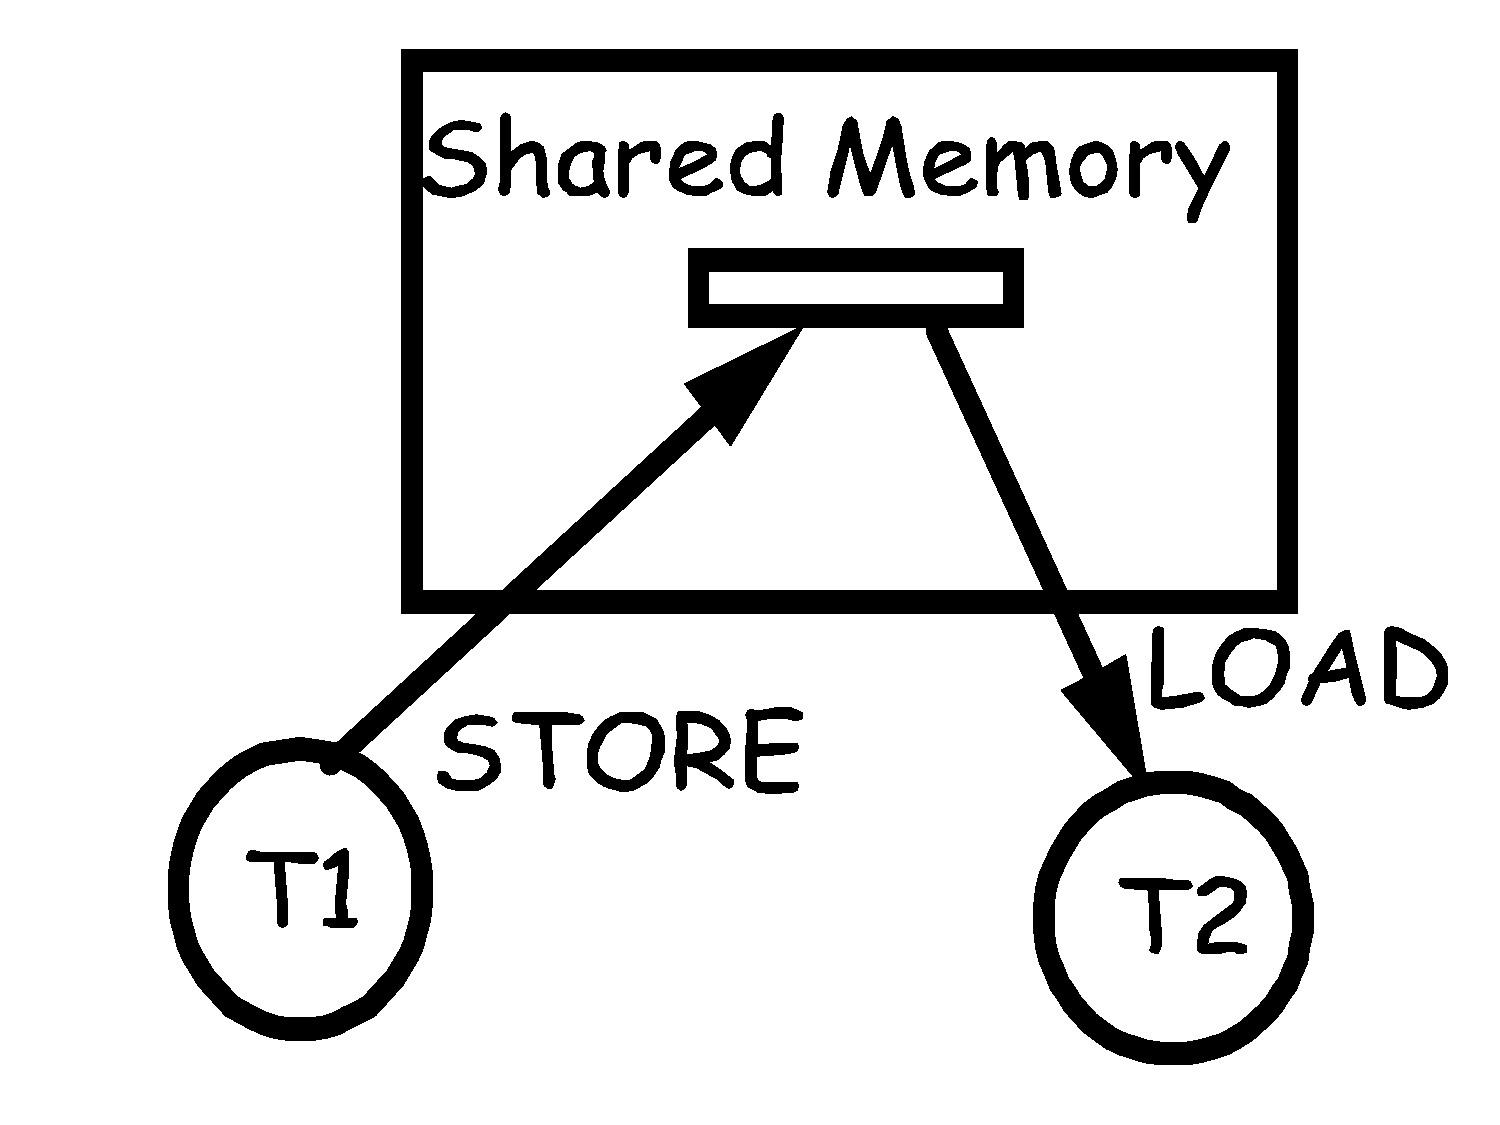
\includegraphics[width=27ex]{Ch7Figs/ShMem}\pause
\column{0.70\textwidth}
%\begin{scriptsize}
\begin{itemize}
    \item processors share memory \&\medskip
    \item communication implicit via loads and stores
    \begin{itemize}
        \item need to synchronize and\smallskip
        \item need to know how hwd may interleave 
                accesses from different processors.\medskip
        \item \alert{no assumption on the relative speed of processors}.
    \end{itemize}
\end{itemize}
%\end{scriptsize}
\end{columns}
\bigskip

In most cases, \emp{expect the multi-threaded program to behave identically with
sequential execution}, regardless of how many runs and processors are used. 

\end{frame}

%%%%%%%%%%%%%%%%%%%%%%%%%%%%%%%%%%%%%%%%%%%%%
%%%%%%%%%%%%%%%%%%%%%%%%%%%%%%%%%%%%%%%%%%%%%
%%%%%%%%%%%%%%%%%%%%%%%%%%%%%%%%%%%%%%%%%%%%%
\section{Synchronization Instructions}

\begin{frame}[fragile,t]
\frametitle{Synchronization}

\begin{block}{{\tt~~~~}Hight-Level Code:{\tt~~~~~~~~~~~~~~}Machine Code:{\tt~~~~~~~~~}}
\begin{columns}
\column{0.18\textwidth}
\begin{colorcode}[fontsize=\scriptsize]
\mymath{T\myindx{1}}
A \mymath{\leftarrow} A + 1





// \emph{User expects A incremented with 2}
\end{colorcode} 
\column{0.18\textwidth}
\begin{colorcode}[fontsize=\scriptsize]
\mymath{T\myindx{2}}
A \mymath{\leftarrow} A + 1






\end{colorcode}
\column{0.18\textwidth}\pause
\begin{colorcode}[fontsize=\scriptsize]
\mymath{T\myindx{1}}
r1 \mymath{\leftarrow} A

r1 \mymath{\leftarrow} r1 + 1

A \mymath{\leftarrow} r1

\alert{but result is A incremented by 1}
\end{colorcode} 
\column{0.18\textwidth}
\begin{colorcode}[fontsize=\scriptsize]
\mymath{T\myindx{2}}

r1 \mymath{\leftarrow} A

r1 \mymath{\leftarrow} r1 + 1

A \mymath{\leftarrow} r1

\end{colorcode} 
\end{columns}
\end{block}
\bigskip

%\emp{Need for Mutual Exclusion}, e.g., lock/unlock where modifications 
%are released at the end of critical section:

\begin{block}{Need Mutual Exclusion; \alert{How is it Implemented?}}
\begin{columns}
\column{0.2\textwidth}
\begin{colorcode}[fontsize=\scriptsize]
\mymath{T\myindx{1}}
lock(La)
A \mymath{\leftarrow} A + 1
unlock(La)
\end{colorcode} 
\column{0.2\textwidth}
\begin{colorcode}[fontsize=\scriptsize]
\mymath{T\myindx{2}}
lock(La)
A \mymath{\leftarrow} A + 1
unlock(La)
\end{colorcode} 
\column{0.49\textwidth}
Atomic Execution via lock/unlock,
where modifications are released
at the end of the critical section.
\end{columns}
\end{block}
 
\end{frame}


\begin{frame}[fragile,t]
\frametitle{Locking, Barrier, Point-to-Point Synchronization}

\begin{block}{Dekker's Lock/Unlock for the Simple, Two-Thread Case}
\begin{columns}
\column{0.24\textwidth}
\begin{colorcode}[fontsize=\scriptsize]
\mymath{T\myindx{1}}
\emph{A := 1}
while( \emp{B == 1} ) ;
<critical section>
\emph{A := 0}
\end{colorcode} 
\column{0.24\textwidth}
\begin{colorcode}[fontsize=\scriptsize]
\mymath{T\myindx{2}}
\emp{B := 1}
while( \emph{A == 1} ) ;
<critical section>
\emp{B := 0}
\end{colorcode} 
\column{0.4\textwidth}
\emp{Complex to solve deadlock and synch $>$ 2 threads.}\\
\emph{Use hardware primitives for the general case.}
\end{columns}
\end{block}

\begin{block}{Barrier and {\tt~~~~~~~~~~~~~~~~~~} Point-to-Point Synchronization}
\begin{columns}
\column{0.21\textwidth}
\begin{colorcode}[fontsize=\scriptsize]
\mymath{T\myindx{1}}
...
BAR := BAR + 1
while( BAR < 2 ) ;
...
\end{colorcode} 
\column{0.21\textwidth}
\begin{colorcode}[fontsize=\scriptsize]
\mymath{T\myindx{1}}
...
BAR := BAR + 1
while( BAR < 2 ) ;
...
\end{colorcode} 
\column{0.25\textwidth}
\begin{colorcode}[fontsize=\scriptsize]
\mymath{T\myindx{1}}


while( FLAG == 0 ) ;
print A
\end{colorcode} 
\column{0.18\textwidth}
\begin{colorcode}[fontsize=\scriptsize]
\mymath{T\myindx{2}}
A    := 1;
FLAG := 1;


\end{colorcode} 
\end{columns}
\end{block}
\medskip
\pause
 
\emp{Barrier}: all threads have to reach it before executing beyond it.
\begin{itemize}
    \item \alert{need critical section to increment {\tt BAR}} + \emph{read/reset {\tt BAR} fine}.
\end  {itemize}
\medskip

\emp{Point-to-Point}: no need for critical section; producer-consumer sync.

\end{frame}


\begin{frame}[fragile,t]
\frametitle{Jacobi Example}

\begin{columns}
\column{0.8\textwidth}
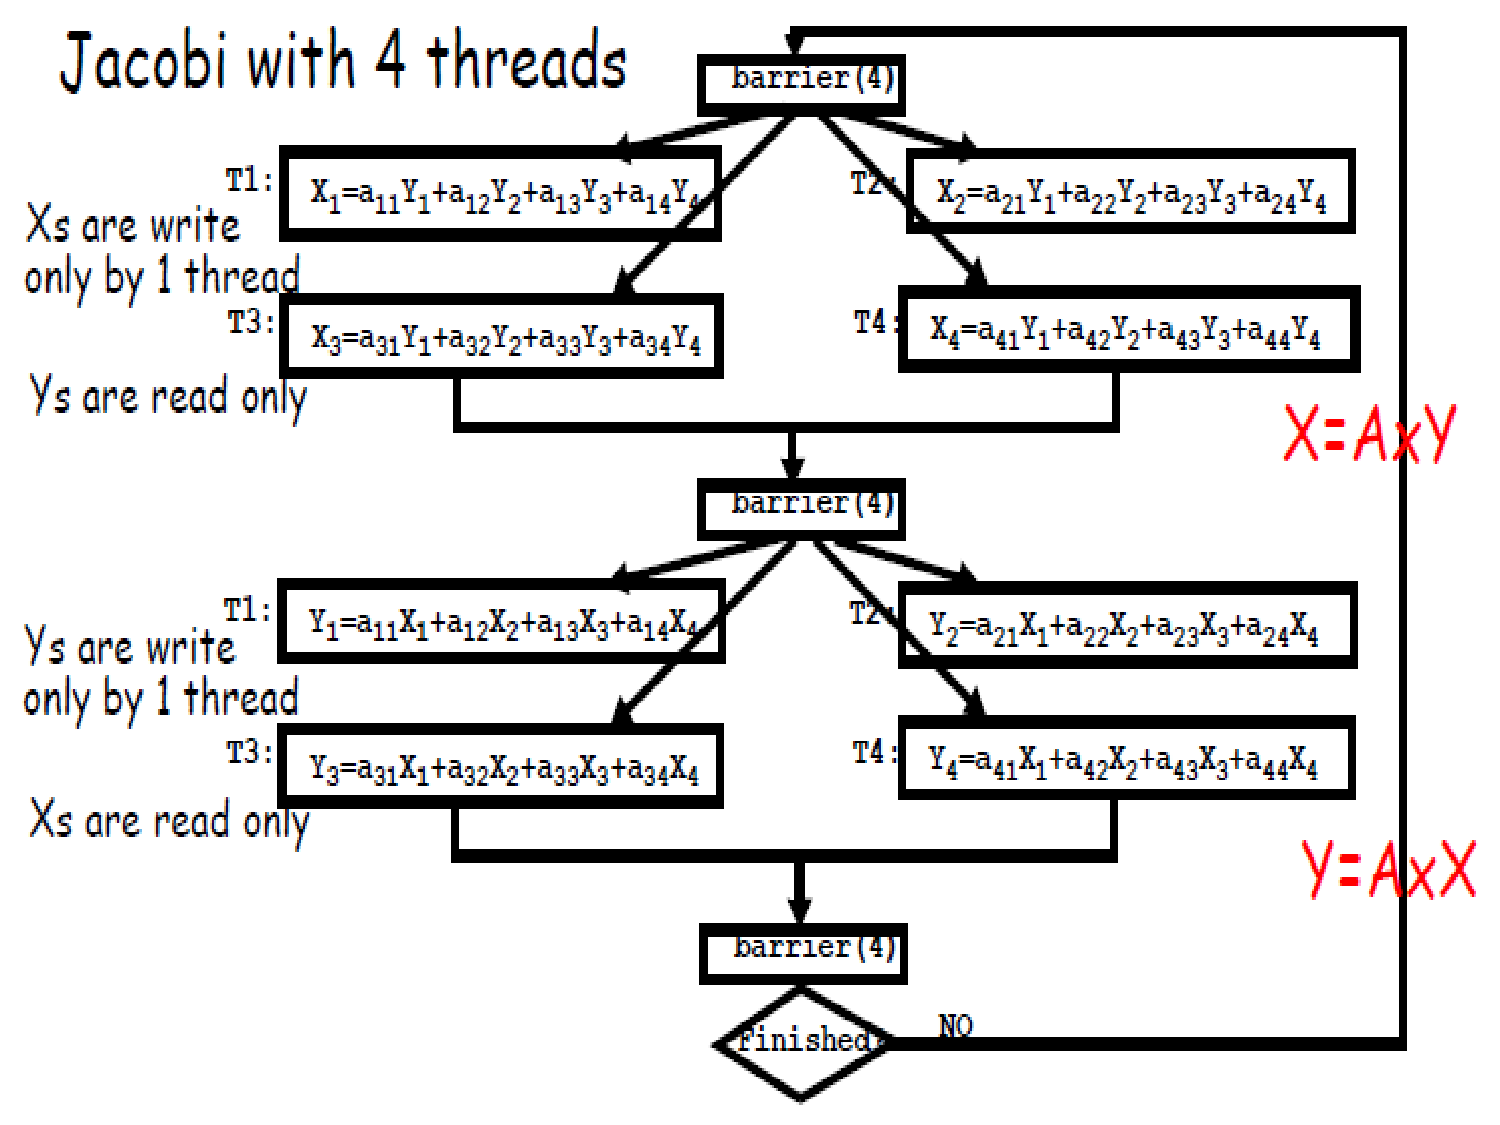
\includegraphics[width=58ex]{Ch7Figs/Jacobi}\pause
\column{0.3\textwidth}
%\begin{scriptsize}
\begin{itemize}
    \item Barriers separates the writes into {\tt X}s 
    \item from the read from {\tt X}s. 
    \item Same for {\tt Y}s.
\end{itemize}
%\end{scriptsize}
\end{columns}
\bigskip

\end{frame}


\begin{frame}[fragile,t]
\frametitle{Synchronization}

%\begin{scriptsize}
\begin{itemize}
    \item \emp{Acquire Method} (how to acquire rights to enter critical section)\medskip
    \item \emp{Release Method} (how to allow other processors to acquire rights)\medskip
    \item \emp{Waiting Algorithm}\smallskip
        \begin{itemize}
            \item \emp{Blocking}: waiting processes are descheduled
                \begin{itemize}
                    \item \alert{high overhead,} \emph{but allows processor to work on smth else.}
                \end  {itemize}\smallskip
            \item \emp{Busy Waiting}: releasing processor sets a location 
                        and waiting processors repeatedly check whether it is set:
                \begin{itemize}
                    \item \emph{low overhead}, \alert{but holds processor \& high memory traffic}
                \end  {itemize}\smallskip
            \item \emp{Hardware Multi-Threading}: consider it a long latency event and switch to others.
        \end  {itemize}\medskip
    \item \emph{Busy Waiting better when:}
        \begin{itemize}
            \item scheduling overhead $>$ expected wait time
            \item no other task to run or task is OpSys kernel.
        \end  {itemize}
\end{itemize}
%\end{scriptsize}

\end{frame}


\begin{frame}[fragile,t]
\frametitle{Locks}

%\begin{scriptsize}
\begin{itemize}
    \item \emp{Hardware Locks} (how to acquire rights to enter critical section)\smallskip
        \begin{itemize}
            \item separate \emp{lock lines on the bus}: holder of the lock asserts the line,
                    or barrier via open-collect connection.
            \item \emp{lock registers}: set of hardware registers.
            \item \alert{Poor scalability} shared resource other than memory \& its bandwidth limits the \# of processors connected to it, 
            \item \alert{Limited flexibility}, e.g., hardwired waiting alg, 
                    if more sync resources are needed then sync virtualized by software. 
            \item \alert{Complexity} hwd thread rather than core support needed.  
        \end  {itemize}\bigskip

    \item \emph{ISA Support: {\em most modern machine use a form of atomic read-modify-write (on Shared Memory)}}\smallskip
        \begin{itemize}
            \item IBM 370: atomic compare-and-swap (CAS),
            \item X86: any instruction can be prefixed with a lock,
            \item MIPS, PowerPC: support from pairs of instructions, 
                    e.g., load-locked (LL), store-conditional (SC) \& hwd ensure atomic exec of the two.
        \end  {itemize}\medskip
\end{itemize}
%\end{scriptsize}

\emph{These basic mechanisms are used to build software locks.}

\end{frame}


\begin{frame}[fragile,t]
\frametitle{Test And Set}

\begin{block}{Unsafe Software Lock{\tt~~~} Atomic Test And Set \& Optimized Traffic}
\begin{columns}
\column{0.33\textwidth}
\begin{colorcode}[fontsize=\scriptsize]
Lock:   
  \alert{LW   R2, lock}
  BNEZ R2, Lock //lock==0?
  \alert{SW   R1, lock} //lock:=1
  RET
Unlock: SW   R0, lock
        RET
\end{colorcode} 
\column{0.24\textwidth}\pause
\begin{colorcode}[fontsize=\scriptsize]
Lock:   \emp{T\&S R1, lock}
        BNEZ R1, Lock

        RET

Unlock: SW   R0, lock
        RET
\end{colorcode} 
\column{0.32\textwidth}\pause
\begin{colorcode}[fontsize=\scriptsize]
Lock:   \emph{LW   R1, lock}
        \emph{BNEZ R1, Lock}
        \emph{T\&S R1, lock}
        BNEZ R1, Lock
        RET
Unlock: SW   R0, lock
        RET
\end{colorcode}   
\end{columns}
\end{block}

\alert{Software lock}: read {\tt lock} (in {\tt R2}) until {\tt lock} is found to be {\tt 0}.
    Then set {\tt lock} to {\tt 1}. \alert{Problem: load and set of {\tt lock} not atomic.}\medskip

\emp{\tt T\&S R1, lock}: atomically reads {\tt lock} in {\tt R1} \& sets {\tt lock} to 1. 
\emp{Generates high memory traffic.}\medskip

\emph{Use cache protocol to reduce {\tt T\&S} frequency:} the first loop hits in cache.
Use {\tt T\&S} only when {\tt lock} is invalidated. Or with exponential backoff.

\end{frame}


\begin{frame}[fragile,t]
\frametitle{Other Read-Modify-Write Atomic Instructions}

\begin{itemize}
    \item \emp{\tt SWAP R1, MemLoc} exchanges the content of {\tt R1} and {\tt MemLoc}\bigskip

    \item Fetch\&Op, e.g., \emp{\tt F\&Add R1,MemLoc,c} fetches the value of {\tt MemLoc} in R1, 
            then increments {\tt MemLoc} by {\tt c},\bigskip

    \item Compare \& Swap, e.g., \emp{\tt CAS R1, R2, MemLoc} compares 
            value of {\tt MemLoc} with {\tt R1}, and if equal swaps {\tt R2} and {\tt MemLoc},\bigskip

    \item Load-Locked {\tt LL} and Store-Conditional {\tt SC}\smallskip
        \begin{itemize}
            \item \emp{\tt LL Rx, lock} reads {\tt lock} in {\tt Rx}\smallskip
            \item \emp{\tt SC Rn, lock} tries to updated value of {\tt lock} to {\tt Rn},\smallskip 
            \item {\tt SC} succeeds if no other thread wrote {\tt lock} since {\tt LL}\smallskip
            \item If {\tt SC} fails it does not write memory, but sets {\tt Rn} to zero.
        \end  {itemize}
\end  {itemize}

\end{frame}

\begin{frame}[fragile,t]
\frametitle{Load-Locked {\tt LL} and Store-Conditional {\tt SC}}

\emp{\tt LL \& SC} easier to implement in a pipeline and is a flexible mechanism:\\
fancier atomic ops implemented by adding code between {\tt LL} and {\tt SC}:
\begin{itemize}
    \item keep it simple so that {\tt SC} likely to succeed
    \item avoid irreversible instrs, e.g., causing exceptions, or stores.
\end  {itemize}

\begin{block}{Using LL and SC for T\&S {\tt~~~} CAS Implementations}\vspace{-2ex}
\begin{columns}
\column{0.41\textwidth}
\begin{colorcode}[fontsize=\scriptsize]
T\&S(Rx,lock):
    ADDI R1, R0, 1 //R1:=1
    LL   Rx, lock  //Rx:=lock
    SC   R1, lock  //sets lock (?)
    BEQZ R1, T\&S
    RET


\end{colorcode} 
\column{0.57\textwidth}
\begin{colorcode}[fontsize=\scriptsize]
CAS(Rx,Ry,X):
    ADD  R2, Ry, R0 //save Ry
    LL   R1, X
    BNE  Rx, R1, rr
    SC   R2, X      //attempt to store Ry
    BEQZ R2, CAS
    ADD  Ry, R1, R0 //return X in Ry
rr: RET
\end{colorcode} 
\end{columns}
\end{block}

{\tt SC} fails if detects intervening writes to {\tt lock} since {\tt LL}. Implem:
\begin{itemize}
    \item LL-bit set when LL executed, but bus interface snoops updates or 
            invalidate signals and resets LL-bit,
    \item SC tests LL-bit and fails if reset.
\end  {itemize}
\end{frame}

%%%%%%%%%%%%%%%%%%%%%%%%%%%%%%%%%%%%%%%%%%%%%%%%
%%%%%%%%%%%%%%%%%%%%%%%%%%%%%%%%%%%%%%%%%%%%%%%%
%%%%%%%%%%%%%%%%%%%%%%%%%%%%%%%%%%%%%%%%%%%%%%%%

\section{Memory Coherence}

\subsection{Problem Statement}

\begin{frame}[fragile]
	\tableofcontents[currentsection]
\end{frame}

\begin{frame}[fragile,t]
\frametitle{Memory Coherence: Problem Statement}

{\bf Refers to ordering of load/store instructions corresponding
to the same address.}

\begin{columns}
\column{0.7\textwidth}
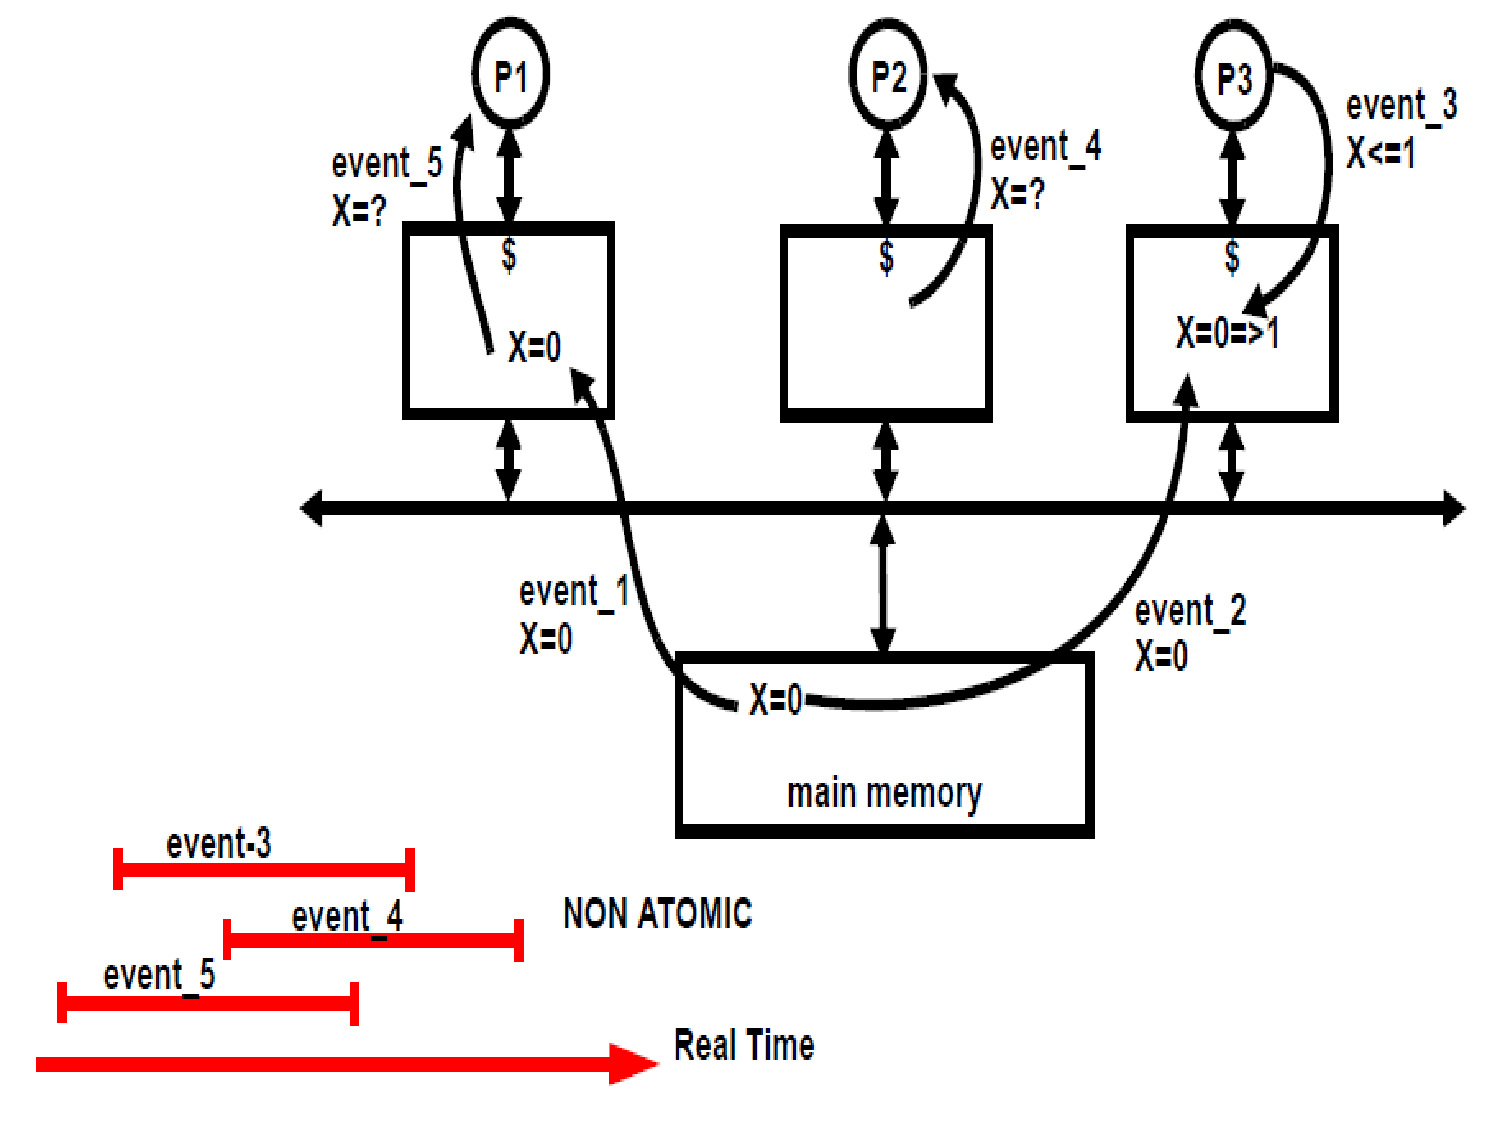
\includegraphics[width=50ex]{Ch7Figs/ProblemMemCoh}\pause
\column{0.38\textwidth}
%\begin{scriptsize}
\begin{itemize}
    \item {\tt event\_1/2/4/5}: Load {\tt X}
    \item {\tt event\_3}: Store 1 in {\tt X}
    \item Even assuming events do not overlap in time (atomic):
    \item Processors P1 and P3 ``see'' different values of X after {\tt event\_3}.  
\end{itemize}
%\end{scriptsize}
\end{columns}

\emph{Sufficient-Condition Solution: update or invalidate copies on updates. }

\end{frame}

\begin{frame}[fragile,t]
\frametitle{Why Is Coherence So Hard?}

\begin{itemize}
    \item After {\tt event\_3} caches contain different copies. Is this coherent?\smallskip
        \begin{itemize}
            \item YES, as long as P1 or P2 do {\bf not} execute their loads.
            \item a system remains coherent as long as incoherencies not detected.
        \end  {itemize}\bigskip

    \item Can the loads in events 4 and 5 return 0 or 1? Coherent?\smallskip
        \begin{itemize}
            \item both cases coherent because softw cannot detect the difference:
            \item P1 and P2 could have run slightly faster, so that they occur before event 3 in time.
        \end  {itemize}\medskip

    \item More Complex in practice because events are not atomic and sometimes overlap in time.\smallskip
        \begin{itemize}
            \item e.g., events 3,4,5 may be triggered in same clock
            \item they may proceed in parallel (time overlap)
                    on their hwd paths
            \item and if they conflict in some parts of hwd, they are serialized,
        \end  {itemize}\medskip

    \item Lets Assume first atomic coherence transitions (no time overlap):\smallskip
        \begin{itemize}
            \item helps understand how to propagate values effectively,
            \item protocol description at the behavioral level (no implem details)
        \end  {itemize}\medskip
\end{itemize}

\end{frame}


\subsection{Strict Coherence}

\begin{frame}[fragile,t]
\frametitle{Strict Coherence (SC)}

\begin{itemize}
    \item \emph{``Memory is coherent if the value returned by a Load
            is always the value of the latest store to the same 
            address.''}\medskip

    \item Fine for Uniprocessor, \emp{Difficult to extend to Multiprocessors}:
        \begin{itemize}
            \item execution time are unpredictable,
            \item inter-processor communication is NOT instantaneous.
        \end  {itemize}\smallskip

    \item \emp{Can be applied if}:
        \begin{itemize}
            \item memory accesses do not overlap in time, or
            \item \emp{stores are atomic}: all copies updated instantaneously, or
            \item store/load orders are enforced via synchronization 
                    primitives, i.e., by accesses to other memory locations.
        \end  {itemize}\smallskip

    \item \emp{Notations:}
\end{itemize}
\vspace{-3ex}

\center{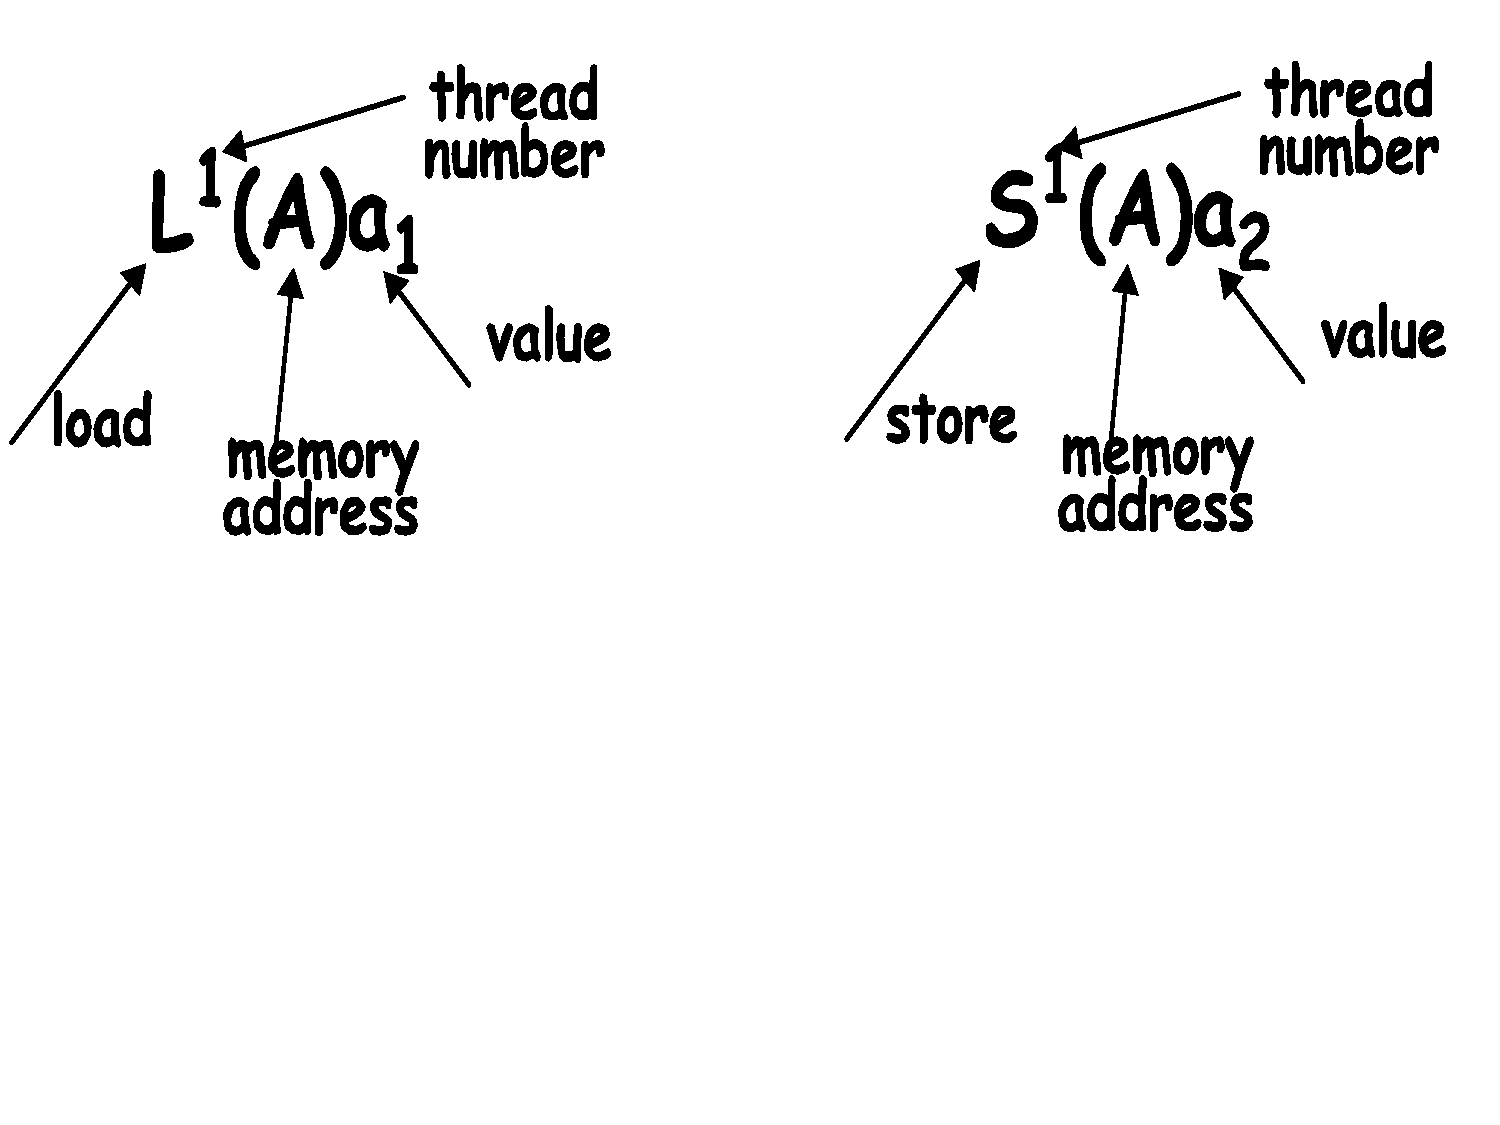
\includegraphics[width=44ex]{Ch7Figs/Notation1}}

\end{frame}

\subsection{Store Atomicity}

\begin{frame}[fragile,t]
\frametitle{Store Atomicity}

\begin{itemize}
    \item Coherence Transactions do not happen instantaneously
    \begin{itemize}
        \item enough to make them look atomic to the software,e.g.,databases.
    \end{itemize}\medskip

    \item \emp{\bf Condition: at any time, all threads must observe the same value for a memory location.} 
                \emp{Definition:} 
                %only one value of a memory location is accessible at any time.} \emp{Def:}
    \begin{itemize}
        \item[1] \emp{A load is performed} at the point in time when 
                    its value is bound and cannot be recalled, e.g., when value is used.
        \item[2] \emp{A store is performed w.r.t. thread $i$} when a load 
                    to thread $i$ cannot return a value prior to the store.
        \item[3] \emp{A store is globally performed} when is performed 
                    w.r.t. all threads,
        \item[4] \emp{A load is globally performed (GP)} when it is performed and 
                    the store providing the value is also globally performed. 
    \end{itemize}\medskip
%{\tiny (NOT NECESSARY)}
    \item \emph{{\bf Sufficient Condition for Store Atomicity}:}\pause
    \begin{itemize}
        \item[1] For any address, a global order of stores to that address exists \alert{and}
        \item[2] A load must be globally performed before its value can be used!\medskip
        \begin{itemize}
            \item Load value being bound and its store being globally performed 
            \item means that no thread can observe a new value while another thread
                    can still observe the old value.
        \end{itemize}

    \end{itemize}
\end{itemize}

\end{frame}


\begin{frame}[fragile,t]
\frametitle{Recall Write-Back MSI Invalidate Protocol}

\begin{itemize}
    \item \emp{Block States}: 
        \begin{itemize}
            \item Invalid (I): not in cache or coherence invalidation,
            \item Shared (S): one copy or more, memory is clean,
            \item Dirty or Modified (M): one copy, memory is stale.
        \end  {itemize}\smallskip

    \item \emp{Processor Requests}: write ({\tt PrWr}) or read ({\tt PrRd}).\smallskip

    \item \emp{Bus Transactions}:
        \begin{itemize}
            \item {\tt BusRd}: request copy with no modify intent,
            \item {\tt BusRdX}: request copy with intent to modify,
            \item {\tt Flush}: forward copy to requester and update memory in parallel,
            \item Write to shared block could use {\tt BusUpgr} instead of {\tt BusRdX}
        \end  {itemize}
\end{itemize}
\vspace{-2ex}

\center{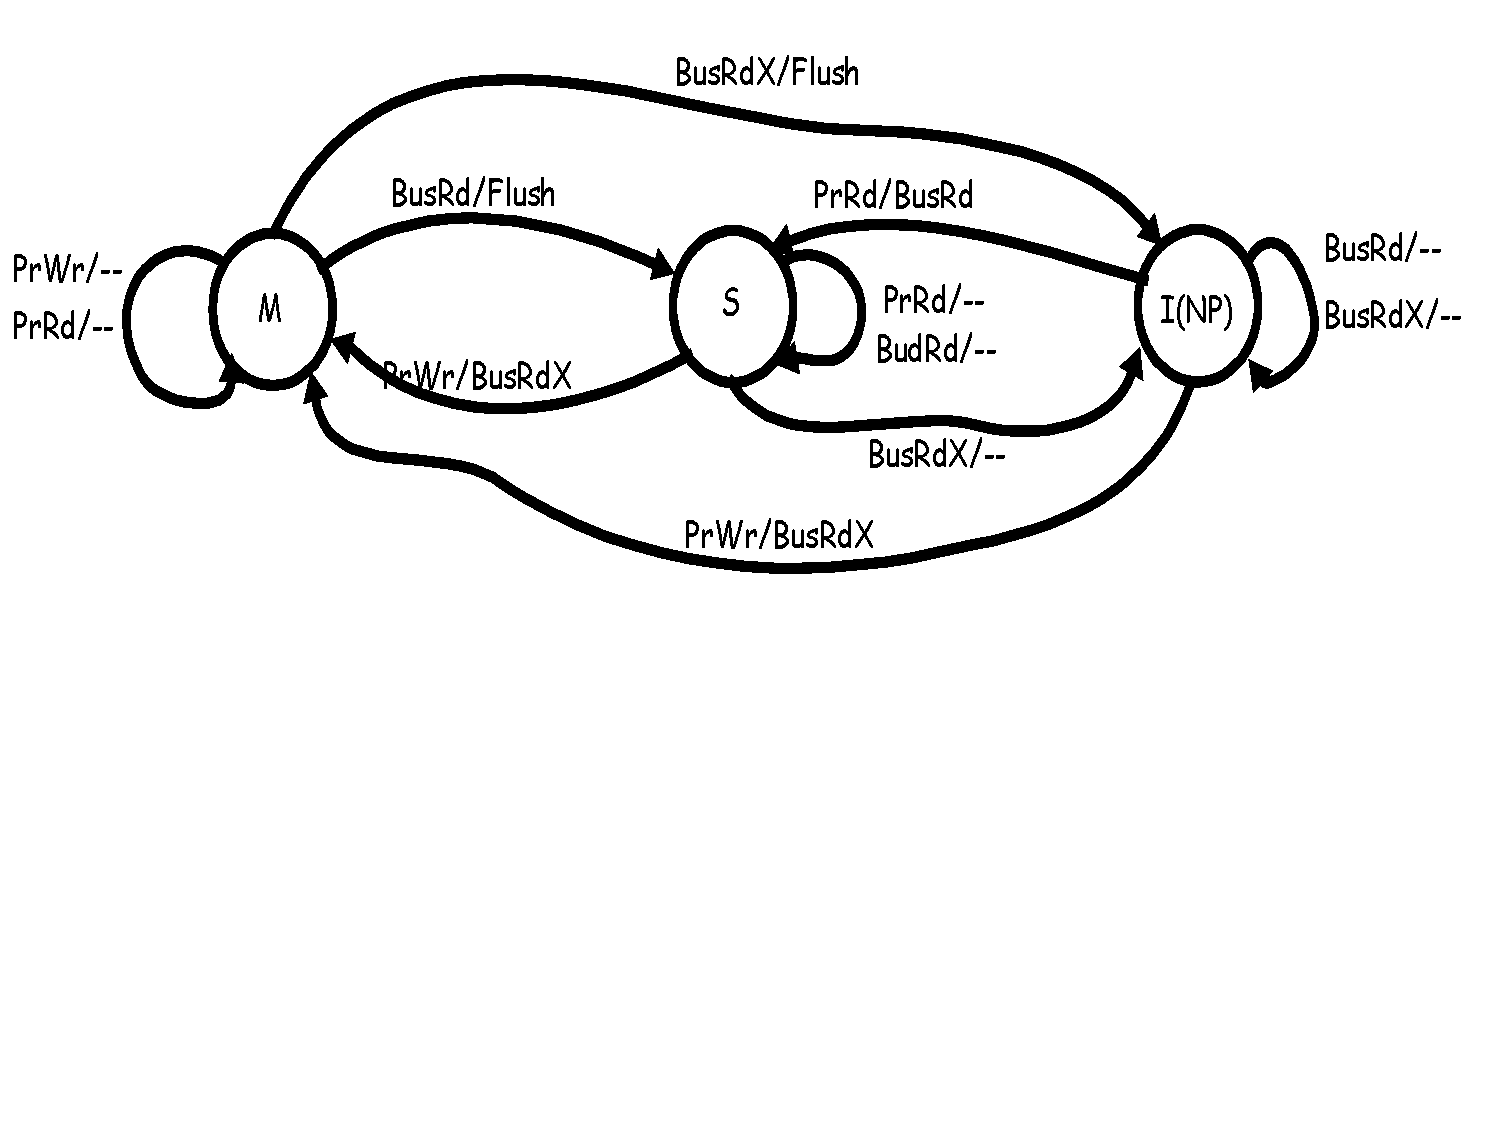
\includegraphics[width=55ex]{Ch7Figs/MSIinval}}

\end{frame}

\begin{frame}[fragile,t]
\frametitle{Recall Write-Back MSI Update Protocol}

\begin{itemize}
    \item \emp{Block States}: I, M as before, Shared: multiple copies, clean mem

    \item \emp{Processor Requests}: write ({\tt PrWr}) or read ({\tt PrRd}).\smallskip

    \item \emp{Bus Transactions}:
        \begin{itemize}
            \item {\tt BusRd}: request copy with no modify intent,
            \item {\tt BusUpdate}: update remote copies,
            \item {\tt Flush}: forward copy to requester and update memory in parallel,
            \item \emp{Shared Bus Line ({\tt S}) indicates whether remote copies exist.}
        \end  {itemize}
\end{itemize}
\vspace{-3ex}

\center{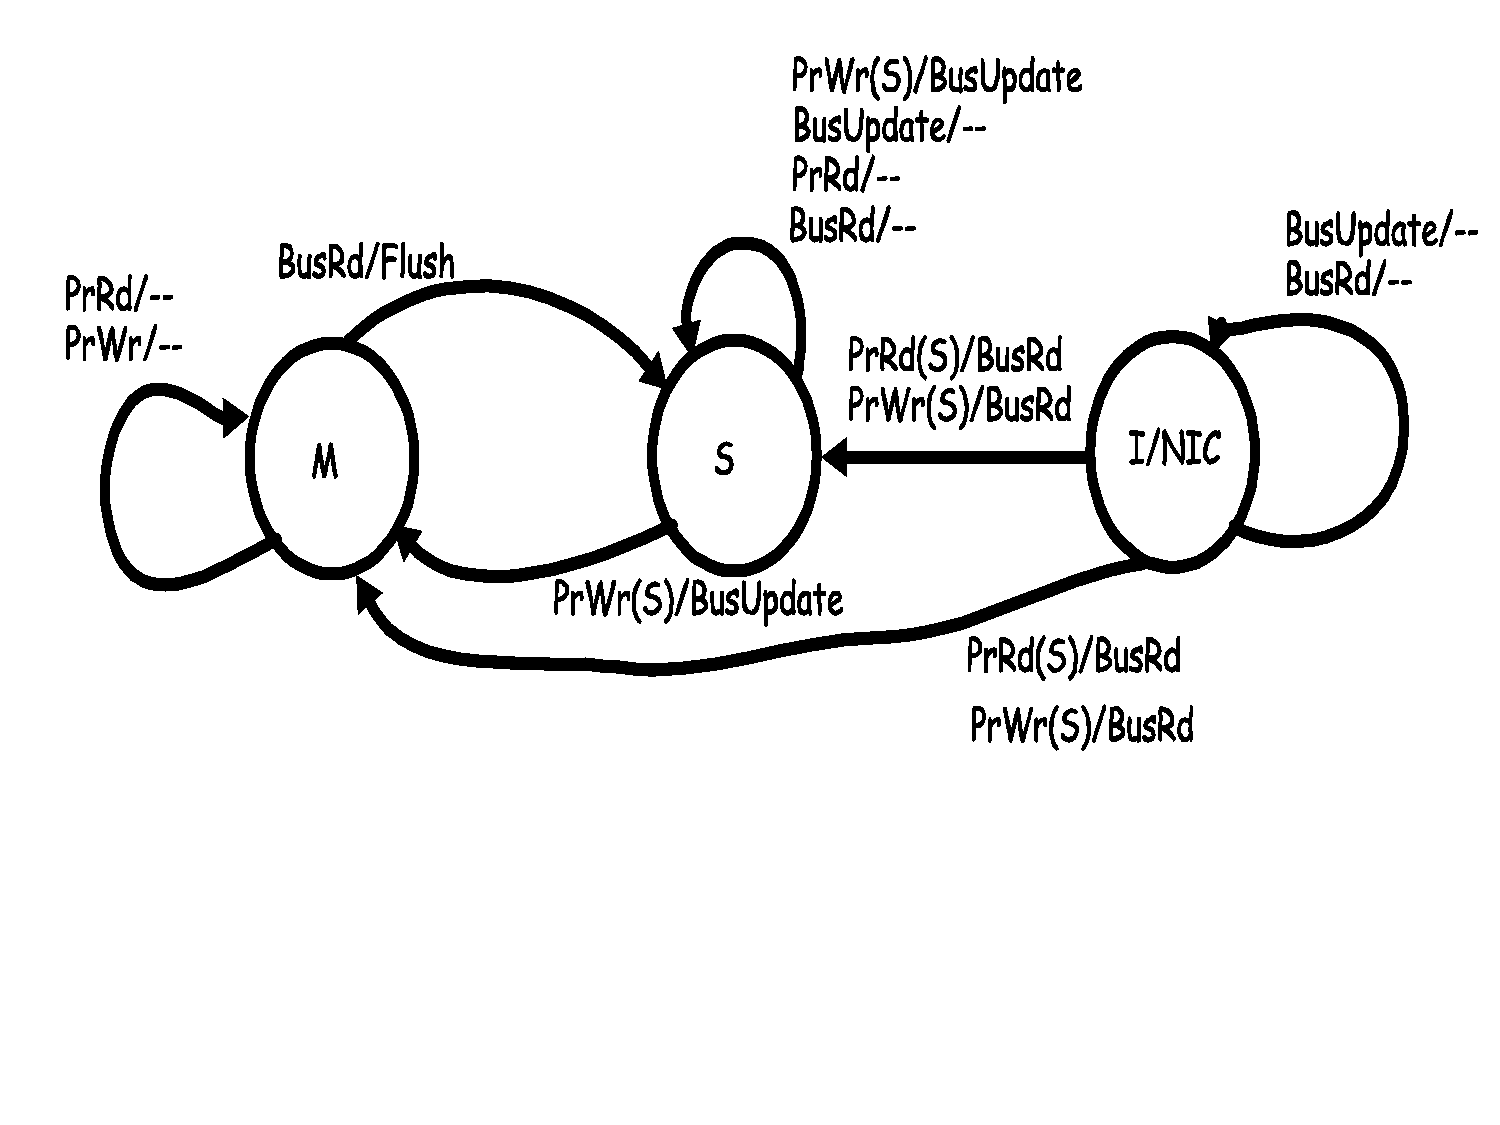
\includegraphics[width=55ex]{Ch7Figs/MSIupdate}}

\end{frame}


\begin{frame}[fragile,t]
\frametitle{Atomic Memory References}

Strict coherence can be applied if accesses to all memory locations are atomic,
i.e., do not overlap in time.  Store atomicity would allow $L^1(A)a_2$ and 
$L^2(A)a_2$ to overlap.

\begin{block}{Example using MSI invalidate{\tt~~~~~~~~~~} Comments}
\begin{columns}
\column{0.25\textwidth}
\begin{colorcode}[fontsize=\scriptsize]
CLK: T1:
t1:  S\mymath{\myindu{1}}(A)a\mymath{\myindx{1}}
t2:  L\mymath{\myindu{1}}(A)a\mymath{\myindx{1}}
t3:  S\mymath{\myindu{1}}(A)a\mymath{\myindx{2}}
t4:  L\mymath{\myindu{1}}(A)a\mymath{\myindx{2}}
t5:  ------------------
t6:  L\mymath{\myindu{1}}(A)a\mymath{\myindx{2}}
t7:  
t8:  L\mymath{\myindu{1}}(A)a\mymath{\myindx{2}}
t9   ------------------
t10: 
t11: S\mymath{\myindu{1}}(A)a\mymath{\myindx{4}}-----------
t13: S\mymath{\myindu{1}}(A)a\mymath{\myindx{5}}
\end{colorcode} 
\column{0.20\textwidth}
\begin{colorcode}[fontsize=\scriptsize]
T2:




L\mymath{\myindu{2}}(A)a\mymath{\myindx{2}}-----------

L\mymath{\myindu{2}}(A)a\mymath{\myindx{2}}

S\mymath{\myindu{2}}(A)a\mymath{\myindx{3}}-----------
L\mymath{\myindu{2}}(A)a\mymath{\myindx{3}}
------------------

\end{colorcode} 
\column{0.45\textwidth}\pause
\begin{scriptsize}
\emp{APT} = Atomic Protocol Transaction\\
\begin{itemize}
    \item Data not in C2\\
            and dirty in C1\\
            {\tt~~}\\
            {\tt~~}\\

    \item[\emp{APT1}:] Read Miss in C2;\\
                        A becomes shared in C1 and C2;\\
                        Both threads can read A, but\\
                        none may write A.
    \item[\emp{APT2}:] C1 is invalidated and\\ 
                      C2 becomes dirty
    \item[\emp{APT3:}] Store Miss in C1; C1 is dirty and\\
                        C2 is invalidated
\end{itemize}
\end{scriptsize}
\end{columns}
\end{block}

\end{frame}


\begin{frame}[fragile,t]
\frametitle{Store Atomicity in cc-NUMAs}

Assume cc-NUMA with MSI invalidate protocol, and a
write miss in {\tt T0} in the presence of two remote shared copies ({\tt T1} and {\tt T2}): 

\begin{columns}
\column{0.59\textwidth}
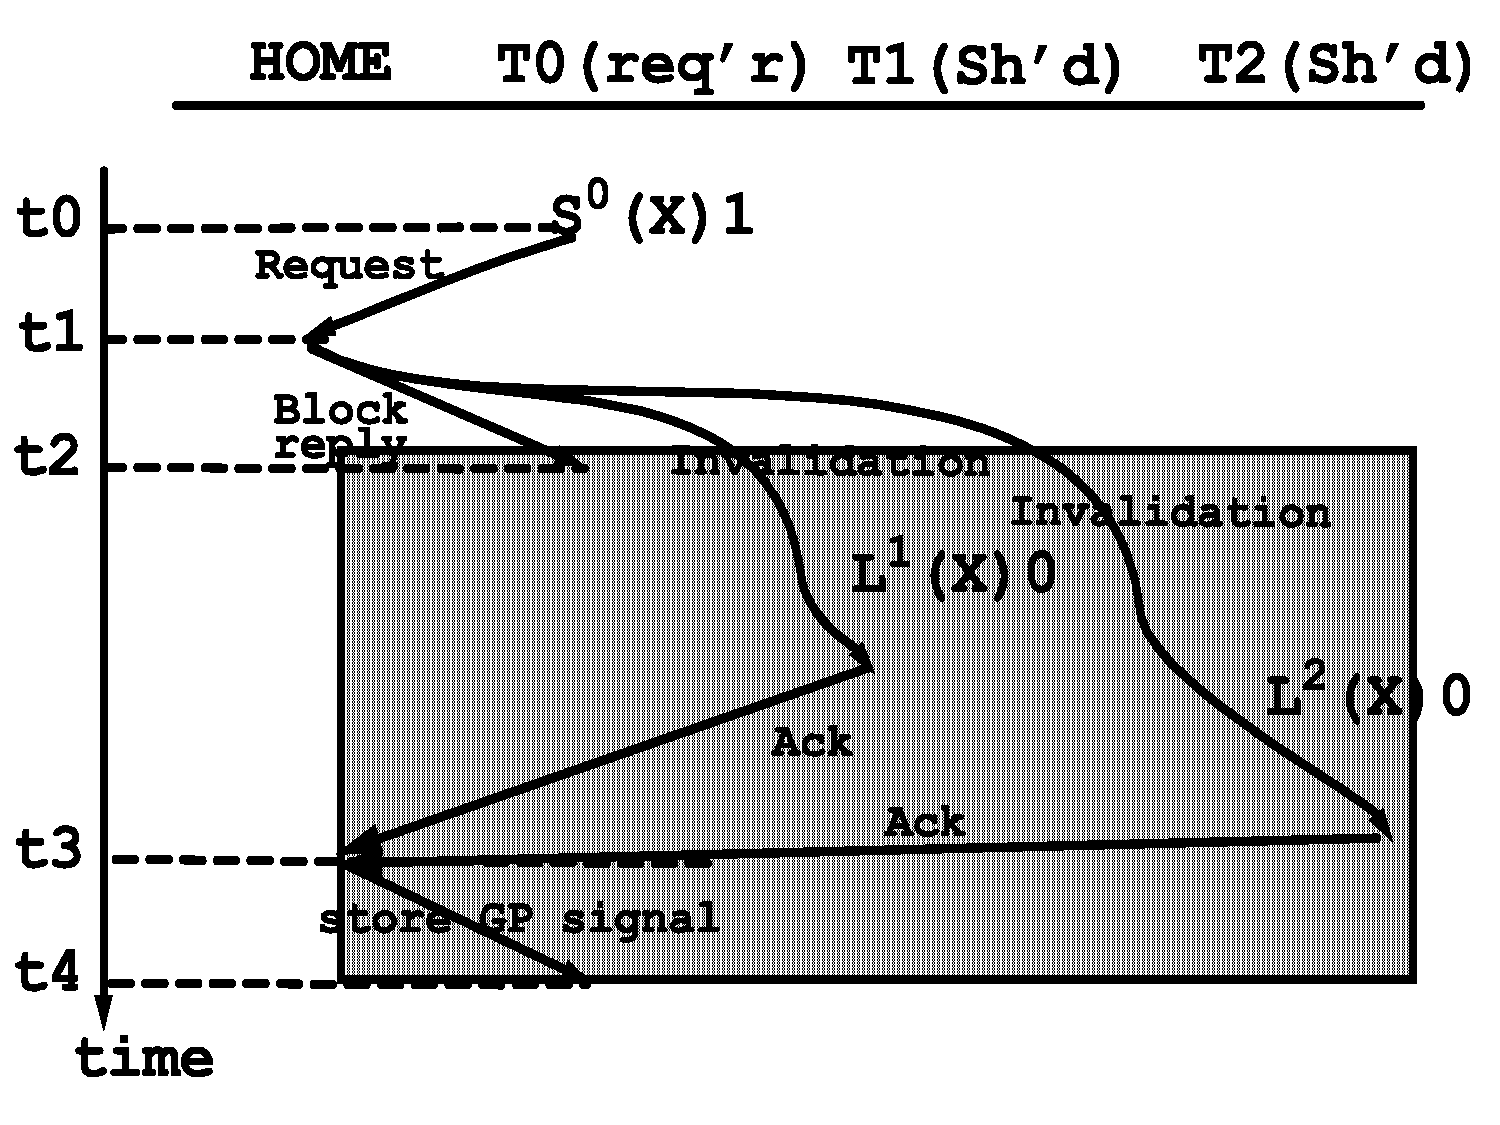
\includegraphics[width=44ex]{Ch7Figs/StoreAtomccNUMA}\pause
\column{0.39\textwidth}
\begin{scriptsize}
\begin{itemize}
    \item[t0:] {\tt BusRdX} sent to home (H)
    \item[t1:] H receives req and sets the busy bit
                (locking directory forces a global order).
                Finally, H sends a block copy to T0,
                and invalidations to T1 and T2.
    \item[t3:] H receives ACKs from T1 and T2, resets the busy bit
                and signals T0 that store access is globally performed.
    \item[t4:] receives ACK from H, completes store and proceeds. 
\end{itemize}
\end{scriptsize}
\end{columns}

\alert{Is the depicted behavior store atomic?}\\
\alert{What could have went wrong here?}

\end{frame}

\begin{frame}[fragile,t]
\frametitle{Store Atomicity in cc-NUMAs (Cont)}

\begin{columns}
\column{0.59\textwidth}
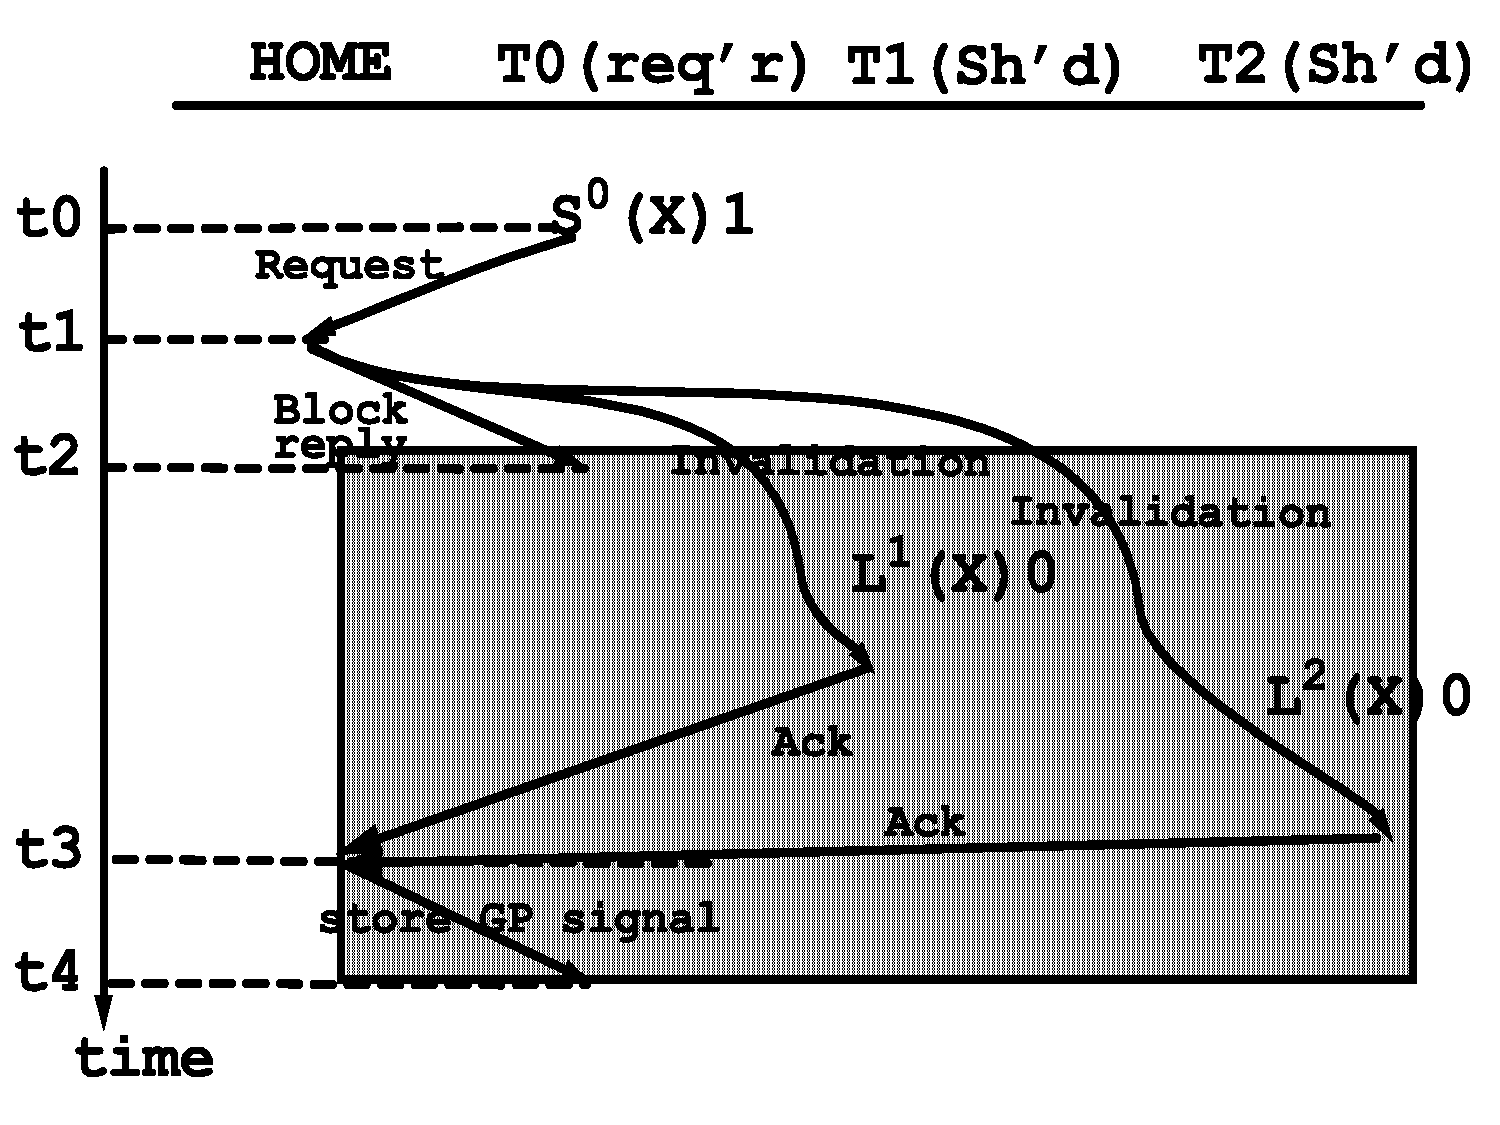
\includegraphics[width=44ex]{Ch7Figs/StoreAtomccNUMA}\pause
\column{0.30\textwidth}
Directory locks entry from {\tt t1} to {\tt t3}.
\alert{Should home send copy to T0 at t1 or t3?}
\end{columns}
\pause

\emph{For store atomicity:} Home can send copy to T0 either at {\tt t1} (better)
or {\tt t3}, but T0 must not return values from its stores (including the
one following the miss) until {\tt t4}, nor give them away.
That's because the store is globally performed at {\tt t3}!
\medskip

\emp{For plain coherence}, see next, the block can be released to T0 at {\tt t2}!

\end{frame}

\subsection{Plain Coherence}

\begin{frame}[fragile]
	\tableofcontents[currentsubsection]
\end{frame}

\begin{frame}[fragile,t]
\frametitle{Memory-Access Atomicity Relativity}

\begin{itemize}
    \item P2 has a Modified (unique) copy of {\tt X} in its cache
    \item when the load from P1 misses (in P1's cache)
\end{itemize}

{\center 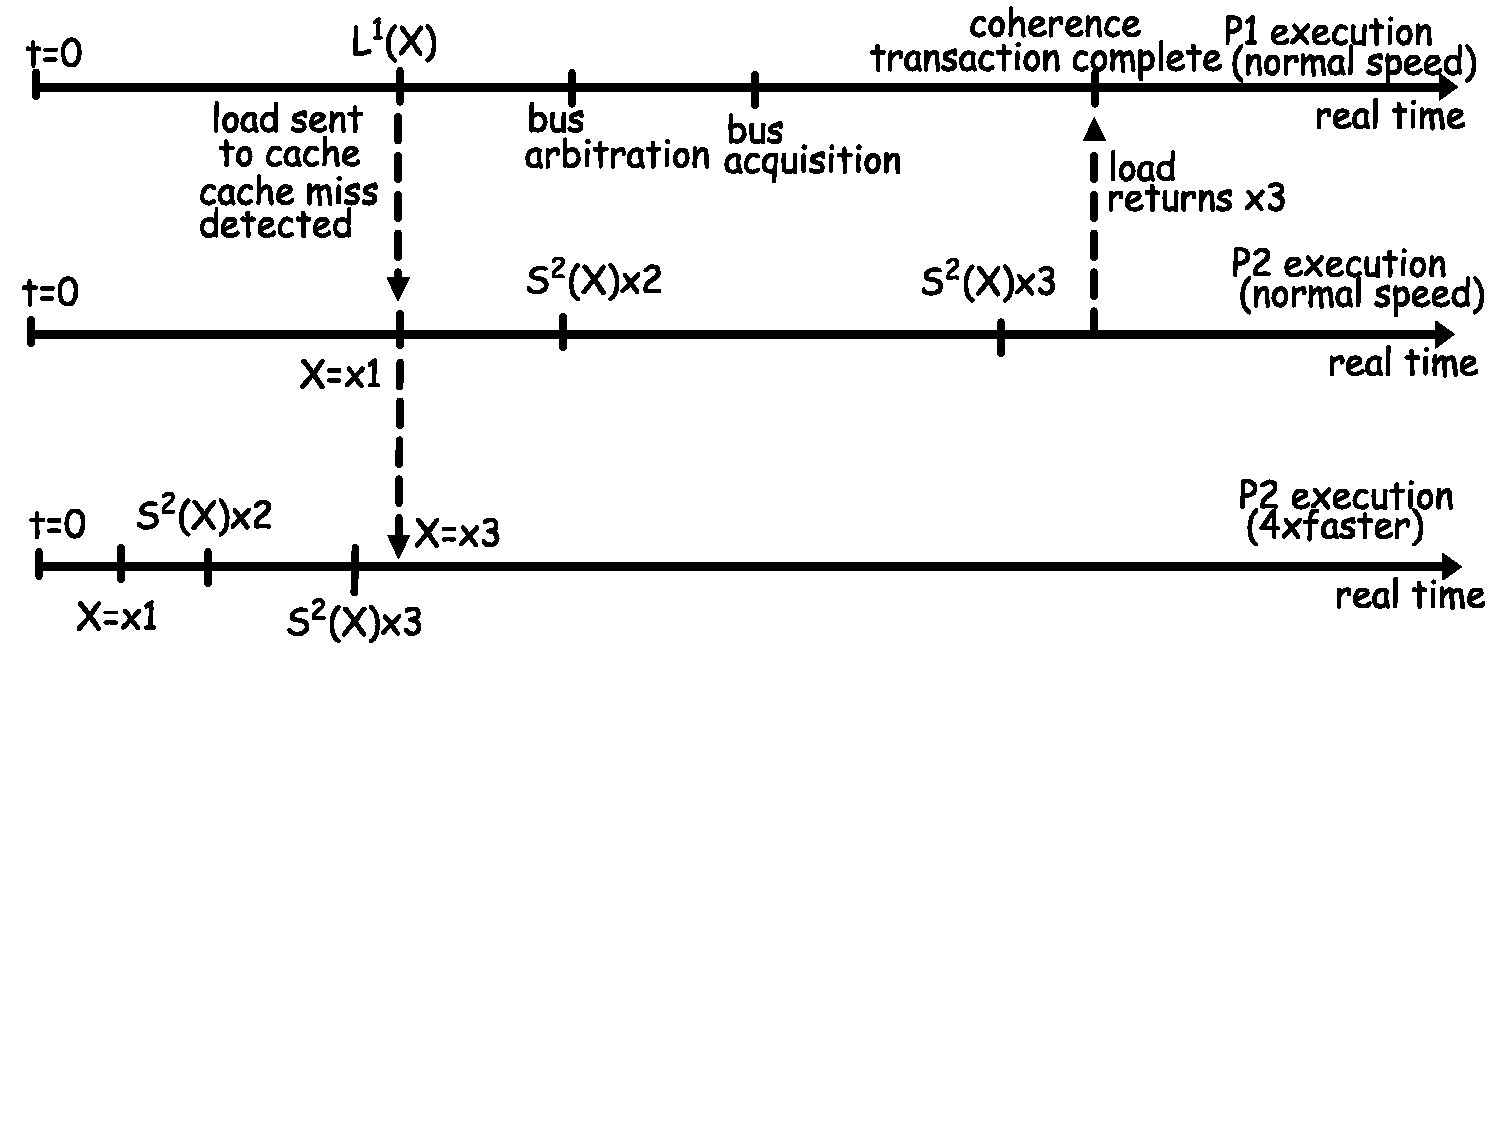
\includegraphics[width=59ex]{Ch7Figs/CoherenceEG1}}\pause
\vspace{-18ex}

\emp{Idea: enough to find an ordering of atomic instructions that ``makes sense''}, e.g.,
even with instantaneous loads, a program using shared memory 
cannot detect the difference between the load returning {\tt x1} or 
{\tt x3}, simply because if P2 would be 4$\times$ faster it would return {\tt x3}.

\end{frame}


\begin{frame}[fragile,t]
\frametitle{Today Coherence Transaction are Non-Atomic}

{\center 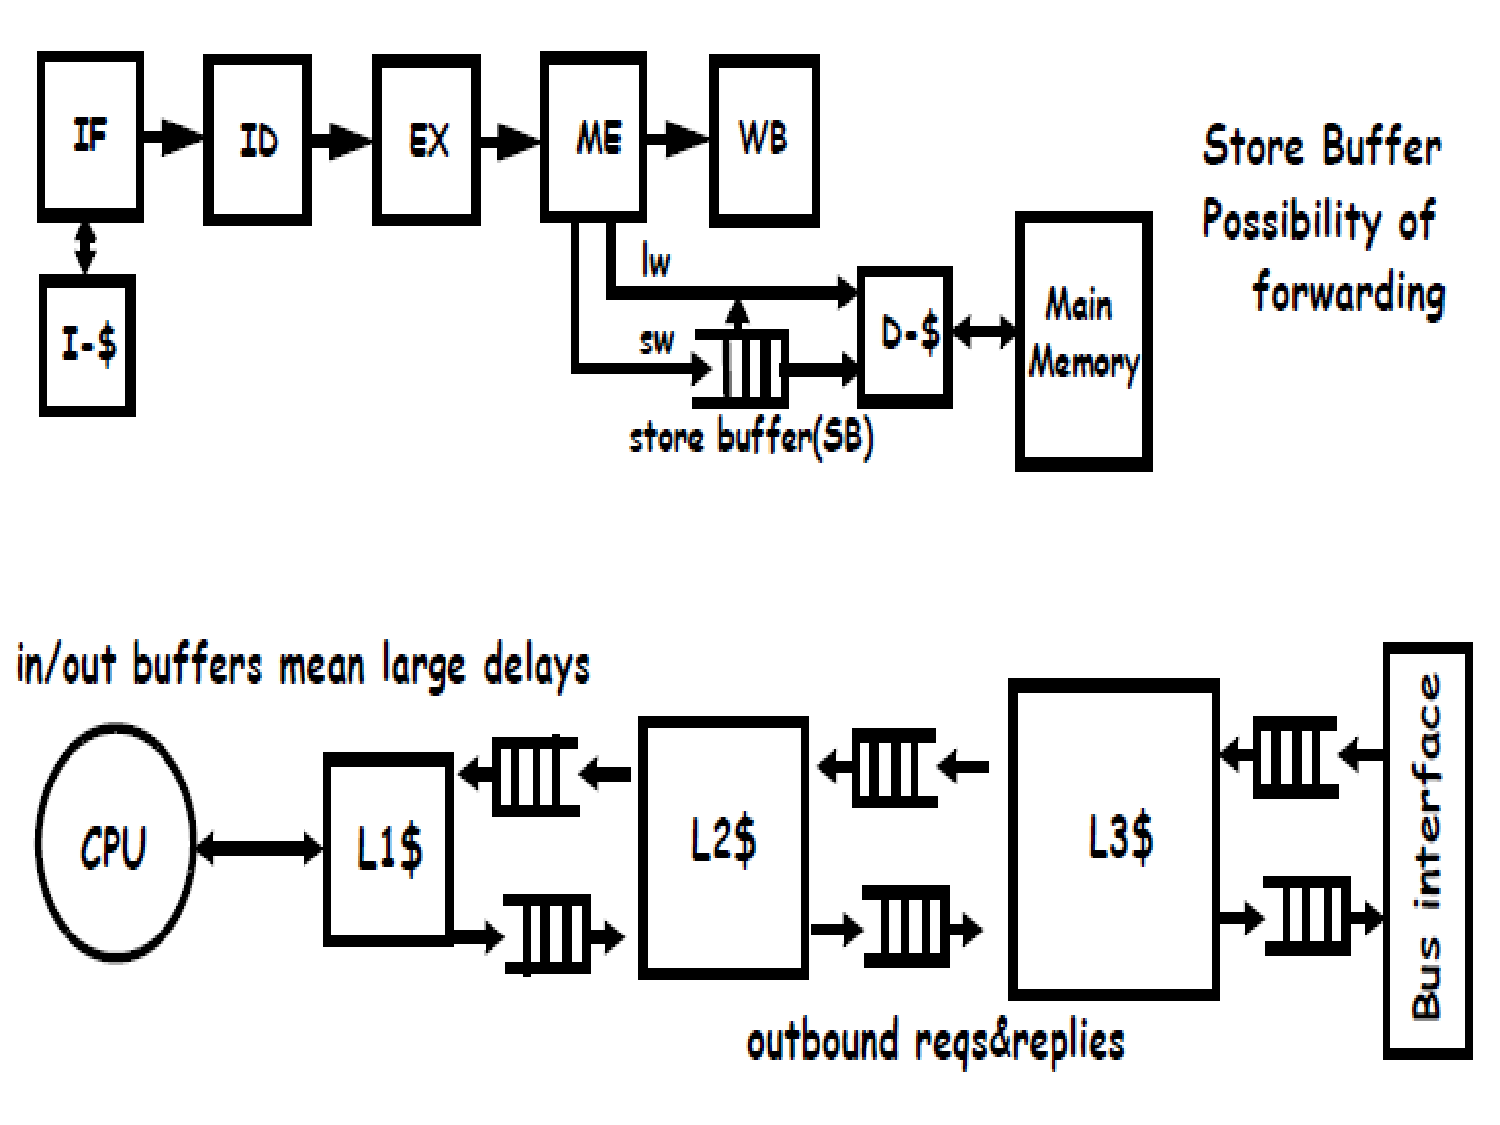
\includegraphics[width=59ex]{Ch7Figs/SoteBuffs}}

\end{frame}

\begin{frame}[fragile,t]
\frametitle{Today Coherence Transaction are Non-Atomic}

\begin{columns}
\column{0.3\textwidth}
\vspace{+7ex}
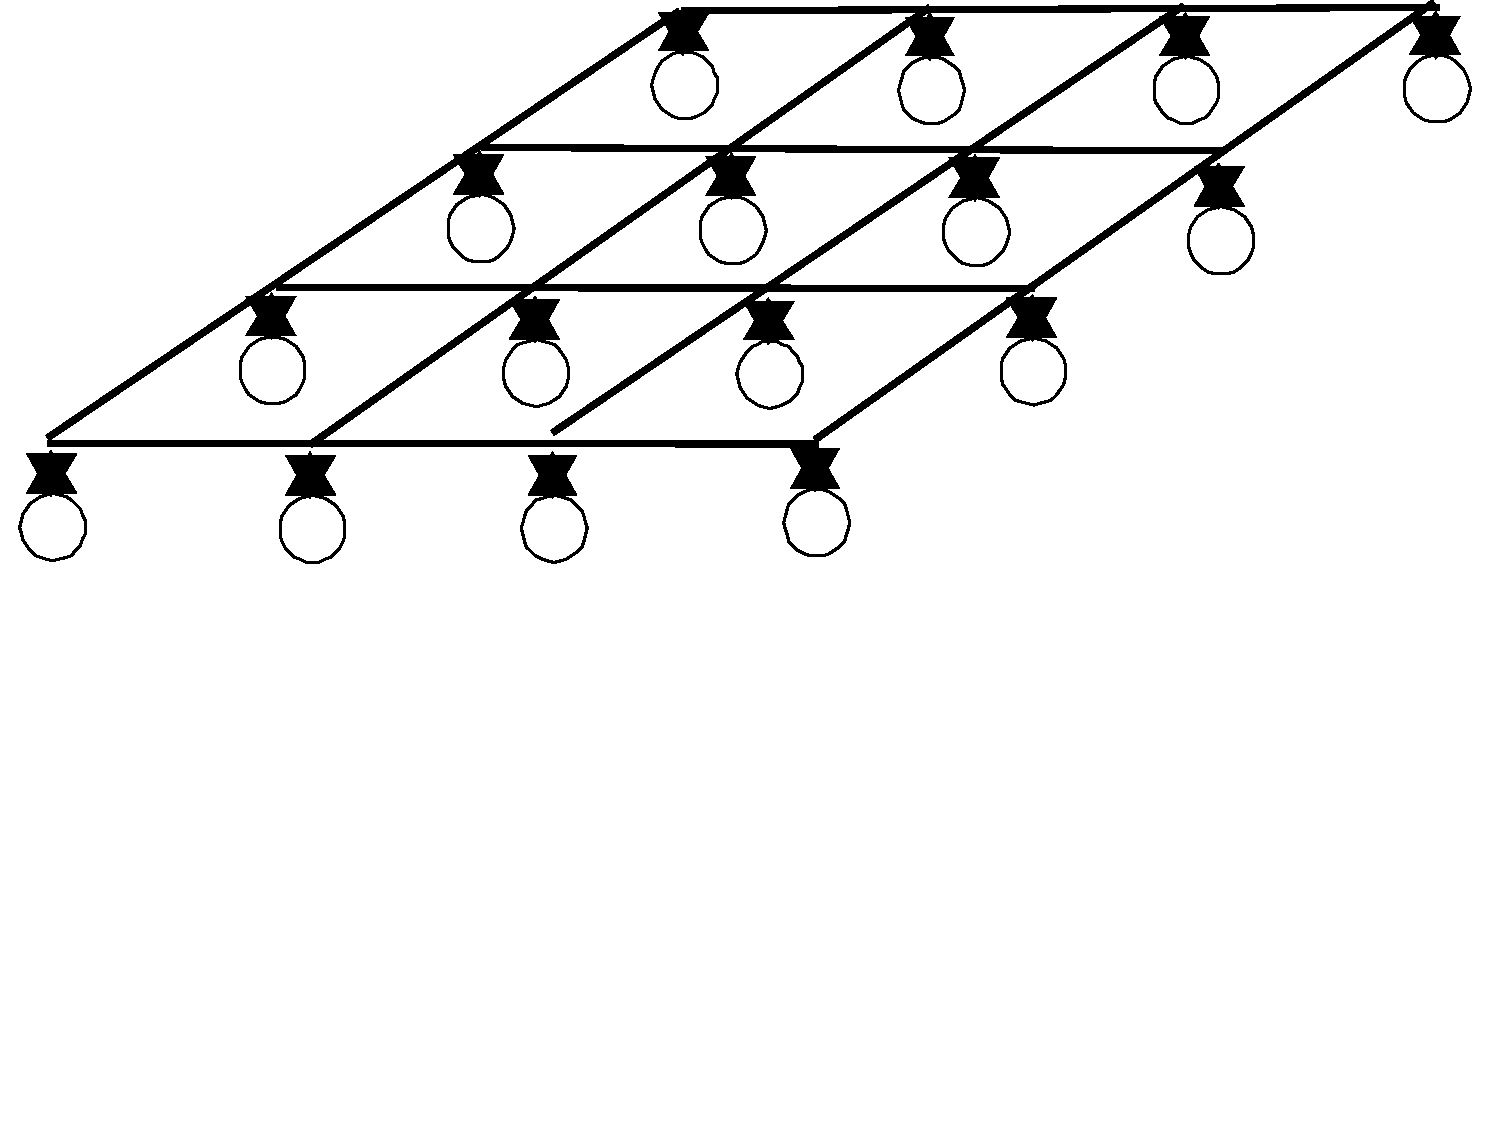
\includegraphics[width=22ex]{Ch7Figs/Mesh}\pause
\column{0.65\textwidth}
%\begin{scriptsize}
Packet or Circuit-switched interconnect
\begin{itemize}
    \item many routes between two points,
    \item adaptive routing to optimize congestion
    \item very unpredictable transmission times
\end{itemize}
\end{columns}

\end{frame}

\begin{frame}[fragile,t]
\frametitle{Plain Coherence: A Weaker Coherence}

\begin{itemize}
    \item Establish an order of all accesses to the same address,
    \item then apply the general definition of coherence, where \emp{latest}
    \begin{itemize}
        \item is not latest in the temporal sense,
        \item but rather in the established order of all accesses.
    \end  {itemize}\medskip

    \item {\bf Formal Model:}\\
            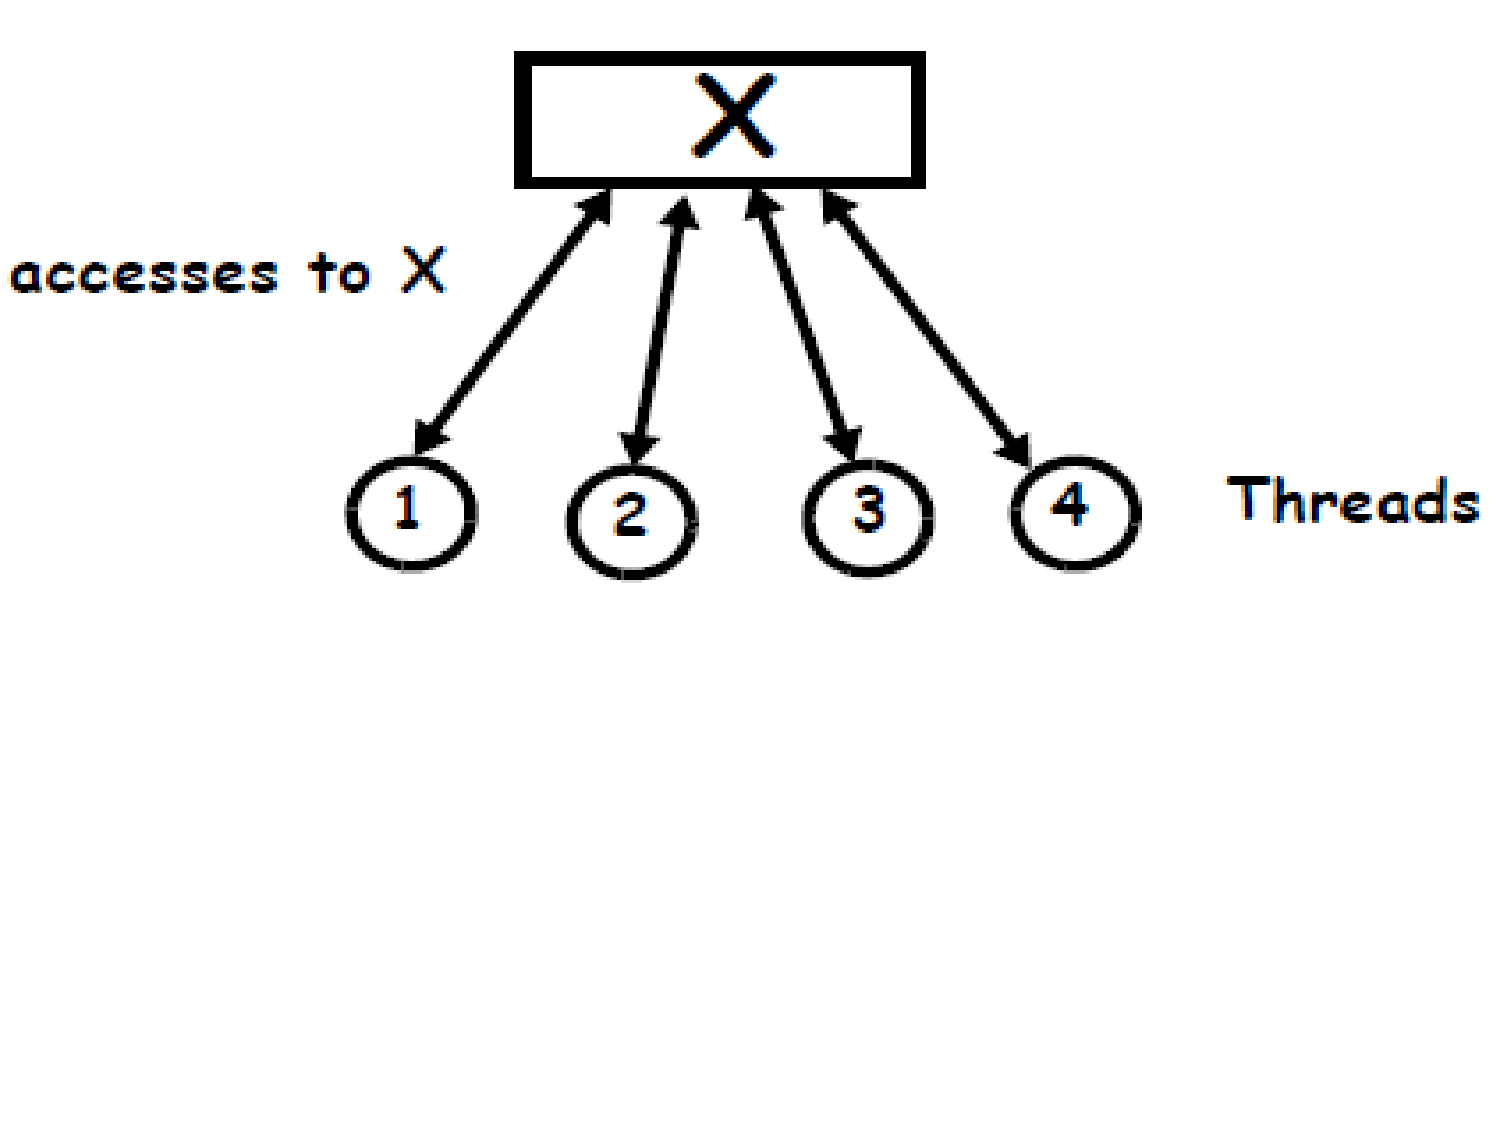
\includegraphics[width=33ex]{Ch7Figs/PlainCoh1}\vspace{-13ex}
    
    \item {\bf Rules of the Model:}
    \begin{itemize}
        \item each data/block has a single copy at any time,
        \item accesses respect the (intra) thread order.
    \end  {itemize}\medskip

    \item \emp{\bf System is Plain Coherent if its memory accesses to each address
            can be executed correctly in thread order in a system with one single copy
            of each memory address.}
\end{itemize}

\end{frame}


\begin{frame}[fragile,t]
\frametitle{Plain Coherence: Formal Definition}

\begin{itemize}
    \item {\bf ``System is Plain Coherent iff, for every execution and for any 
            memory location, it is possible to construct a total order of all memory operations
            to each location such that:}
    \begin{itemize}
        \item[1] {\bf mem ops of each thread to the location are in thread order,}
        \item[2] {\bf and the value returned by a load is the value of the latest store to the location
                in total (serial) order.}"
    \end  {itemize}\medskip


    \item Note: accesses by each thread must appear in thread order, but not necessarily in temporal order\\
            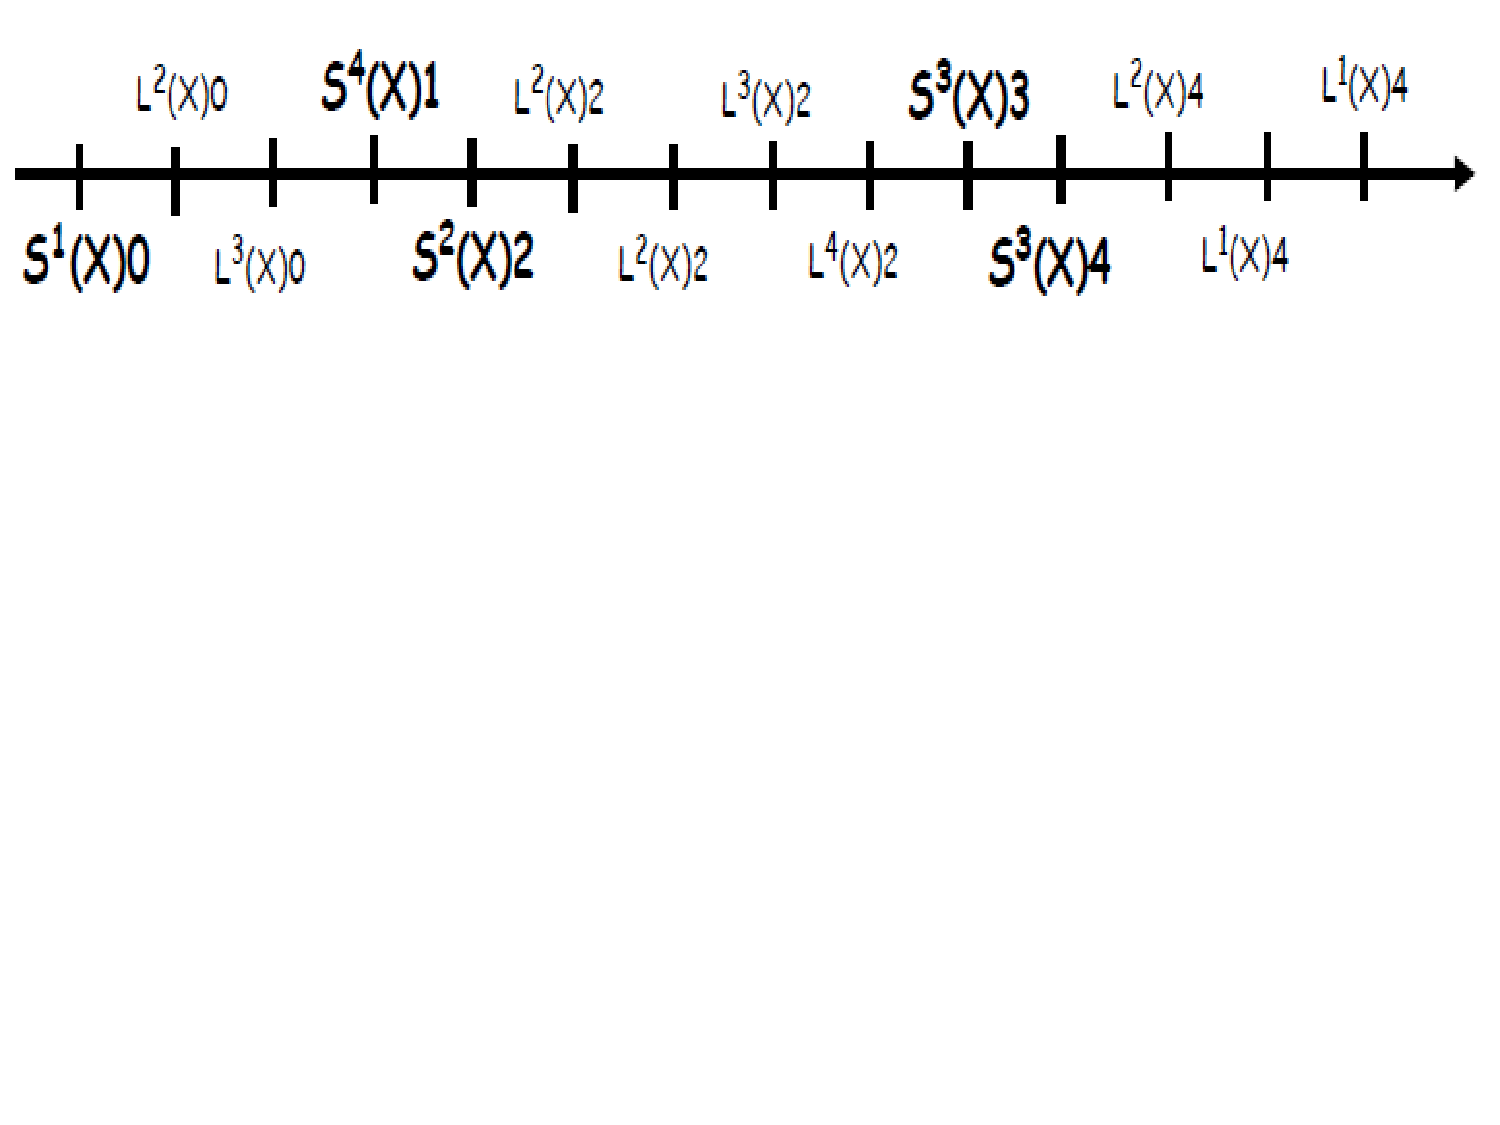
\includegraphics[width=55ex]{Ch7Figs/CoherenceEG2}\vspace{-30ex}
    
    \item Since all accesses to every location are in thread order and every
            load returns the value of the latest store in the (choosen) order,
            one can schedule accesses one by one on the formal model and
            obtain the same values return by all loads. %the execution above is plain coherent! 

\end{itemize}

\end{frame}


\begin{frame}[fragile,t]
\frametitle{Plain Coherence: Forwarding Store Buffers}

To prove a plain coherence, need to find a serial order of all mem accesses for 
all possible executions. Infinite $\Rightarrow$ Intractable.\medskip

\emph{Hardware built such that it constrains the possible executions and ensures 
a serial order is possible}.

\begin{columns}
\column{0.59\textwidth}
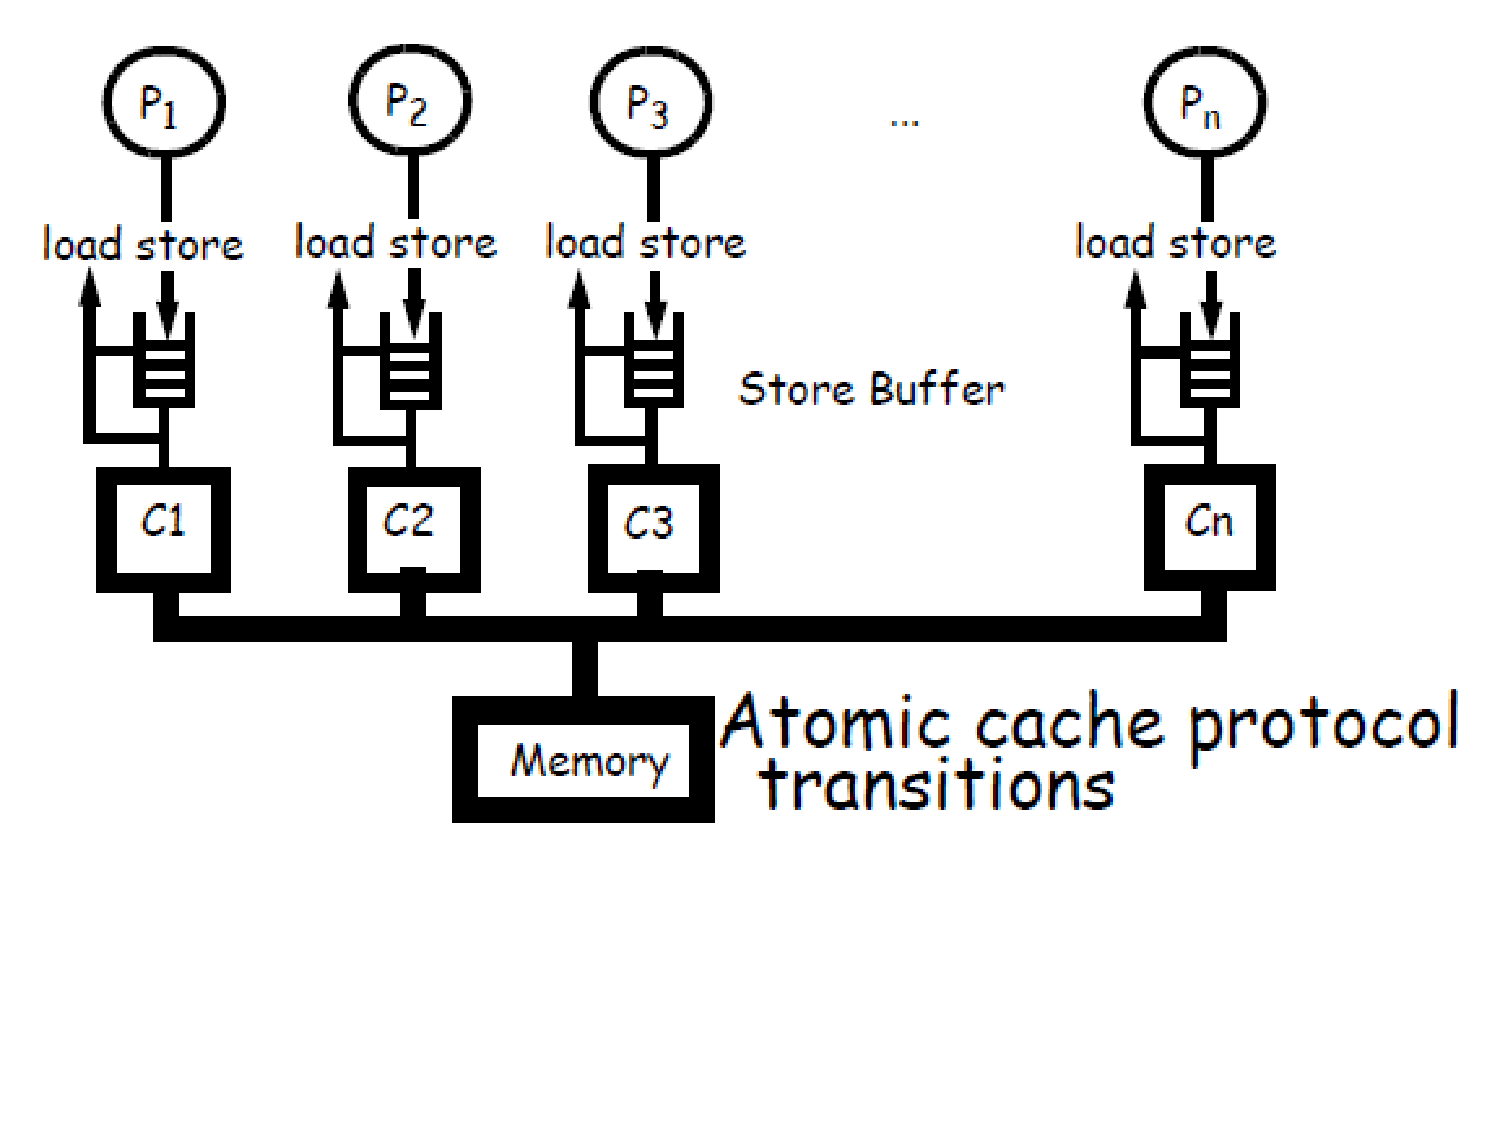
\includegraphics[width=44ex]{Ch7Figs/FwdStoreBuff}%\vspace{-30ex} 
\column{0.40\textwidth}
\vspace{-6ex}
\begin{itemize}
    \item \emp{Store buffer with forwarding is PLAIN coherent, but NOT store atomic!}
    \item Stores: inserted in store buffer and issued to cache later,
    \item Loads satisfied from store buffer if same address, else memory.
\end{itemize}
\end{columns}
\vspace{-3ex}
\alert{Store buffers not subject to the cache coherence protocol!}

\end{frame}

\begin{frame}[fragile,t]
\frametitle{Plain Coherence: Forwarding Store Buffers Example}
\vspace{-3ex}

{\center 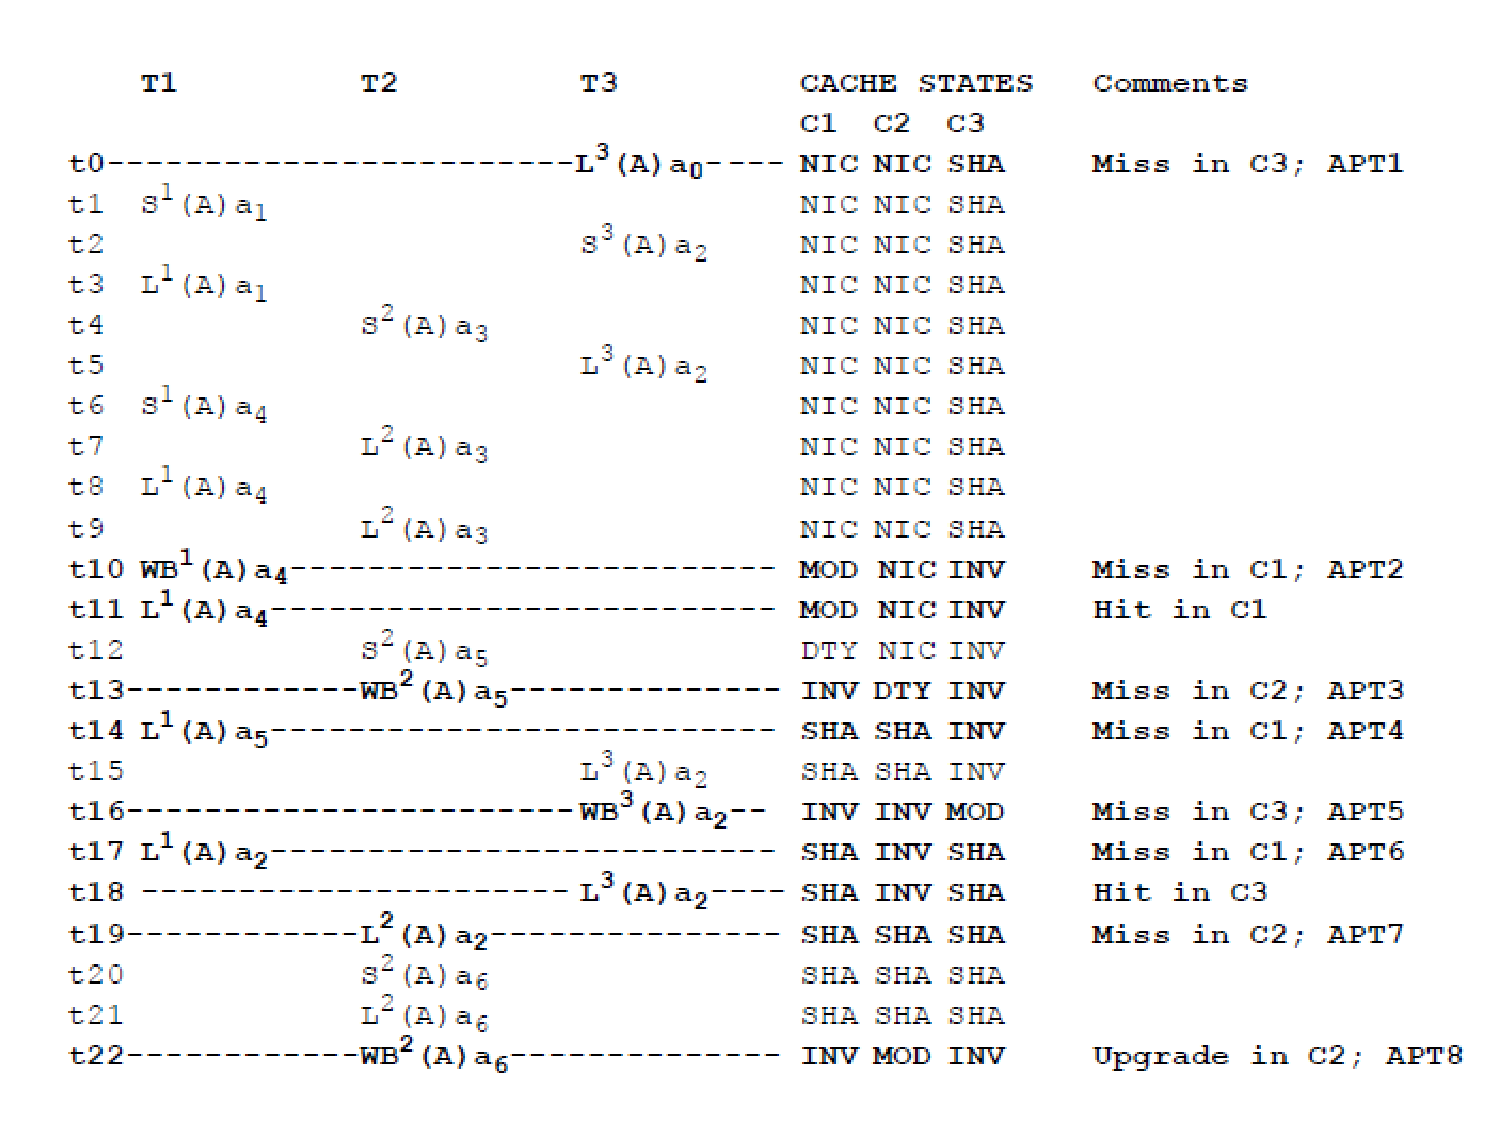
\includegraphics[width=65ex]{Ch7Figs/FwdStoreBuffEG1}}

\end{frame}

\begin{frame}[fragile,t]
\frametitle{Plain Coherence: Forwarding Store Buffers Example}

\begin{itemize}
    \item Aggressive Store Buffer:
        \begin{itemize}
            \item Stores overwrite previous same-address values in SB, 
%                    i.e., single value per address in SB,
            \item stores forward values to loads.
        \end  {itemize}

    \item The backbone of the global order are the GP accesses, i.e.,
            the ones atomically executed in cache:\\
            {\tt{}INIT$\rightarrow$L$^3$(A)a$_0$$\rightarrow$WB$^1$(A)a$_4$$\rightarrow$L$^1$(A)a$_4$ $\rightarrow$WB$^2$(A)a$_5$$\rightarrow$ L$^1$(A)a$_5$}\\
            {\tt~~~~$\rightarrow$WB$^3$(A)a$_2$$\rightarrow$ L$^1$(A)a$_2$$\rightarrow$L$^3$(A)a$_2$$\rightarrow$L$^2$(A)a$_2$$\rightarrow$WB$^2$(A)a$_6$}\medskip

    \item We then expand all write buffer (WB) by local load/stores:\\
           {\tt{}INIT$\rightarrow$L$^3$(A)a$_0$$\rightarrow$S$^1$(A)a$_1$$\rightarrow$L$^1$(A)a$_1$$\rightarrow$S$^1$(A)a$_4$$\rightarrow$L$^1$(A)a$_4$$\rightarrow$L$^1$(A)a$_4$}\\
           {\tt~~~~$\rightarrow$S$^2$(A)a$_3$$\rightarrow$L$^2$(A)a$_3$$\rightarrow$L$^2$(A)a$_3$$\rightarrow$S$^2$(A)a$_5$$\rightarrow$L$^1$(A)a$_5$$\rightarrow$S$^3$(A)a$_2$}\\
           {\tt~~~~$\rightarrow$L$^3$(A)a$_2$$\rightarrow$L$^3$(A)a$_2$$\rightarrow$L$^1$(A)a$_2$$\rightarrow$L$^3$(A)a$_2$$\rightarrow$L$^2$(A)a$_2$$\rightarrow$S$^2$(A)a$_6$}\\ 
           {\tt~~~~$\rightarrow$L$^2$(A)a$_6$}\medskip

    \item Temporal order: {\tt~a$_0\rightarrow$a$_1\rightarrow$a$_2\rightarrow$a$_3\rightarrow$a$_4\rightarrow$a$_5\rightarrow$a$_6$}
    \item Coherence order: {\tt a$_0\rightarrow$a$_1\rightarrow$a$_4\rightarrow$a$_3\rightarrow$a$_5\rightarrow$a$_2\rightarrow$a$_6$}
    \item P1 observes: {\tt a$_1\rightarrow$a$_4\rightarrow$a$_5\rightarrow$a$_2$}
    \item P2 observes: {\tt a$_3\rightarrow$a$_5\rightarrow$a$_2\rightarrow$a$_6$~} and 
    P3 observes: {\tt a$_0\rightarrow$a$_2$}

\end{itemize}


\end{frame}


\begin{frame}[fragile,t]
\frametitle{Generalizations}

\begin{itemize}
    \item \emp{``Privacy Principle''}: a thread may access its own
            private values, which are not propagated to other threads,
            without violating coherence.
        \begin{itemize}
            \item The reason is that no other order can observe the
                    values, so it is ``easy'' to insert accesses to them in a global order.
        \end  {itemize}\bigskip

    \item This result can be generalized:
        \begin{itemize}
            \item Other store buffer management (recombining: the most aggressive),
            \item In lock-up free caches, a block can be allocated on a store miss,
                    filled by a store while the miss is pending and the stored value
                    can be read by a thread.
            \item Threads in MT cores can reach other's values in L1, while the miss is pending,
            \item Clusters of procs running many threads may share pending values in shared buffers.
            \item A thread may modify and use the value returned by a directory
                    protocol even before invalidations are executed (early ack).
        \end  {itemize}\bigskip

\end{itemize}


\end{frame}


\begin{frame}[fragile,t]
\frametitle{Is There Any Non-Coherent Execution?}

\begin{columns}
\column{0.59\textwidth}
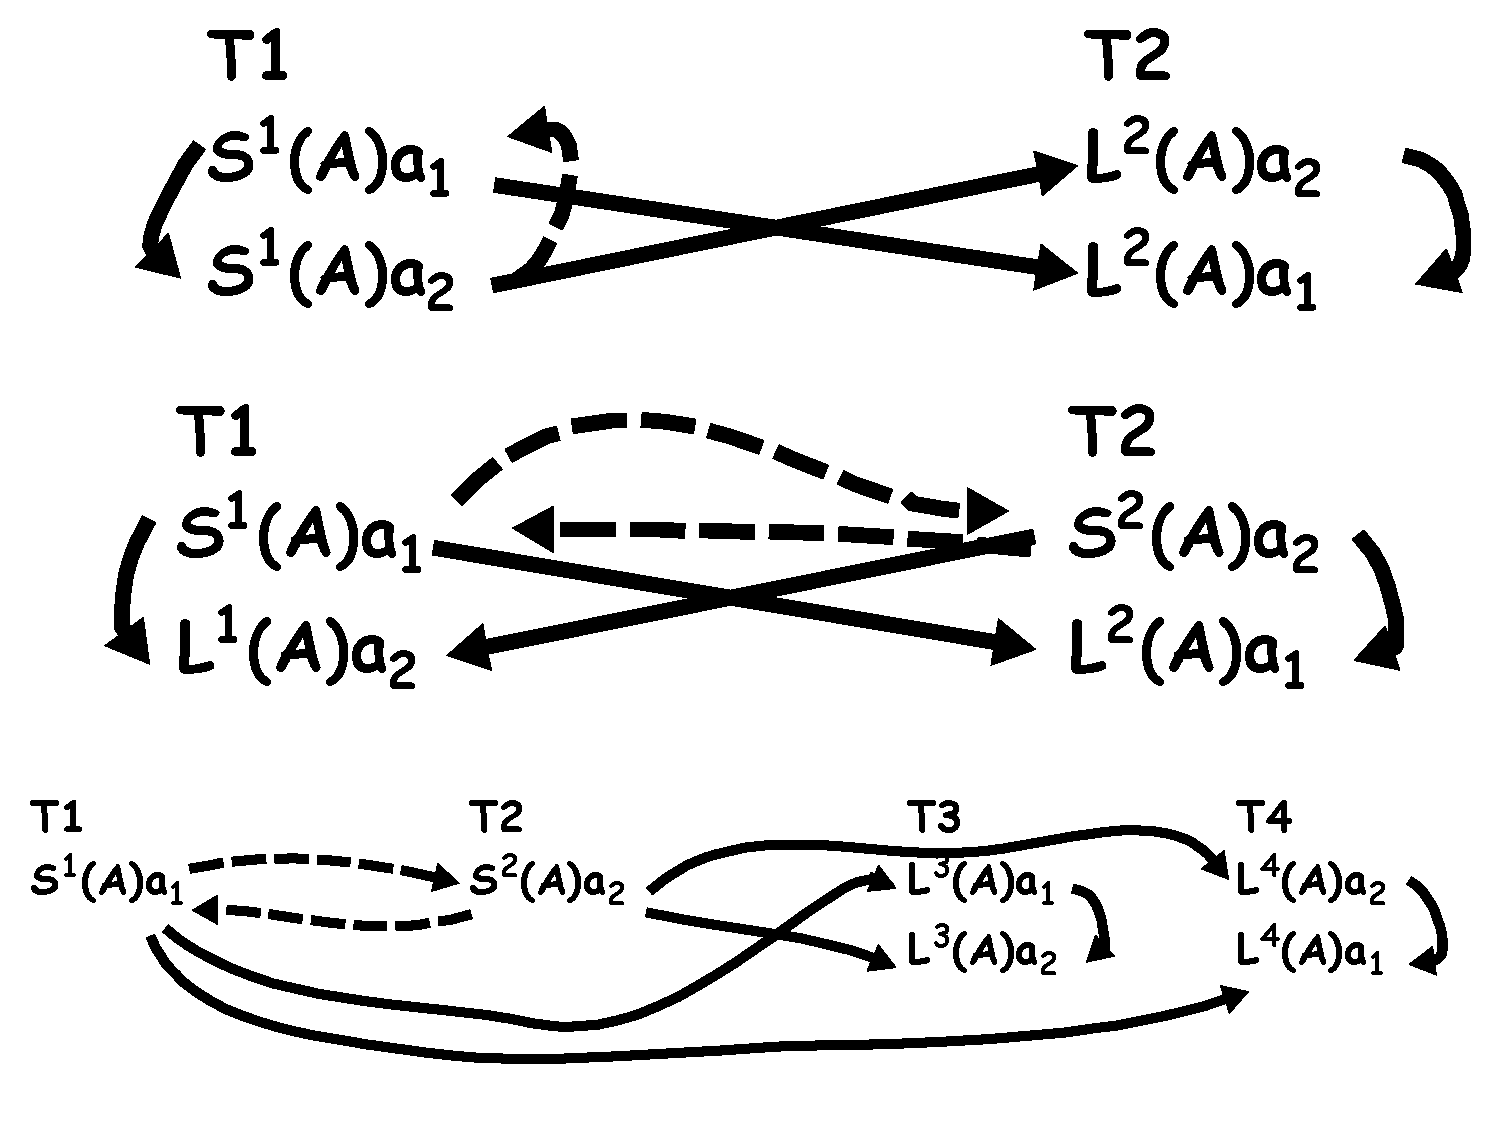
\includegraphics[width=44ex]{Ch7Figs/NonCoherentExecs}%\vspace{-30ex} 
\column{0.46\textwidth}

\begin{itemize}
    \item[1] A thread observes two stores of another thread out of order.
    \item[2] Threads observe each other's stores instead of their own,
    \item[3] two stores in different threads are not ordered, but are 
                observed in different orders by two separate threads.
\end{itemize}
\end{columns}
\bigskip

\alert{The execution is NOT coherent in any of the three cases, because
stores to the same variable cannot be observed in different orders.}

\end{frame}

\begin{frame}[fragile,t]
\frametitle{Importance of Coherence}

\begin{itemize}
    \item Coherence seems a very weak property, but
    \item it is extremely useful because:\medskip
    \begin{itemize}
        \item[1] guarantees that stores to the same location are ordered,\medskip
        \item[2] it facilitates the implementation of memory consistency
                    models (next)\medskip
        \item[3] ensures that if the computation is interrupted, the memory
                    system converges to a consistent state for all data
                    (after all in-progress instrs terminate \& nrtwork 
                    and buffers are drained)\medskip
        \item[4] for example it enables thread migration.
    \end{itemize}

\end{itemize}

\end{frame}

\subsection{Problems With Plain Coherence}

\begin{frame}[fragile,t]
\frametitle{The Problem With Plain Coherence}

\begin{itemize}
    \item Plain Coherence is NOT composable  with other possible orders: 
    \begin{itemize}
        \item[1] load-load or load-store on different locations,
        \item[2] inter-thread synchronizations
        \item[3] lock, barrier atomic instructions (synchronization)\medskip
    \end{itemize}
\end{itemize}


\begin{columns}
\column{0.47\textwidth}
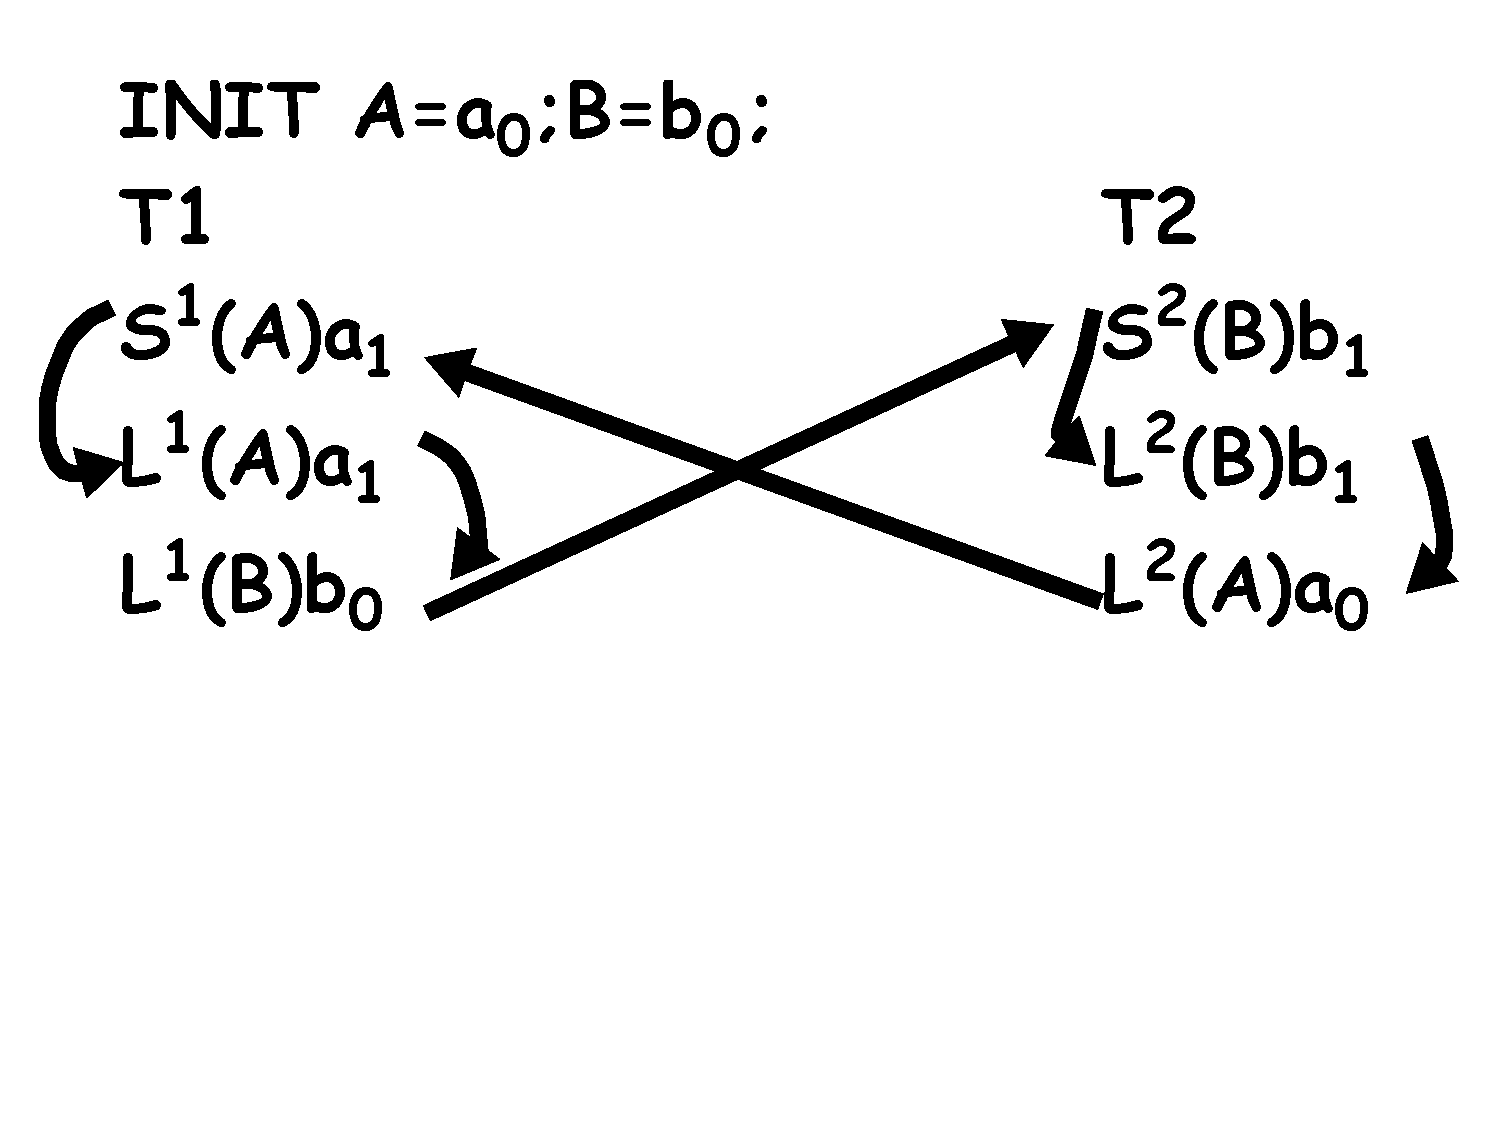
\includegraphics[width=38ex]{Ch7Figs/ProblemPlainCoh}
\column{0.50\textwidth}
\vspace{-7ex}
\begin{itemize}
    \item[1] Plain Coherent Accesses on {\tt A}:\\
                {\tt L$^2$(A)a$_0\rightarrow$S$^1$(A)a$_1\rightarrow$L$^1$(A)a$_1$}
    \item[2] Plain Coherent Accesses on {\tt B}:\\
                {\tt L$^1$(B)b$_0\rightarrow$S$^2$(B)b$_1\rightarrow$L$^2$(B)b$_1$}
    \item[3] \alert{But no interleaving of accesses can give that result}. 
\end{itemize}
\end{columns}
\vspace{-7ex}

\begin{itemize}
    \item The reason is that plain coherence order $\neq$ temporal order.
    \item When global order does not exist, it is difficult to construct
            an intuitive \& useful semantics.\medskip
\end{itemize}

\emph{However, we can build on top of store atomicity!}

\end{frame}


\begin{frame}[fragile,t]
\frametitle{Why Coherence Is Not Sufficient (?) Examples}

\begin{block}{Communication{\tt~~~~~~~~~~~~~~~~~~} Point-to-Point Synchronization}
\begin{columns}
\column{0.18\textwidth}
\begin{colorcode}[fontsize=\scriptsize]
    INIT: A := B := 0
//P1
...
A := 1
B := 2
// Impossible to print (B=2, A=0)
\end{colorcode} 
\column{0.18\textwidth}
\begin{colorcode}[fontsize=\scriptsize]

//P2
...
print B
print A

\end{colorcode} 
\column{0.18\textwidth}
\begin{colorcode}[fontsize=\scriptsize]
    INIT: A := FLAG := 0
P1
...
A    := 1;
FLAG := 1;
//Impossible to print (A=0)
\end{colorcode} 
\column{0.25\textwidth}
\begin{colorcode}[fontsize=\scriptsize]

P2
...
while( FLAG == 0 ) ;
print A

\end{colorcode} 
\end{columns}
\end{block}

\begin{block}{Dekker's Algorithm Simplified}
\begin{columns}
\column{0.18\textwidth}\vspace{-2ex}
\begin{colorcode}[fontsize=\scriptsize]
    INIT: A := B := 0
//P1
...
A := 1
print B;
// Impossible to print (B=0, A=0)
\end{colorcode} 
\column{0.18\textwidth}\vspace{-2ex}
\begin{colorcode}[fontsize=\scriptsize]

//P2
B := 1
print A

\end{colorcode} 
\column{0.57\textwidth}\vspace{-2ex}
\begin{itemize}
    \item Programmer's intuition is that accesses from different processes are 
            ``interleaved'' in process order.
    \item Plain coherence is satisfied, for each memory location individually,
            but result does not make sense!
\end{itemize}
\end{columns}
\end{block}


\emp{Need Sequential Consistency for Different Memory Accesses.}

\end{frame}


%%%%%%%%%%%%%%%%%%%%%%%%%%%%%%%%%%%%%%%%%%%%
%%%%%%%%%%%%%%%%%%%%%%%%%%%%%%%%%%%%%%%%%%%%
%%%%%%%%%%%%%%%%%%%%%%%%%%%%%%%%%%%%%%%%%%%%
\section{Sequential Consistency}

\begin{frame}[fragile]
	\tableofcontents[currentsection]
\end{frame}

\subsection{General Case}

\begin{frame}[fragile,t]
\frametitle{Formal Model For Sequential Consistency (SC)}

{\center 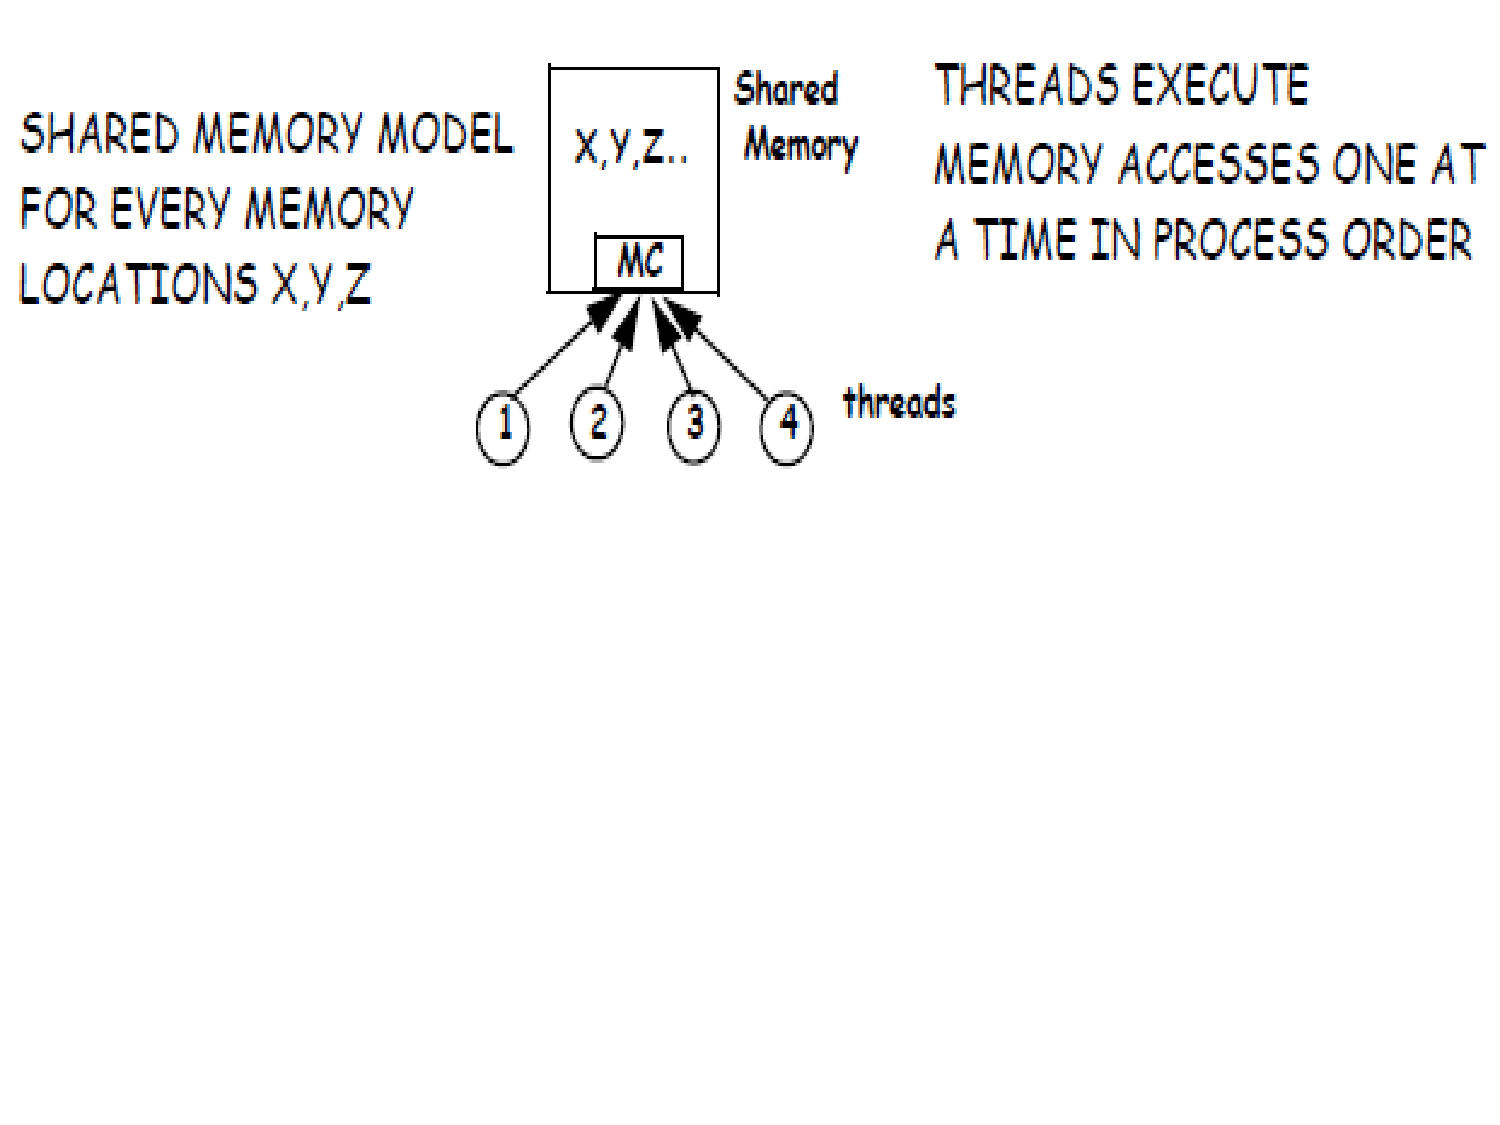
\includegraphics[width=59ex]{Ch7Figs/MemSeqCons}}\pause
\vspace{-20ex}

\begin{itemize}
    \item Program order of all threads is respected and all memory accesses are atomic
            because of the memory controller.
    \begin{itemize}
        \item \emp{\bf ``A multiprocessor is sequential consistent if the RESULT of ANY
                execution is the same AS IF the memory operations of all processors
                were executed in SOME sequential order and the operations of each
                individual processor appear in the order specified by the program.''}
    \end  {itemize}
\end{itemize}

\end{frame}

\begin{frame}[fragile,t]
\frametitle{Formal Model For Sequential Consistency (SC)}

\begin{block}{We take a look at AS IF:}
\begin{columns}
\column{0.18\textwidth}\vspace{-2ex}
\begin{colorcode}[fontsize=\scriptsize]
        INIT: A := B := 0
//P1
A := 1;
B := 2;
// POSSIBLE: (A,B)=(0,0),(1,0),(1,2)
\end{colorcode} 
\column{0.18\textwidth}\vspace{-2ex}
\begin{colorcode}[fontsize=\scriptsize]

//P2
print B
print A

\end{colorcode} 
\end{columns}
\end{block}

\begin{itemize}
    \item \alert{IMPOSSIBLE under SC: (0,2)}\bigskip
    \item \emph{Execution {\tt B := 2 $\rightarrow$ A := 1$ \rightarrow$ print A $\rightarrow$ print B}}:    
    \begin{itemize}
        \item same result as {\tt A := 1 $\rightarrow$ B := 2 $\rightarrow$ print B $\rightarrow$ print A}\medskip
        \item \emph{is SC even if the temporal order violates the process order!}
    \end  {itemize}\bigskip

    \item \emp{As for coherence, SC order is not necessarily temporal order!}
\end{itemize}

\end{frame}


\begin{frame}[fragile,t]
\frametitle{Sequential Consistency (SC): Orders \& Hardware}

\begin{columns}
\column{0.55\textwidth}
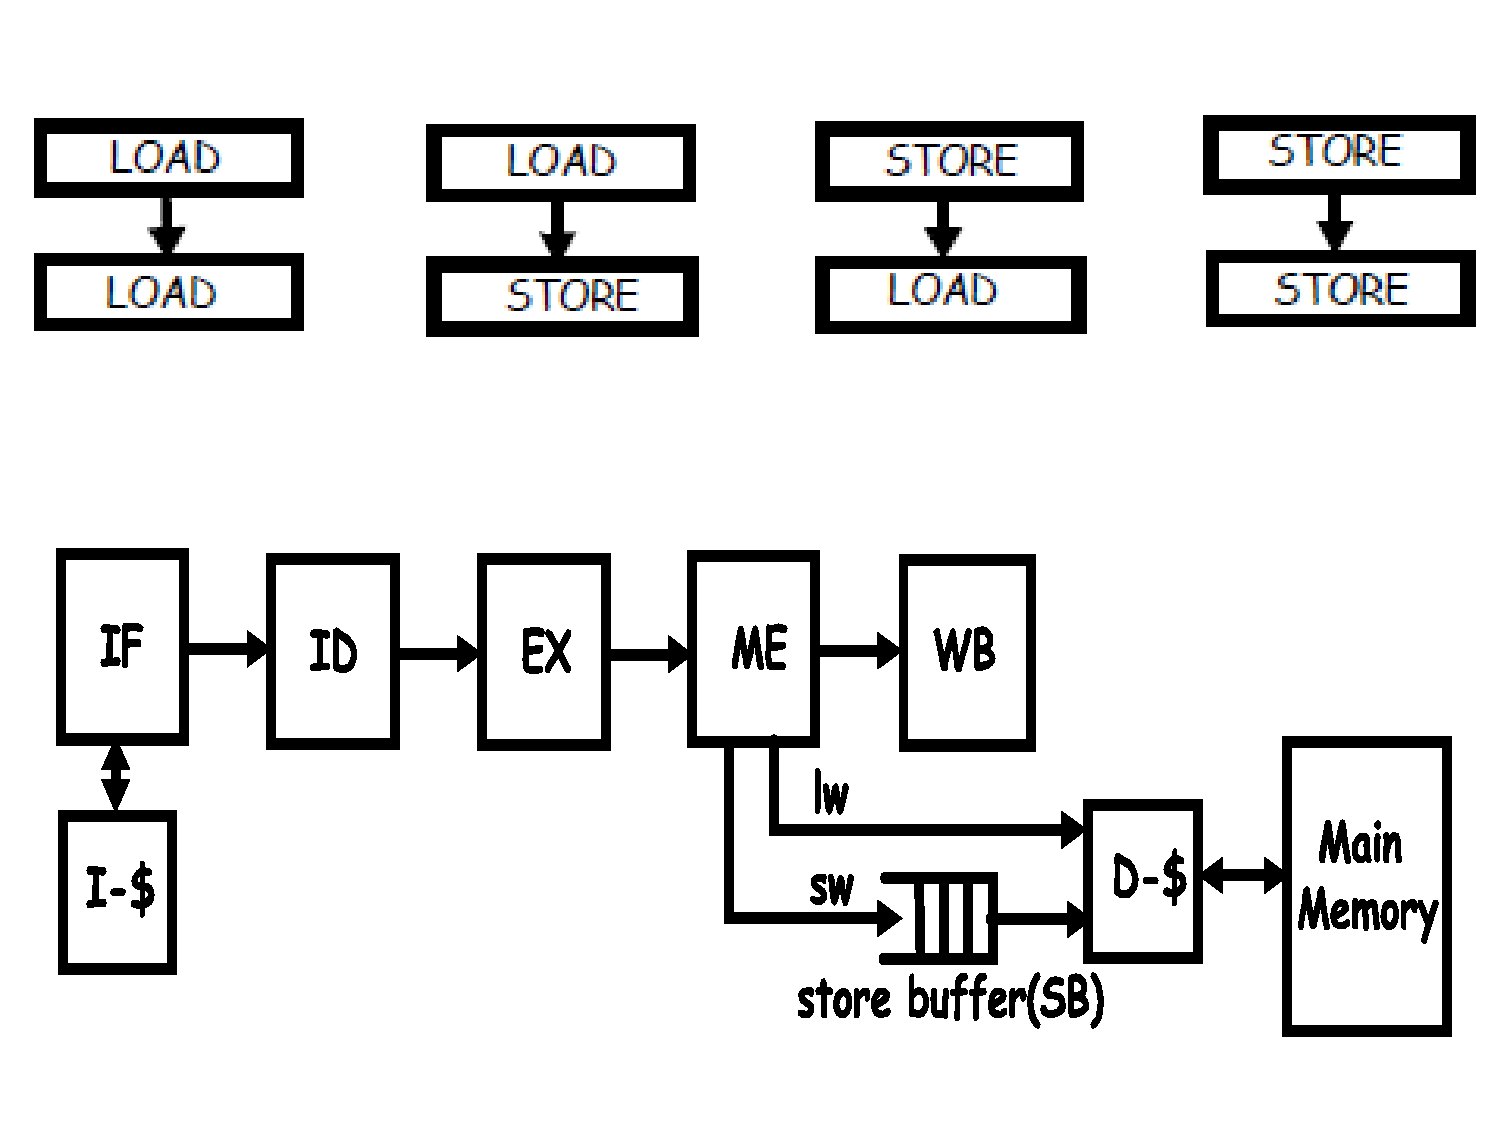
\includegraphics[width=44ex]{Ch7Figs/OrdersPipeline}
\column{0.4\textwidth}
\begin{itemize}
    \item all memory orders must be enforced (globally performed GP)
    \item If memory is atomic, i.e., only GP loads can return values,
            what does it means for IO processors?
\end{itemize}
\end{columns}

\begin{itemize}
    \item Loads are blocking: load-load and load-store orders enforced.
    \item Stores are non-blocking (they move to SB)
    \begin{itemize}
        \item \emp{store-load:} loads must block in ME until SB is empty,
        \item \emp{store-store:} stores must be GPed one by one from SB
    \end{itemize} 
\end{itemize}
\end{frame}

\begin{frame}[fragile,t]
\frametitle{Sufficient Conditions for SC}

\emp{\bf Need to find a total coherent order of ALL MEMORY
ACCESSES such that intra-thread accesses are in thread order 
for any execution}.
\begin{itemize}
    \item simply schedule each access one at a time on the formal model
    \item \emph{Sufficient Condition:} every processor globally performs
                its memory accesses in thread order.
\end{itemize}
\bigskip

In Sequential-Consistency Order:
\begin{itemize}
    \item[1] accesses to all locations from each thread must be in thread order
    \item[2] source (store) of value must precede the load of the value
    \item[3] implied rule: there can be no store between the store sourcing the 
                value and the load reading the value
\end{itemize}

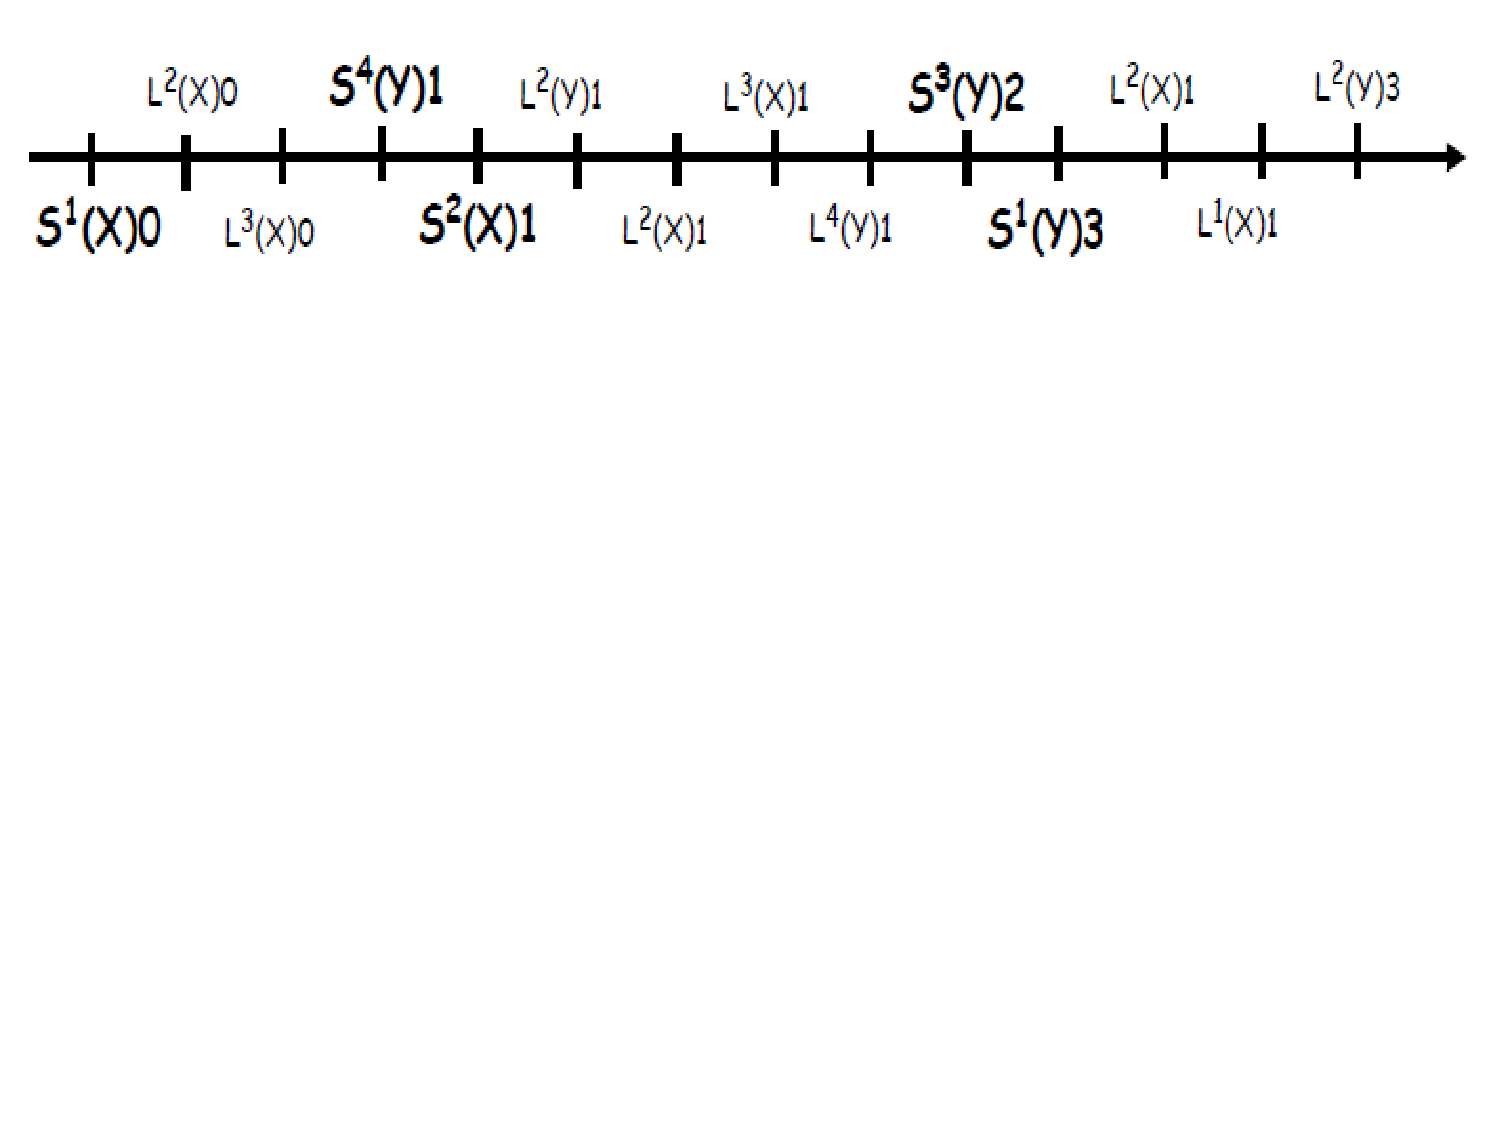
\includegraphics[width=59ex]{Ch7Figs/EqSeqConst}

\end{frame}


\begin{frame}[fragile,t]
\frametitle{Sequential Consistency: Store Buffers Problems}

\emp{\bf With Store Buffers, loads can be GPed before previous stores:}
\begin{itemize}
    \item in SC a load must be stalled if prior stores are not GPed
    \item \emph{effective for long bursts of store}, but still stores must
                be propagated one by one.
\end{itemize}
\bigskip

\begin{columns}
\column{0.18\textwidth}\vspace{-10ex}
\begin{colorcode}[fontsize=\scriptsize]
// Intially, A and B are 0 
// and are cached as Shared 
//P1
S\mymath{\myindu{1}}(A)1
L\mymath{\myindu{1}}(B)0
\end{colorcode} 
\column{0.18\textwidth}\vspace{-10ex}
\begin{colorcode}[fontsize=\scriptsize]


//P2
S\mymath{\myindu{2}}(B)1
L\mymath{\myindu{2}}(A)0
\end{colorcode} 
\column{0.60\textwidth}
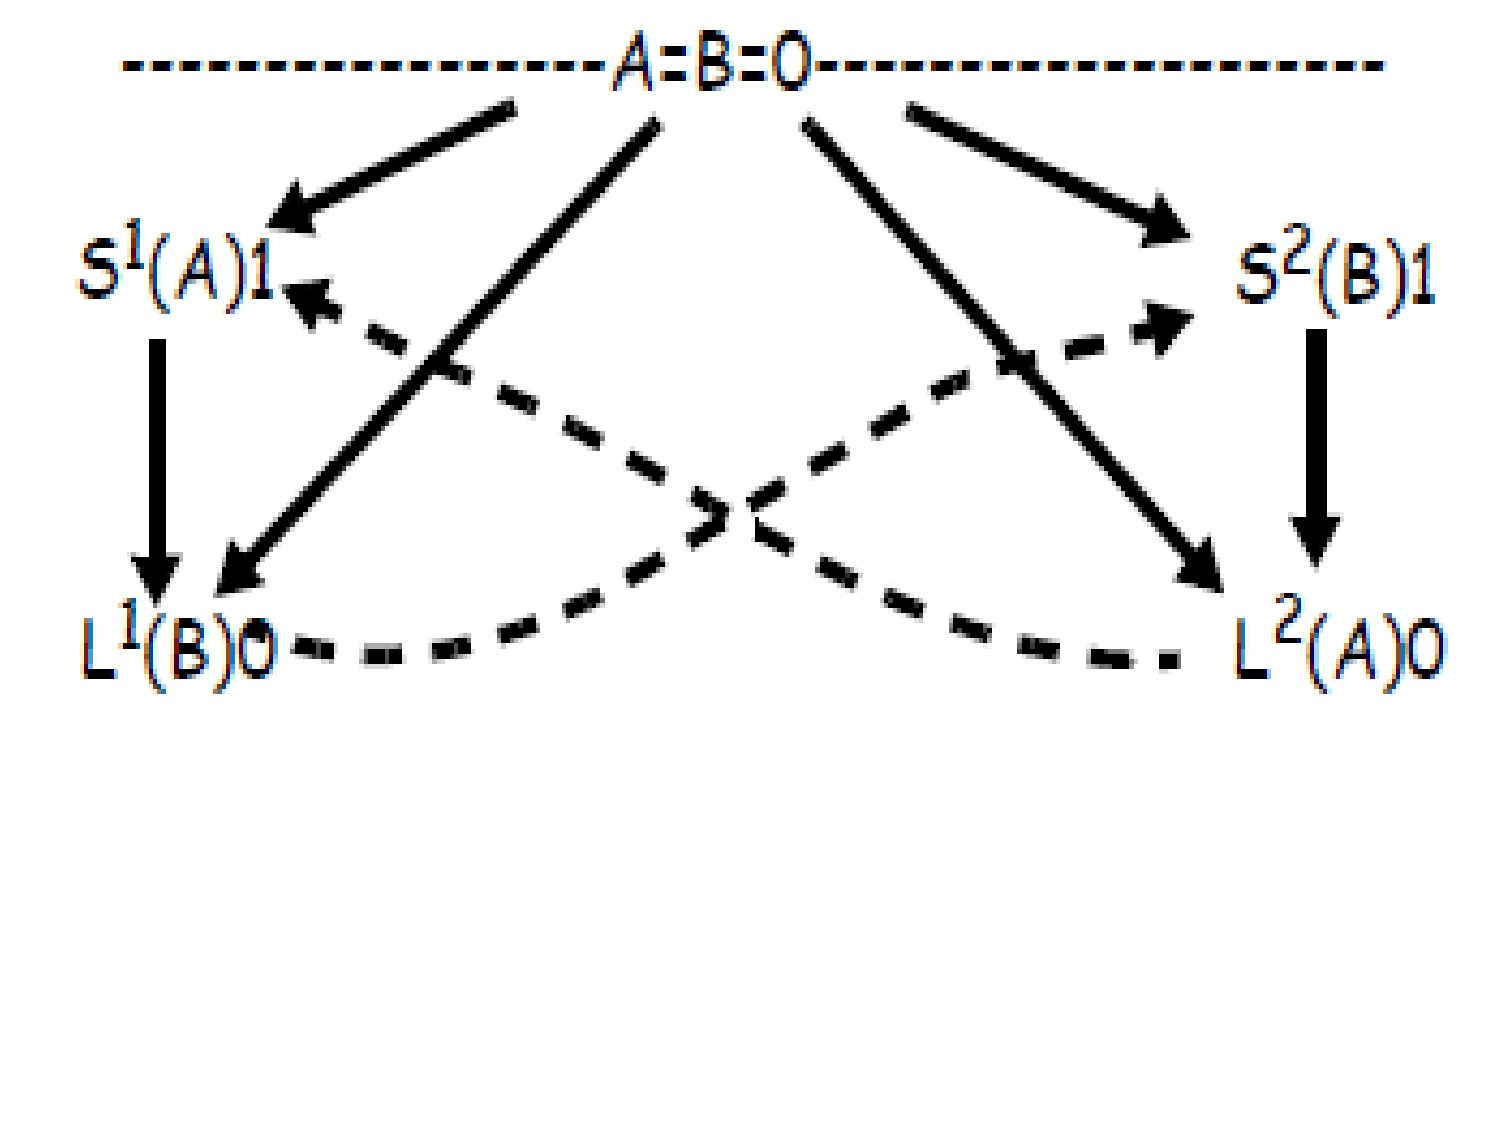
\includegraphics[width=39ex]{Ch7Figs/SeqConsGraphEg}
\end{columns}
\vspace{-8ex}

\alert{Execution Graph Has Cycles $\Rightarrow$ Execution Cannot be Ordered}:
\begin{itemize}
    \item with store buffers, the outcome can be {\tt (0,0)}
    \item P1 executes {\tt A:=1;} which stays in store buffer, similar for P2
    \item \alert{P1 and P2 can both read 0 before (MSI) invalidation occurs!}
\end{itemize}


\end{frame}


\begin{frame}[fragile,t]
\frametitle{Sequential Consistency Conclusions}

\begin{itemize}
    \item \emp{Sequential Consistency cannot take advantage of store buffers.}\medskip
    \item \emp{Also problems with compilers:}
\end{itemize}

\begin{block}{Point-to-Point Synchronization}
\begin{columns}
\column{0.23\textwidth}
\begin{colorcode}[fontsize=\scriptsize]
        INIT: A := B := 0
//P1
...
A    := 1;
FLAG := 1;
...
\end{colorcode} 
\column{0.23\textwidth}
\begin{colorcode}[fontsize=\scriptsize]

//P1
...
while ( FALG == 0 ) ;
print(A);
...
\end{colorcode} 
\column{0.45\textwidth}
\begin{itemize}
    \item There is no dependency between {\tt FLAG} and {tt A} $\Rightarrow$\smallskip
    \item \emp{Compiler may reorder instructions in {\tt P1}}
    \item \alert{Compiler may even remove the {\tt while} loop!}
    \item use of \emph{\tt volatile}.
\end  {itemize}
\end{columns}
\end{block}
\bigskip

\emph{Bend the Rules Again: Memory Consistency Models} implement a 
tradeoff between performance and ease of use (user intuition).

\end{frame}

\subsection{Memory Consistency Models}

\begin{frame}[fragile,t]
\frametitle{Memory Consistency Models}

Any other programmer intuition that we may exploit?

Explicit Synchronization (still expensive):

\begin{columns}
\column{0.2\textwidth}
\begin{colorcode}[fontsize=\scriptsize]
        INIT: BAR := 0
//P1
A := 1;
B := 2;
BARRIER(BAR,2);
\end{colorcode} 
\column{0.2\textwidth}
\begin{colorcode}[fontsize=\scriptsize]

//P1
BARRIER(BAR,2);
R1 := A;
R2 := B;
\end{colorcode} 
\column{0.5\textwidth}
\begin{itemize}
    \item When shared, access to variables protected by locks. 
    \item Because of the barrier the result is always SC.
\end  {itemize}
\end{columns}
\bigskip

\emp{Should we care about programmer at all?} E.g.,
hardware-friendly memory-access ordering rules constraining what
programmer can do.
\medskip

Need an agreement between programmers (intuitive model) 
and hardware architects (performance)! 
\medskip

\emph{Memory Consistency Model is the interface between hardware and software \& 
should be/IS part of ISA Definition.}
\end{frame}


\begin{frame}[fragile,t]
\frametitle{Relaxed Memory Consistency Models}

\begin{columns}
\column{0.48\textwidth}
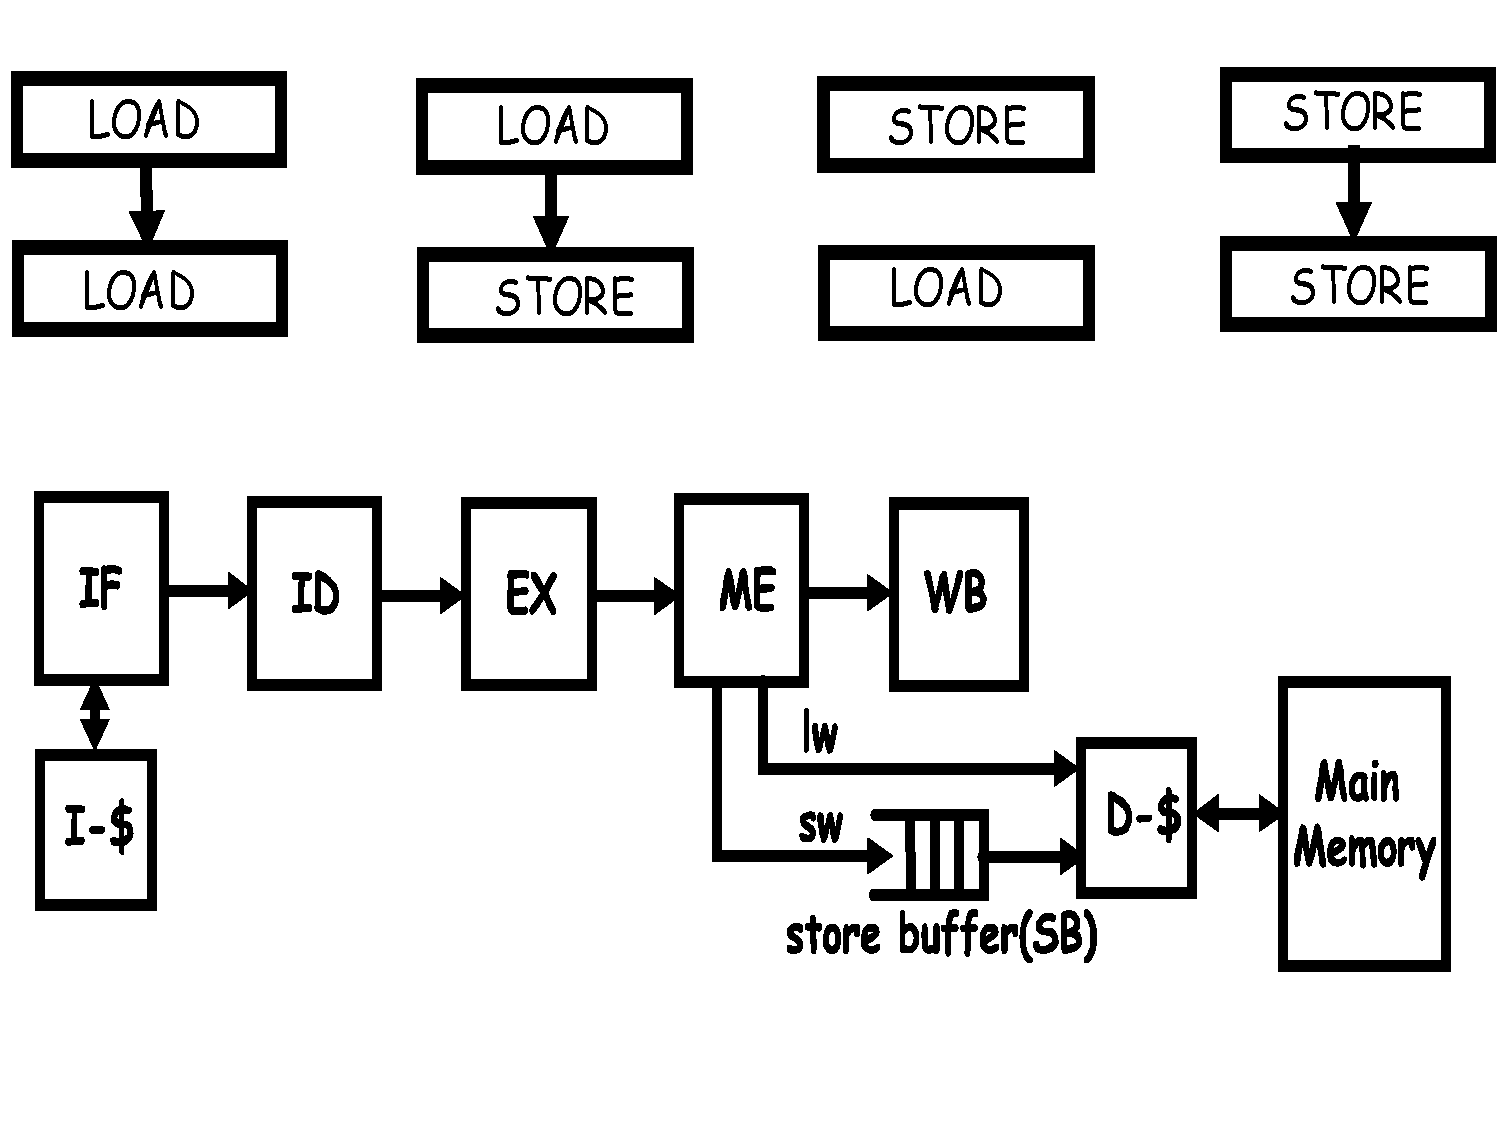
\includegraphics[width=39ex]{Ch7Figs/SeqConsRelatexOrders}\pause
\column{0.48\textwidth}
\begin{itemize}
    \item Relax some of the access orders of threads,e.g.,
    \item Processor View: memory is atomic, i.e., loads return 
            only (memory) GPed values,
    \item \emp{BUT loads are allowed to bypass stores (in buffer)!}
    \item {\tt store-loads} are not ordered $\Rightarrow$ 
            loads do not wait for store buffer to empty!  
\end{itemize}
\end{columns}
\bigskip

{\tt load$\rightarrow$load} {\tt store$\rightarrow$store} and {\tt load$\rightarrow$store}
performed by one processor still have to be observed in order by other procs, i.e., are ordered.

\end{frame}


\begin{frame}[fragile,t]
\frametitle{Relaxing Store-to-Load Orders}


\begin{columns}
\column{0.25\textwidth}
\begin{colorcode}[fontsize=\large]
  INIT: A := B := 0
//P1
A := 1;
print(B)
\end{colorcode} 
\column{0.25\textwidth}
\begin{colorcode}[fontsize=\large]

//P2
B := 1;
print(A);
\end{colorcode} 
\column{0.45\textwidth}
\alert{Remember This:\\Valid Execution\\May Print {\tt (0,0)}!}
\end{columns}
\bigskip

\begin{itemize}
    \item Example: Sun Micro Total Store Order (TSO)
        \begin{itemize}
            \item Dekker's algorithm does not work
            \item point-to-point communication still works.
        \end  {itemize}\smallskip

    \item Combining the stores in buffer {\em IFF} 
            no interleaved stores to different addresses.\smallskip

    \item Accesses to cache are submitted out of program order.\smallskip

    \item Values may or may not be forwarded from SB to loads:  
        \begin{itemize}
            \item no forwarding $\Rightarrow$ \emp{store atomic behavior}, but \alert{not coherent} 
                    (intra-thread dependencies not preserved)
            \item with forwarding $\Rightarrow$ plain coherence (a case of TSO),
                    i.e., some loads may return non-GPed values.  
        \end  {itemize}
\end{itemize}

\end{frame}


\begin{frame}[fragile,t]
\frametitle{TSO with No Forwarding}


\begin{columns}
\column{0.48\textwidth}
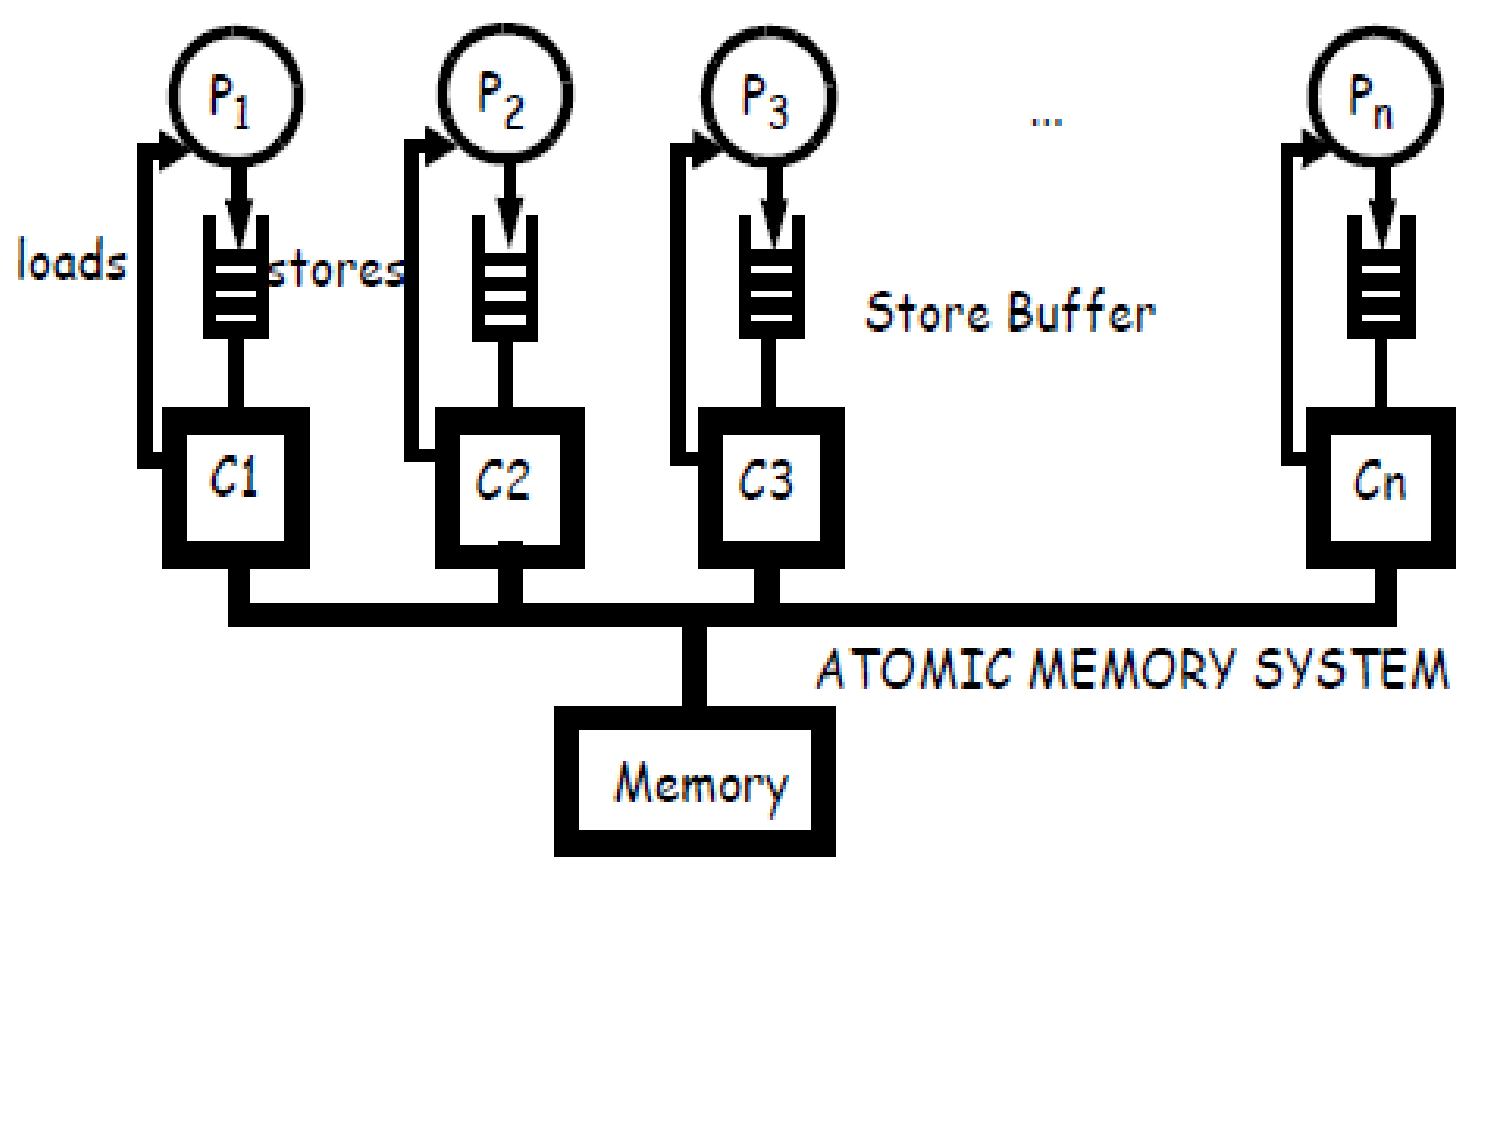
\includegraphics[width=39ex]{Ch7Figs/NoFwdingStoreBuf}\\\vspace{-5ex}
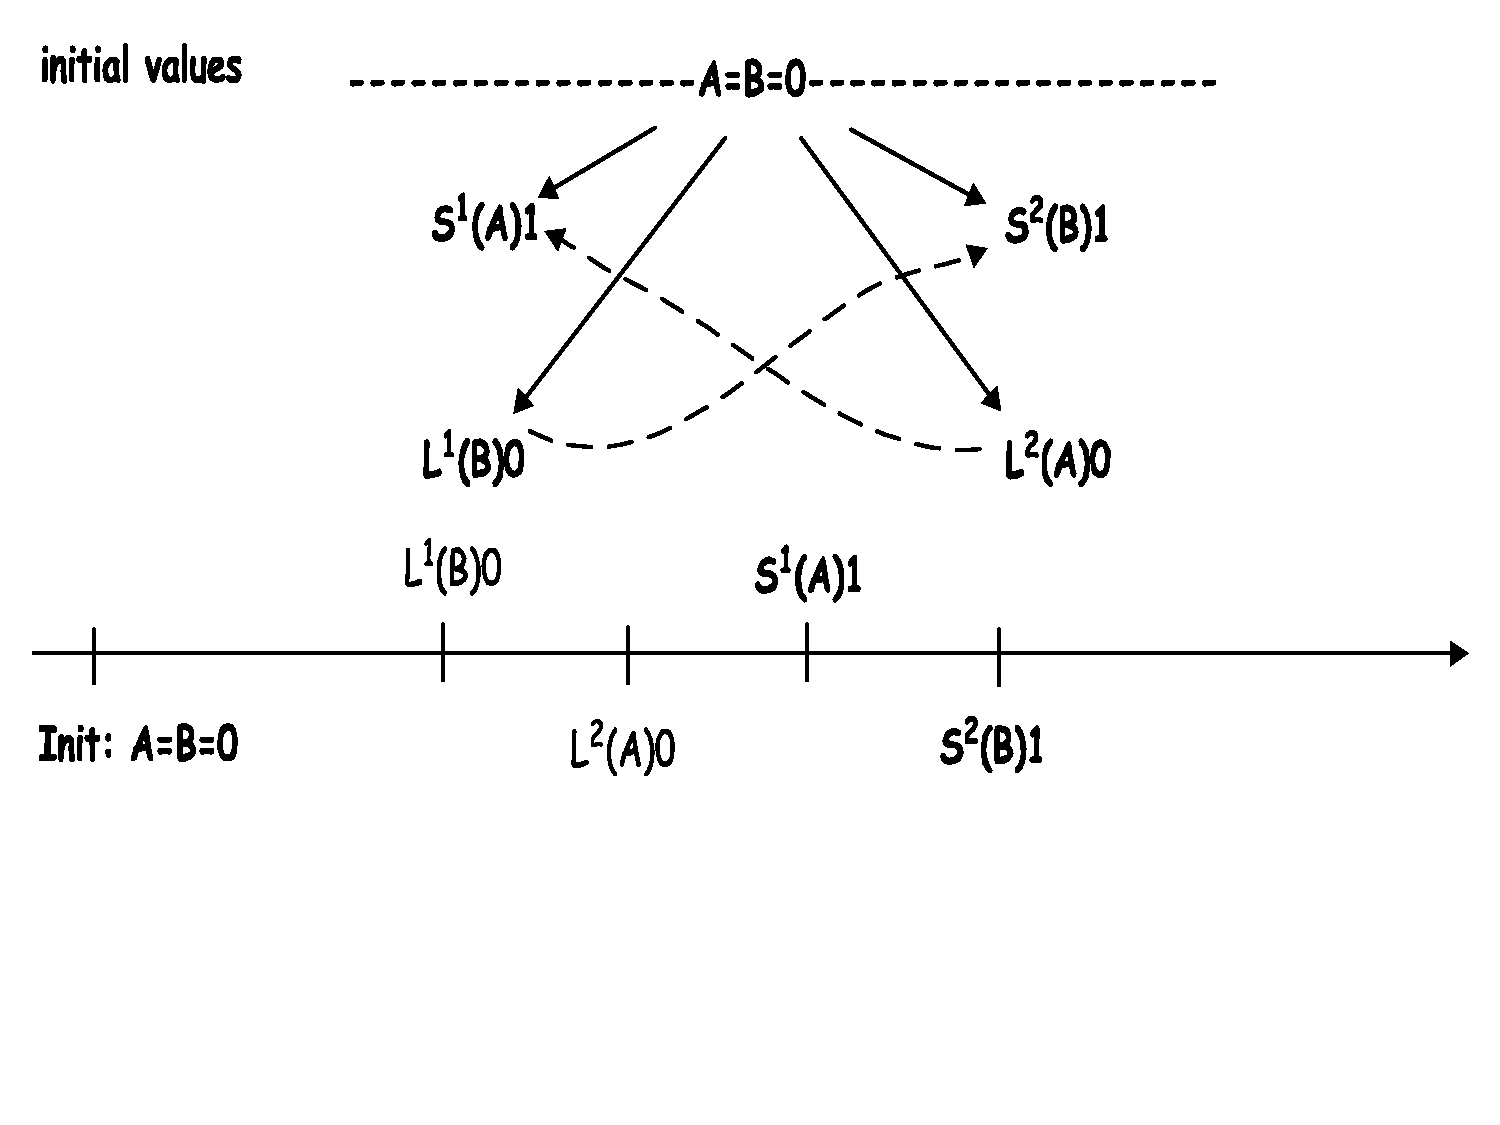
\includegraphics[width=39ex]{Ch7Figs/NoFwdingStoreBufGraph}\pause
\column{0.48\textwidth}
\vspace{-9ex}
\begin{itemize}
    \item Atomic stores; loads only returned GPed values.
    \item \alert{SB denotes the Private Store Pipeline} of the core, e.g., lockup-free cache.
    \item The Dekker's execution that fails to synchronize is VALID:
    \item no arrow between store and load in each thread $\Rightarrow$
    \item no global order between store and load
    \item still store is atomic overall, hence the order is valid under the model's rules.
\end{itemize}
\end{columns}
\end{frame}

\begin{frame}[fragile,t]
\frametitle{TSO With Forwarding}

\begin{columns}
\column{0.48\textwidth}
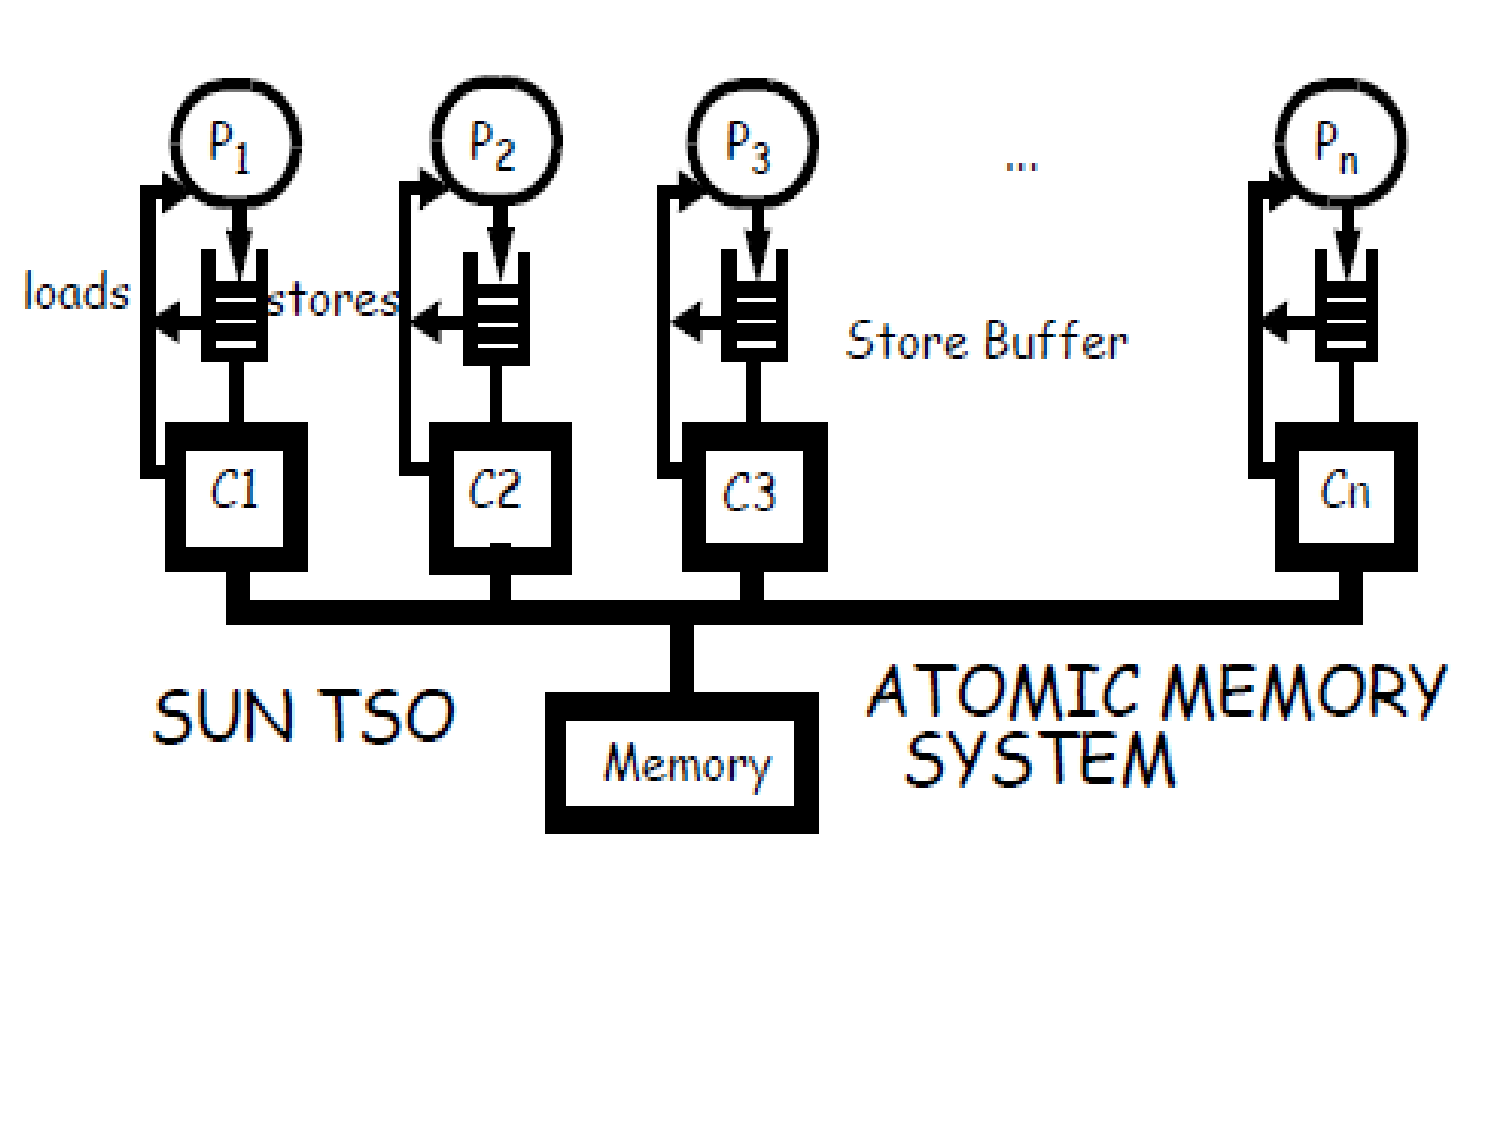
\includegraphics[width=39ex]{Ch7Figs/TSOfwd}\\\vspace{-5ex}
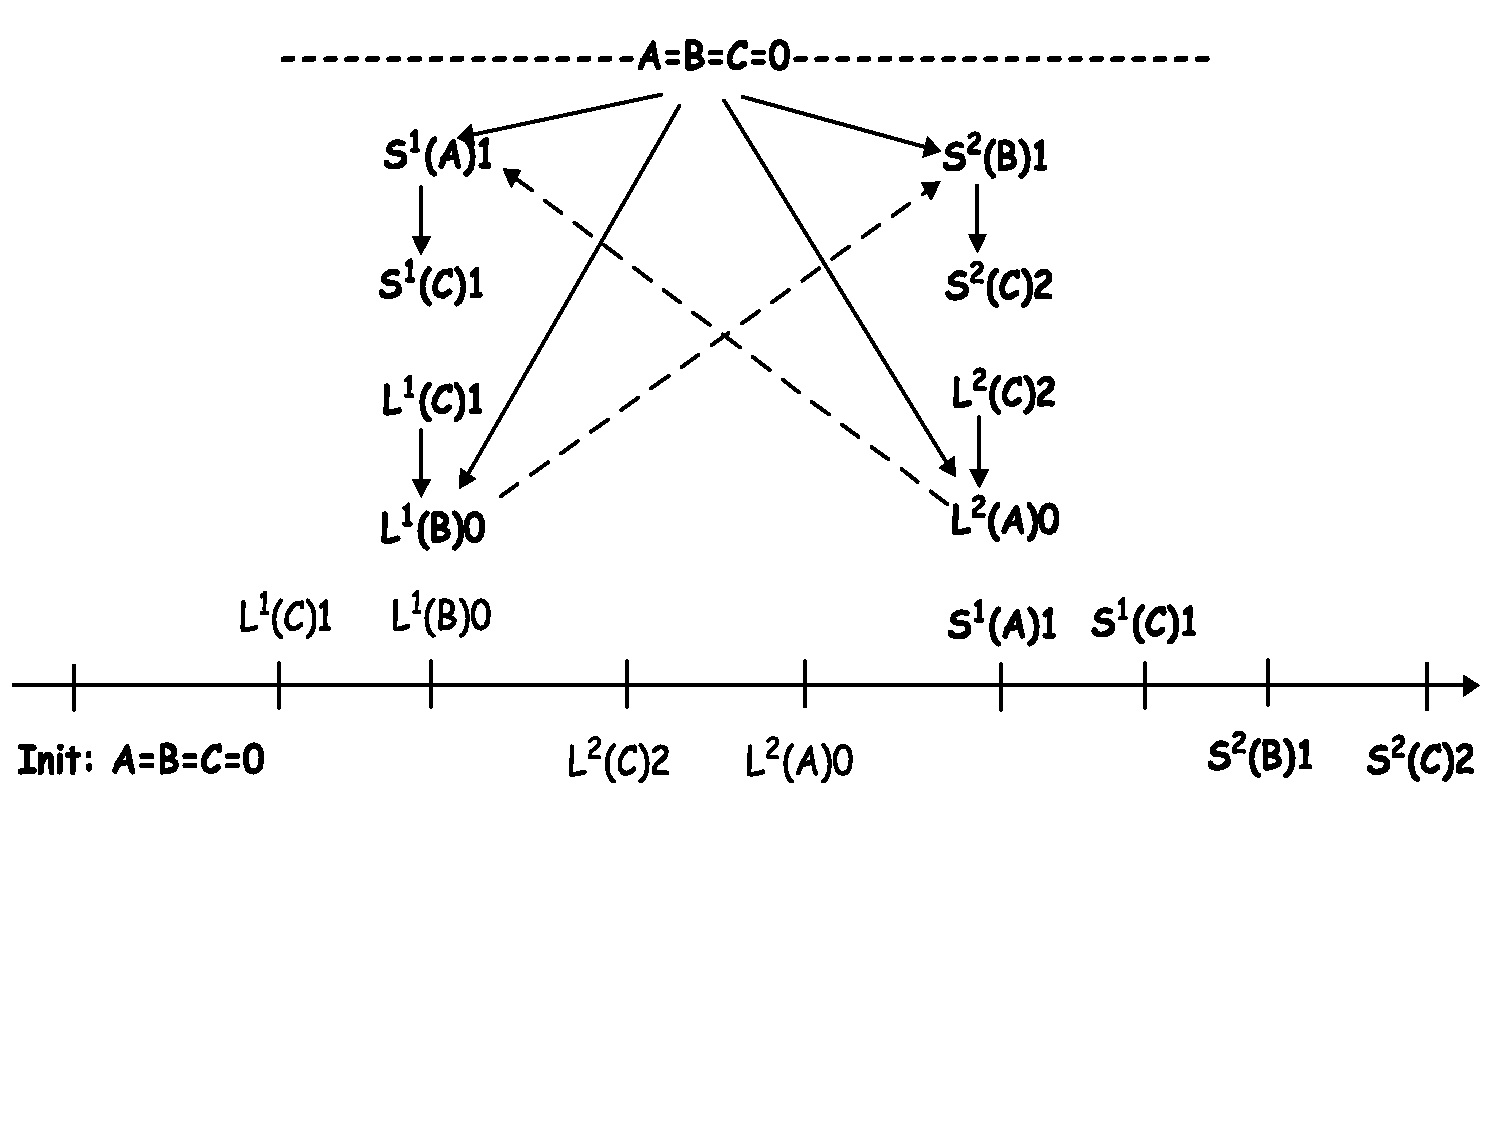
\includegraphics[width=39ex]{Ch7Figs/TSOfwdGraph}\pause
\column{0.55\textwidth}
\vspace{-9ex}
\begin{itemize}
    \item \alert{Remember: Abstract View of Memory Behavior:}
    \item SB is the Private Store Pipeline.
    \item as long as a store can only be observed by its thread $\Rightarrow$
            it does not have to be propagated to others, but
    \item as soon as it can be observed by others it must become visible to all, atomically!
%    \item E.g., private, lockup-free L1 then its thread can use NOT-GPed L1 values,   
%    \item but if L1 shared by several threads, it may not use non-GPed values!
    \item \emp{Graph is for No Forwarding:}
    \item exec: valid but NOT coherent
    \item \emph{With Forwarding $\Rightarrow$ arrow from store to load of {\tt C} $\Rightarrow$ cycles in graph $\Rightarrow$ invalid execution.}
\end{itemize}
\end{columns}
\end{frame}

\begin{frame}[fragile,t]
\frametitle{SUN Micro Relaxed Memory Model (RMO)}

\begin{itemize}
    \item \emp{\bf In RMO only intra-thread dependency order is enforced},
            i.e., there is no implicit order between threads\medskip

    \item \emp{\tt MEMBAR} instructions specifies inter-thread orders explicitly:
    \begin{itemize}
        \item 4 bits used to specify up to 4 orders
        \item \emp{\bf Load-Load}: fence forcing all preceding loads to GPed before any subsequent load may issue,
        \item \emp{\bf Load-Store}: all preceding loads GPed before subsequent store,
        \item \emp{\bf Store-Store}: all preceding stores GPed before subsequent store,
        \item \emp{\bf Store-Load}: all preceding stores GPed before subsequent load.
    \end{itemize}
    \item {\tt MEMBAR} instructions inserted by compiler or programmer.
\end{itemize}
\end{frame}

\begin{frame}[fragile,t]
\frametitle{SUN Micro Relaxed Memory Model (RMO)}

\begin{block}{Use of MEMBAR instructions}
\begin{columns}
\column{0.15\textwidth}
\begin{colorcode}[fontsize=\scriptsize]
            INIT: A := B := 0; 

//T1
A := 1;

\alert{// Non-SC: Valid Exec May Result in (A,B) = (0,1)}


            INIT: A := B := 0; 

//T1
A := 1;


\emph{// SC Execution Cannot Result in (A,B) = (0,1)}
\end{colorcode} 
\column{0.23\textwidth}
\begin{colorcode}[fontsize=\scriptsize]

//T2
while(A==0) ;
B := 1;





//T2
while(A==0) ;
MEMBAR 0100
B := 1;

\end{colorcode} 
\column{0.15\textwidth}
\begin{colorcode}[fontsize=\scriptsize]

//T3
print(B);
print(A);





//T3
print(B);
MEMBAR1000
print(A);

\end{colorcode} 
\column{0.3\textwidth}
\begin{itemize}
    \item first code may yield Non-SC outcome\bigskip
    \item second code may not:
    \item 4 bits specify orders\smallskip
    \item 1000: load-load
    \item 0100: load-store
\end  {itemize}
\end{columns}
\end{block}
\end{frame}


\begin{frame}[fragile,t]
\frametitle{MCM Using Synchronization}

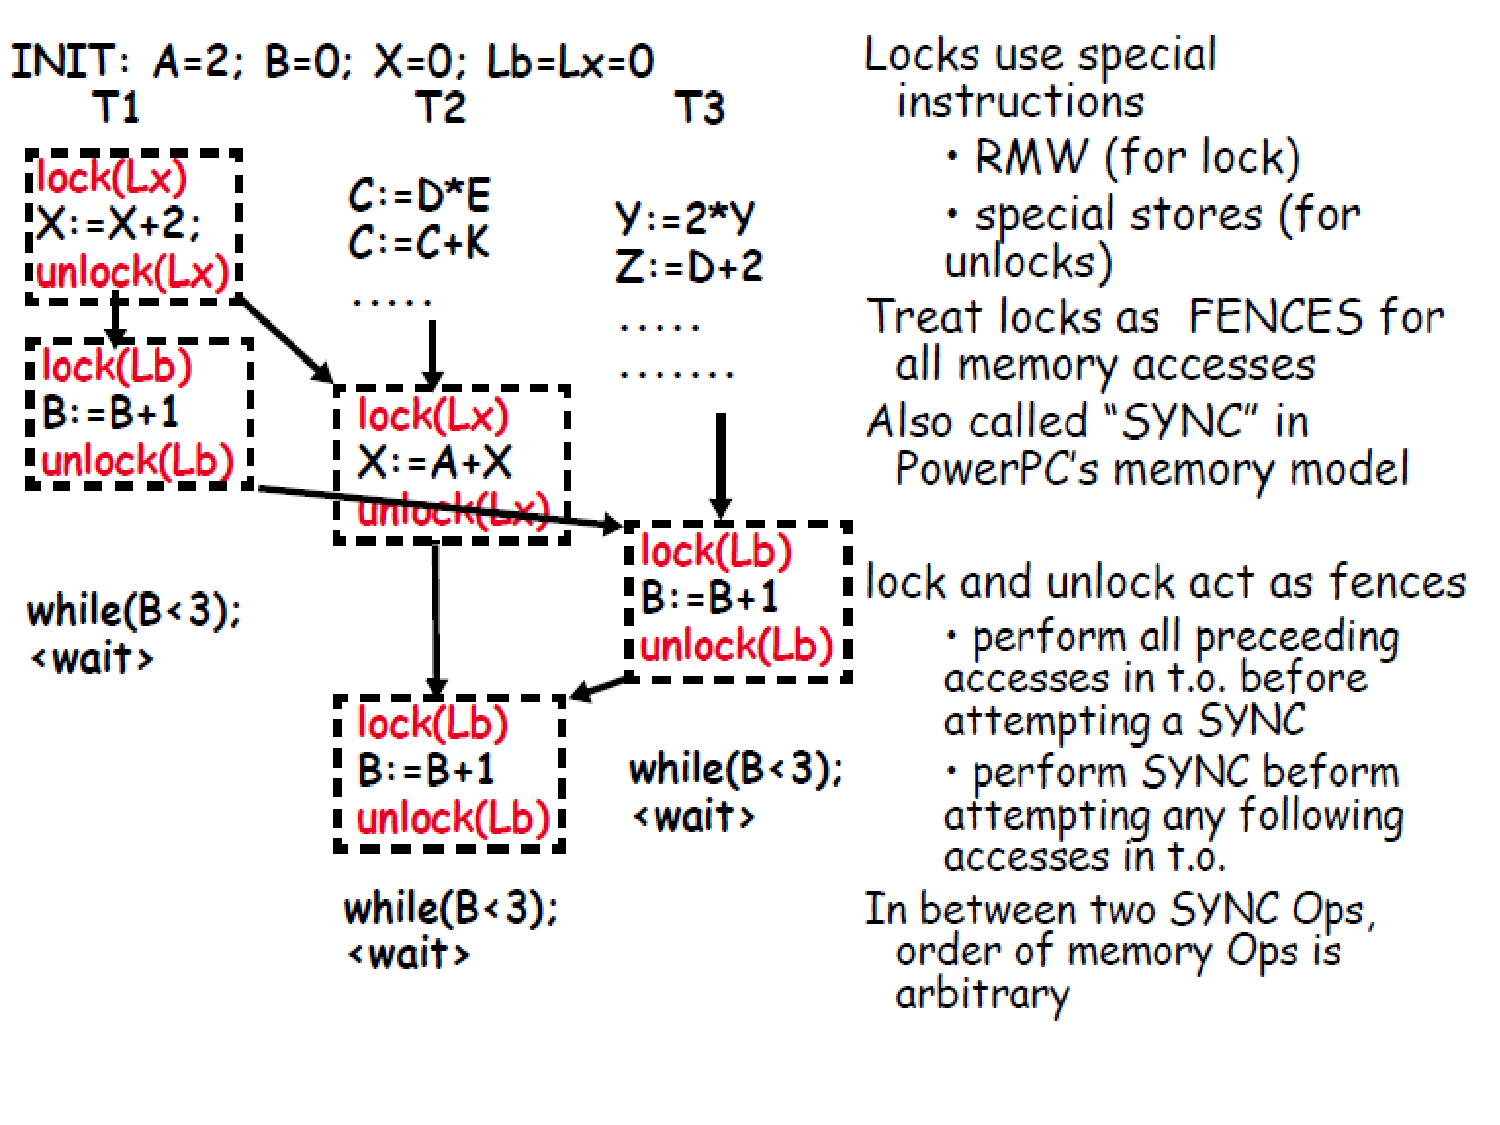
\includegraphics[width=65ex]{Ch7Figs/MCSsync}

\end{frame}


\subsection{Weak Ordering}

\begin{frame}[fragile,t]
\frametitle{Weak Ordering}

\begin{itemize}
    \item Multi-Threaded execution uses locking to avoid race conditions.\medskip

    \item Execution involves several stages
        \begin{itemize}
            \item accesses to private or read-only shared data: unprotected,
            \item accesses to shared modifiable data: protected by locks/barriers.
        \end  {itemize}\medskip

    \item In each phase thread has exclusive access to all its data,
            i.e., no other thread can write or read the data it modifies.\medskip 

    \item \emp{\bf Access to synchronization data}, including all locks in sync protocol,
                treated differently by hwd than ``regular'' accesses:
        \begin{itemize}
            \item They act as fences on all accesses,
            \item Must Globally Perform all accesses preceding SYNC (in TO)
            \item Must Globally Perform SYNC accesses BEFORE all subsequent accesses (in TO)   
        \end  {itemize}\medskip

\end{itemize}

\end{frame}

\begin{frame}[fragile,t]
\frametitle{Weak Ordering}

\begin{itemize}
    \item Access to (Non-SYNC) shared and private data must enforce 
            uniprocessor dependencies (thread order TO) \medskip
        \begin{itemize}
            \item no other requirements, e.g., coherence NOT required,
        \end  {itemize}\medskip

    \item Variables used for synchronization MUST be declared as such,
            so that special instructions can be issued by compiler, 
            e.g., fences.
\end{itemize}

\begin{columns}
\column{0.33\textwidth}
\begin{colorcode}
        INIT: X := FLAG := 0
//P1
X    := 1;
\alert{FLAG} := 1;

        INIT: A := B := 0
//P1
\alert{A} := 1;
while(\alert{B}==1) ;
<critical section>
\alert{A} := 0;
\end{colorcode} 
\column{0.33\textwidth}
\begin{colorcode}

//P2
while(\alert{FLAG} == 0) ;
print(X)


//P2
\alert{B} := 1
while(\alert{A}==1) ;
<critical section>
\alert{B} := 0
\end{colorcode} 
\column{0.3\textwidth}
In the first code {\tt FLAG} must be declared as SYNC variable.\bigskip

In the second code both {\tt A} and {\tt B} must be declared as SYNC variable.
\end{columns}
\end{frame}


\begin{frame}[fragile,t]
\frametitle{Weak Ordering}

\begin{itemize}
    \item Special treatment for read-modify-write {\tt RMW} accesses:  
            it is Globally Performed when both the load \alert{AND} 
            the store are globally performed and atomic.\bigskip
        

    \item SYNC operations must be recognizable by hardware at ISA level, e.g., 
            {\tt T\&S} instruction, and special load and store instructions for
            SYNC variables\bigskip

    \item \emp{\bf Orders to Enforce}, where {\tt Op} denotes regular 
                load/store, and {\tt Sync}  {\tt T\&S,CAS,SWAP}, etc
\end{itemize}

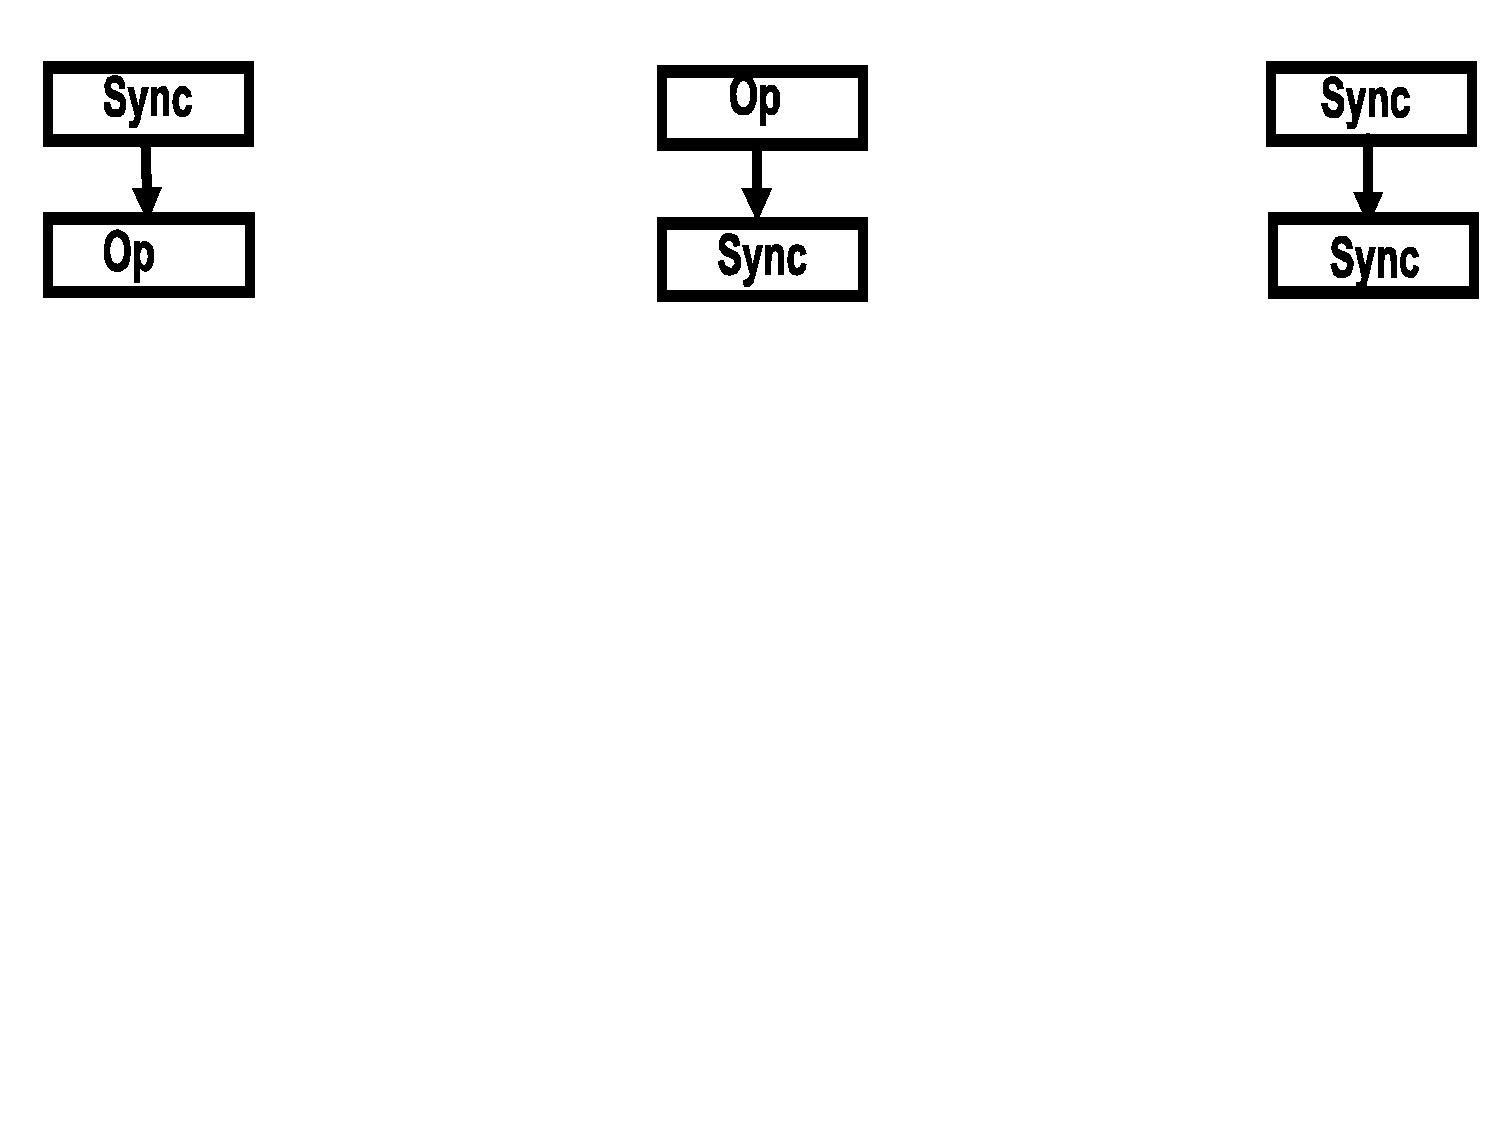
\includegraphics[width=55ex]{Ch7Figs/WeakOrdering}

%\begin{columns}
%\column{0.48\textwidth}
%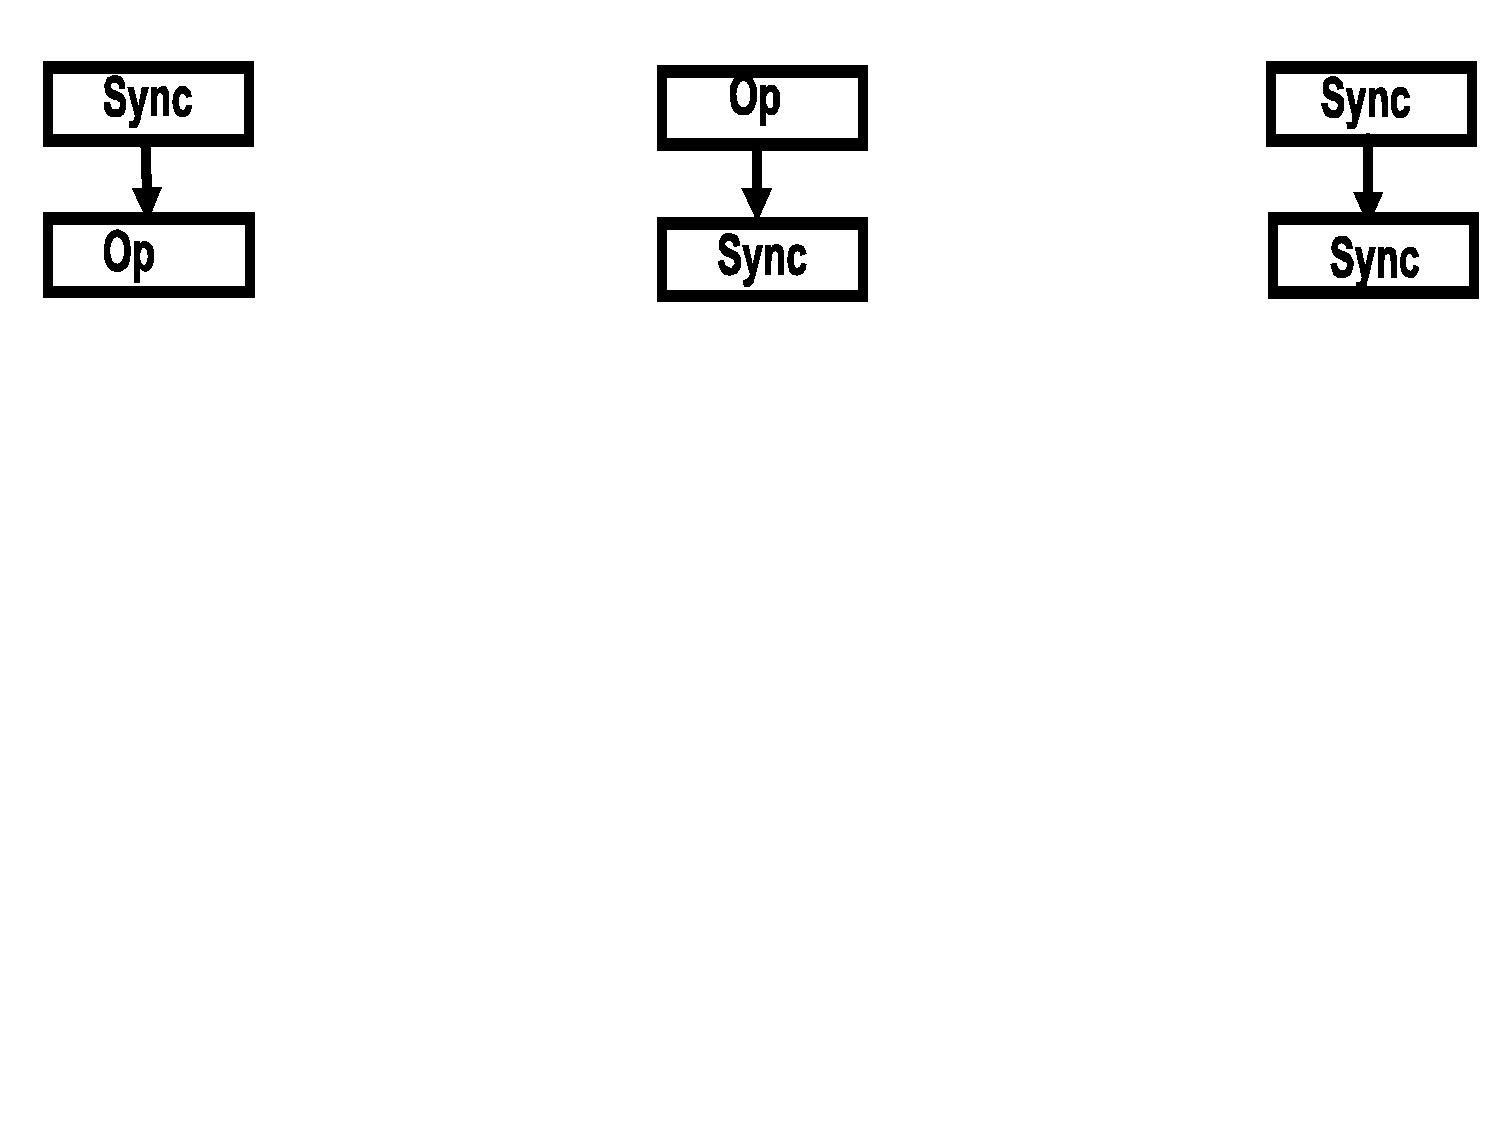
\includegraphics[width=39ex]{Ch7Figs/WeakOrdering}\pause
%\column{0.55\textwidth}
%{\tt OP}: regular load/store
%{\tt SYNC}: $\forall$ synch access, e.g., {\tt T\&S, CAS, SWAP}.
%\end{columns}
\end{frame}


\begin{frame}[fragile,t]
\frametitle{What Does Weak Ordering Mean for IO Procs?}
\vspace{-3ex}
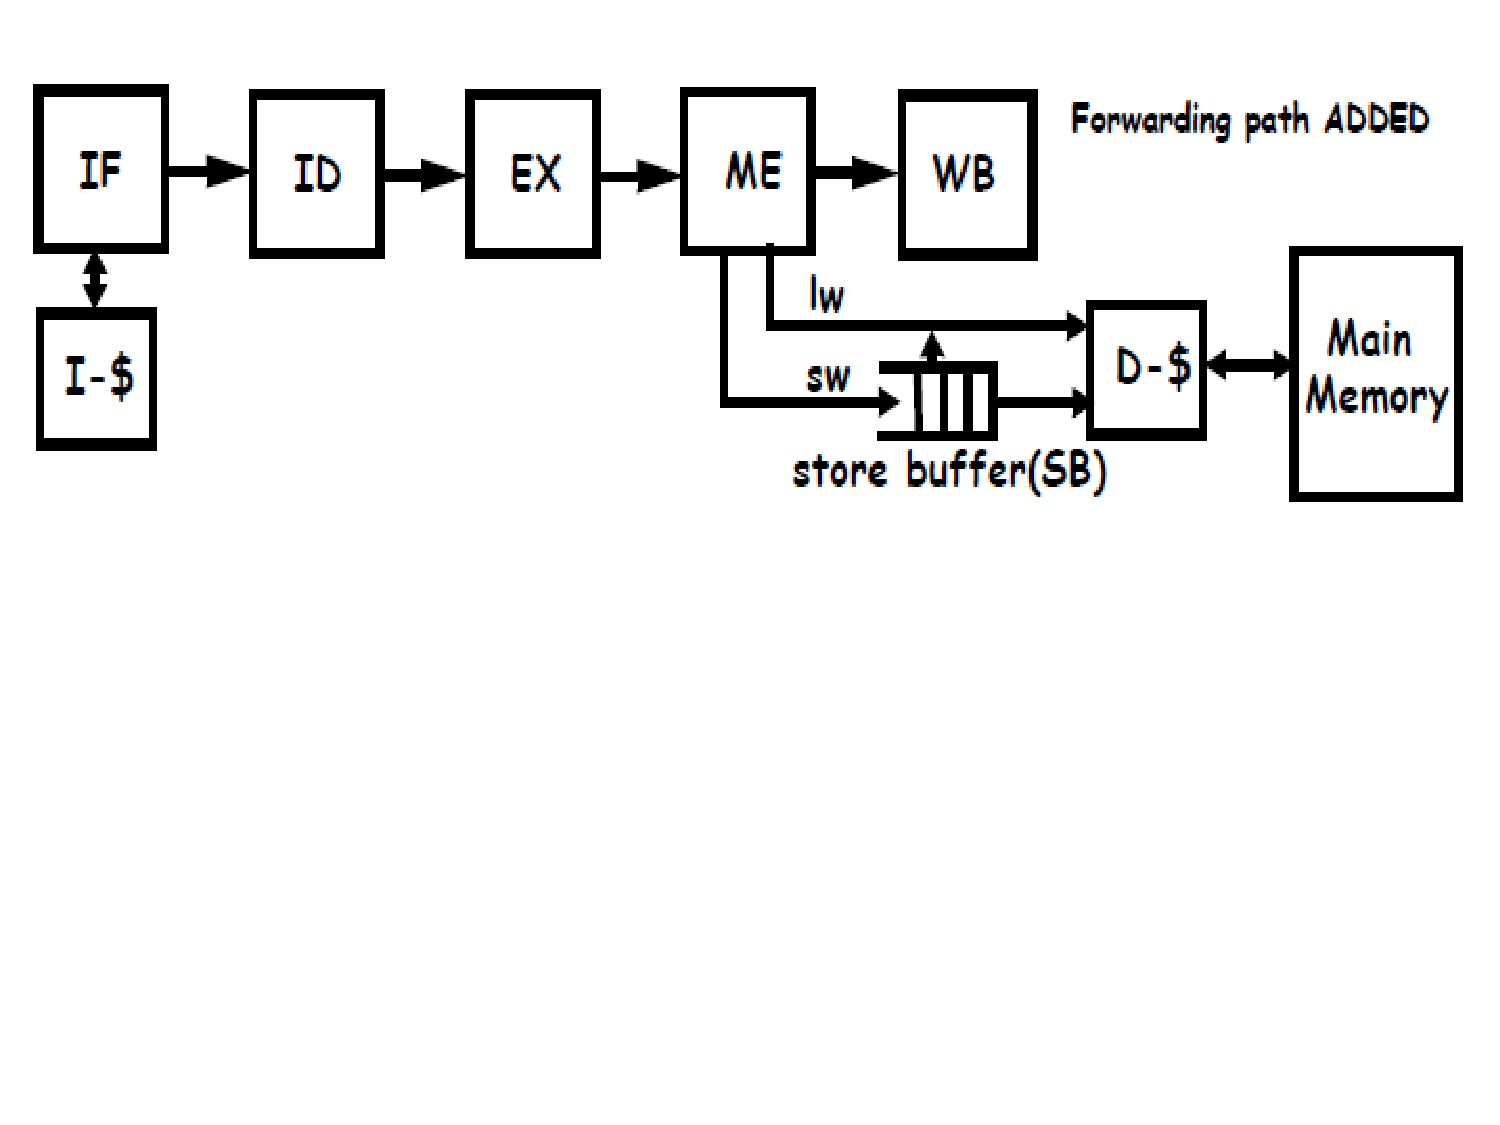
\includegraphics[width=55ex]{Ch7Figs/WeakOrdPipeline}
\vspace{-23ex}

\begin{itemize}
    \item \emph{\bf Loads can return values even if they are not GPed.}\smallskip

    \item \emph{\bf Regular stores in SB executed in any order in parallel.}\smallskip

    \item \emph{\bf Regular Loads never wait for stores and are forwarded.}

    \item \emp{\bf When a {\tt Sync} is executed, it is treated differently:}
        \begin{itemize}
            \item it blocks the entire memory stage until all stores in SB
                    are globally performed. This enforces \emp{\tt Op-TO-Sync}.
            \item \emp{\tt Sync-TO-Op} and \emp{\tt Sync-TO-Sync} 
                    enforced ({\tt Sync} is blocking). % by the IO Processor. 
        \end  {itemize}
\end{itemize}

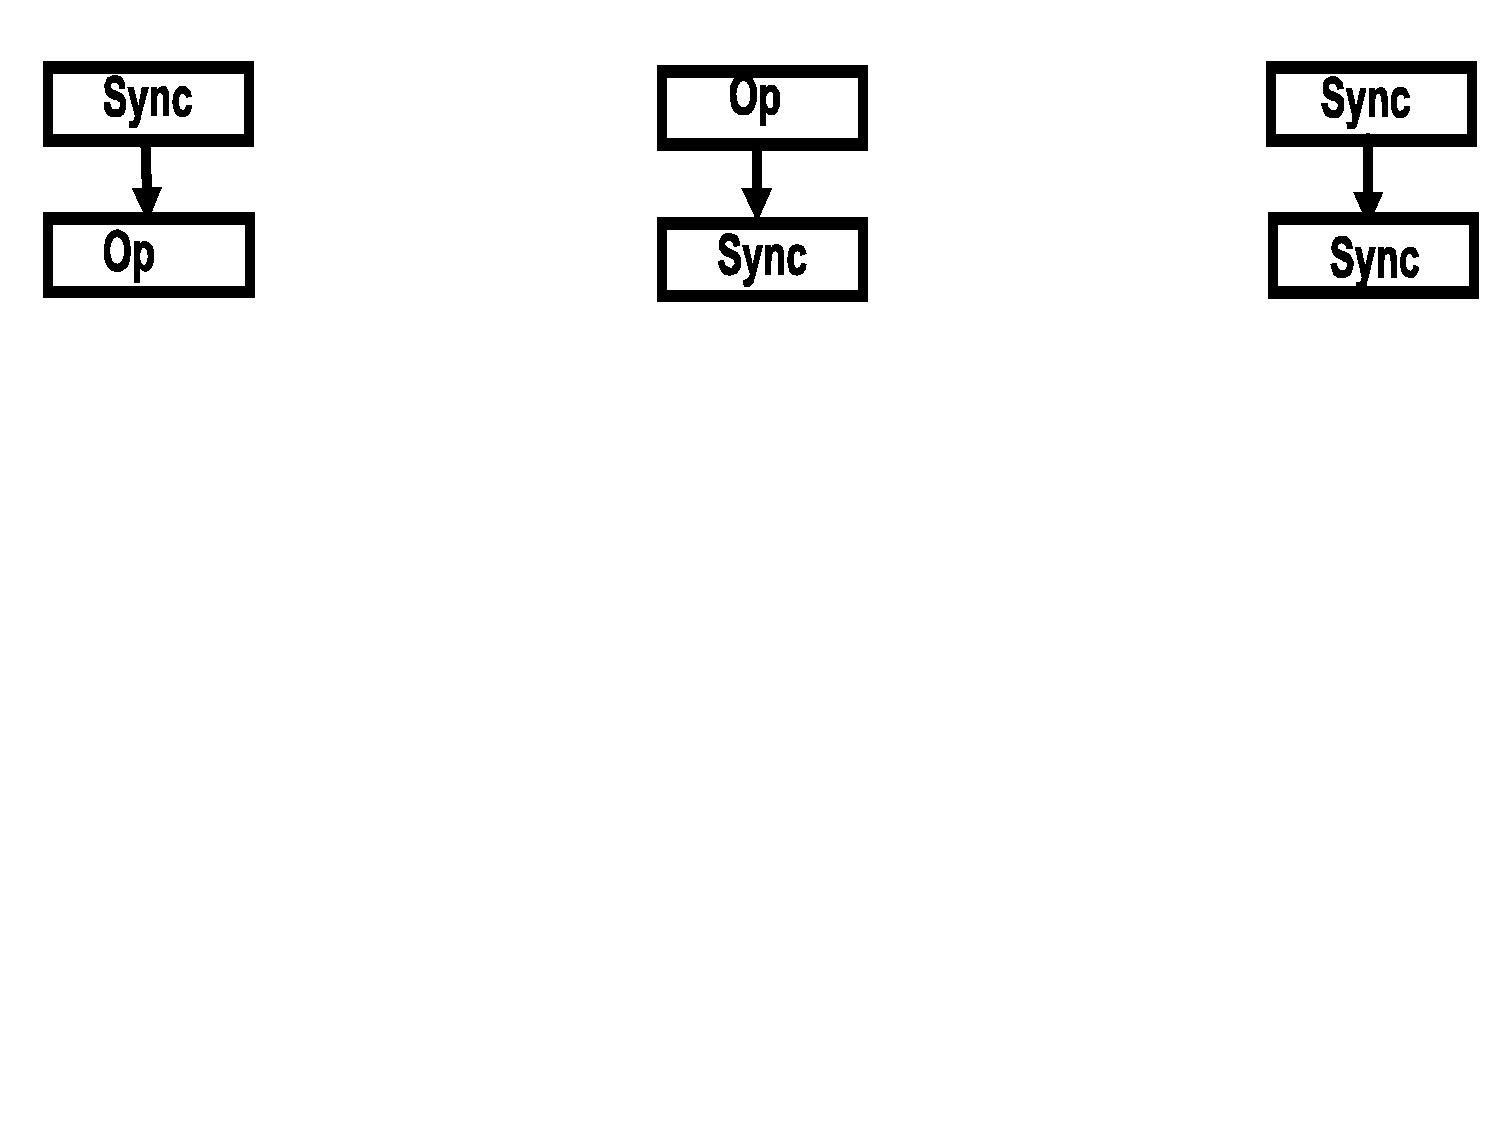
\includegraphics[width=55ex]{Ch7Figs/WeakOrdering}

\end{frame}

\subsection{Release Consistency}

\begin{frame}[fragile,t]
\frametitle{Release Consistency}

\begin{itemize}
    \item Is a More-Relaxed refinement of Weak Ordering:
        \begin{itemize}
            \item distinguish between acquire and release phases:
            \item \emp{Acquire} must be globally performed 
                        before executing subsequent instrs,
            \item all memory operations must be globally performed 
                        BEFORE a \emp{release} can start. 
        \end  {itemize}\medskip

    \item Programmers must declare synchronization as 
            \emp{acquire} and \emp{release} stages\medskip

    \item \emp{Acquires and Releases} \emph{\bf Must Be Sequential Consistent. Orders to Enforce:}
\end{itemize}

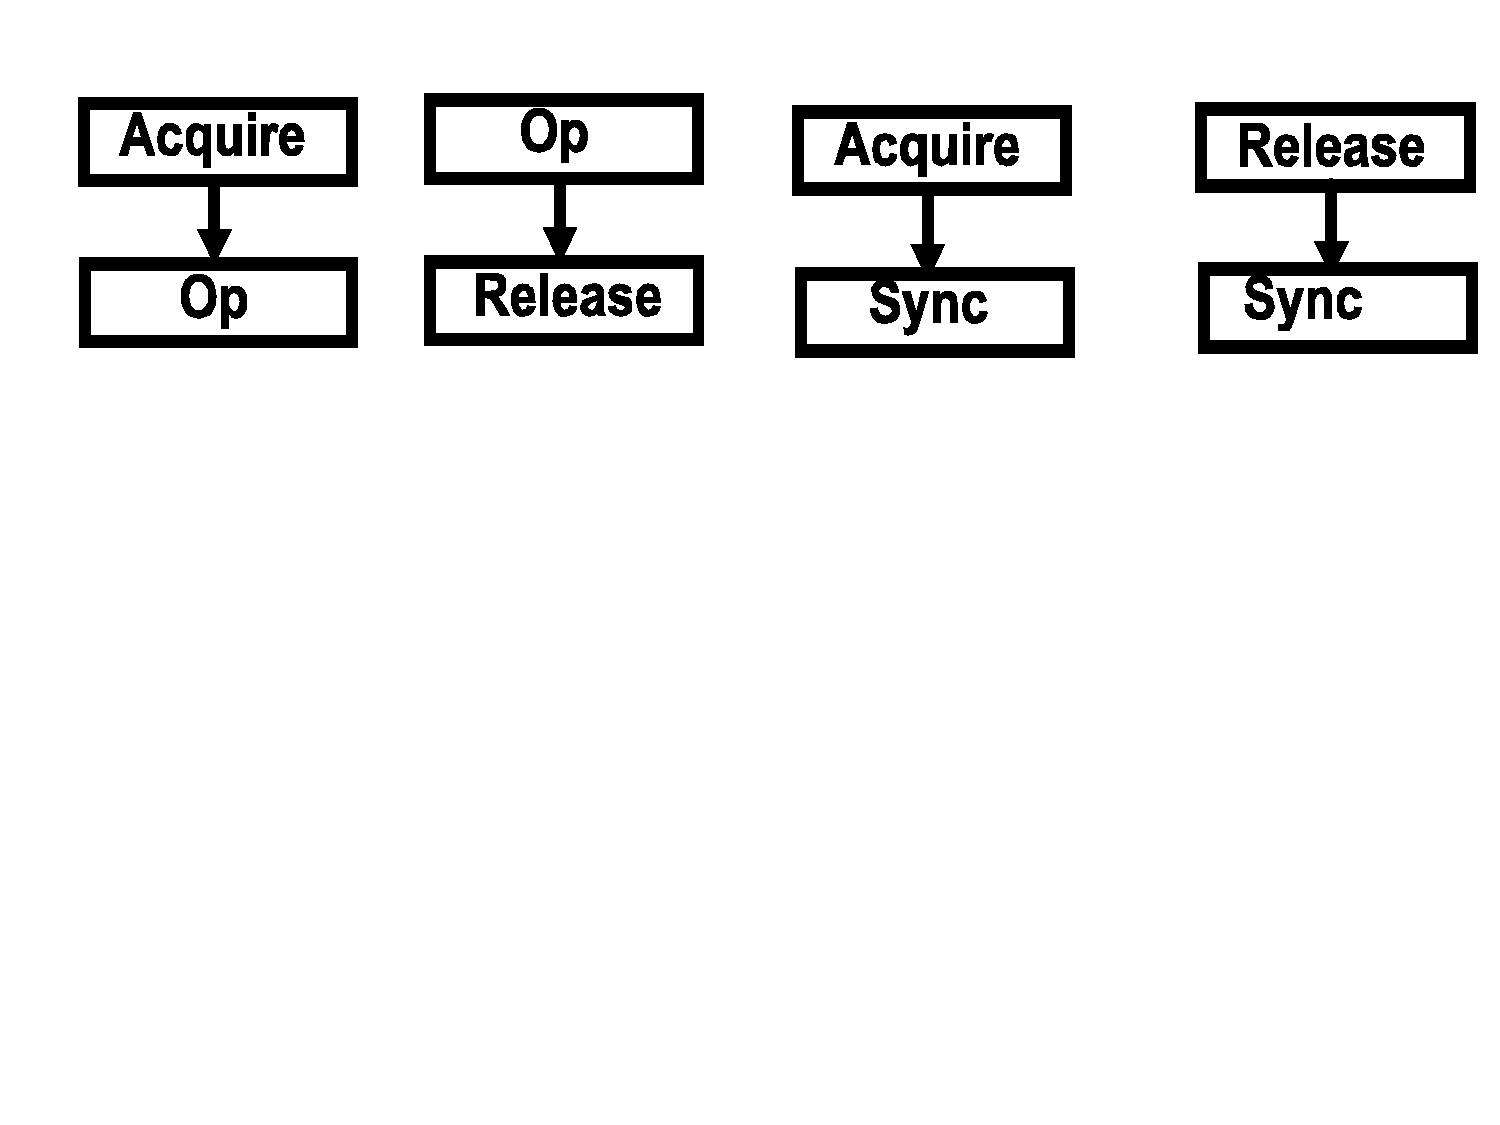
\includegraphics[width=55ex]{Ch7Figs/ReleasedOrdering}

\end{frame}

\begin{frame}[fragile,t]
\frametitle{Release Consistency Example}
\vspace{-3ex}
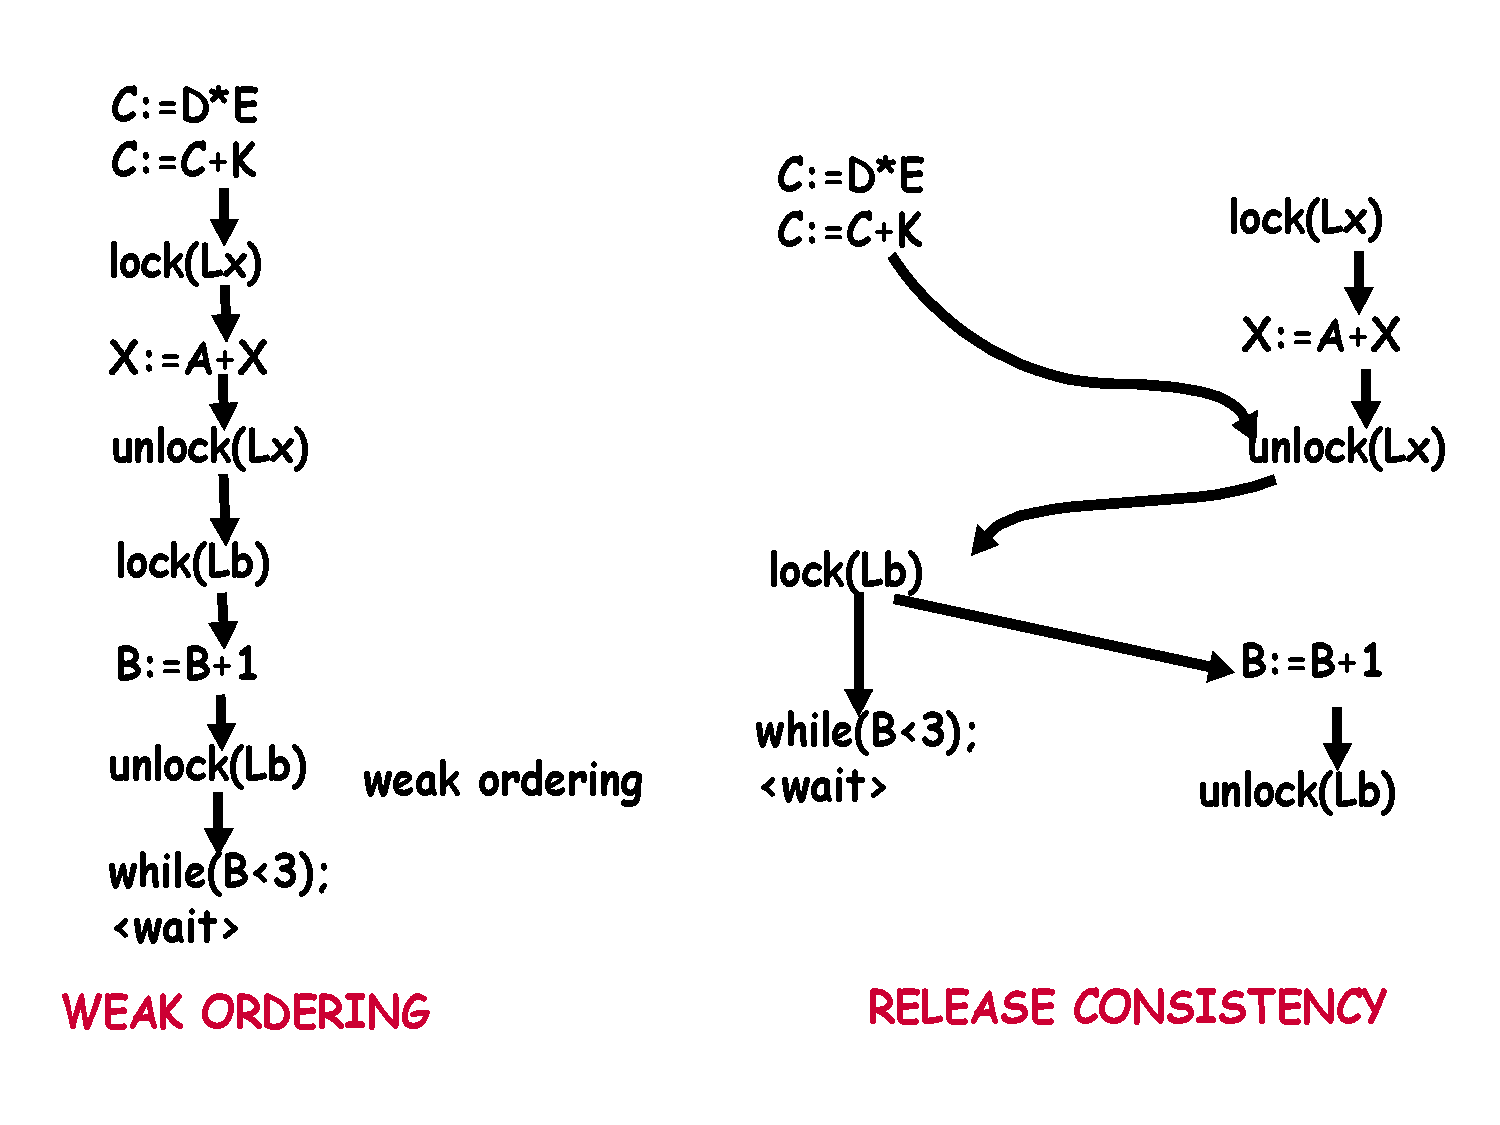
\includegraphics[width=55ex]{Ch7Figs/ReleasedConsistGraph}
\vspace{-4ex}

\begin{itemize}
    \item Significantly more ILP in Release Consistency:
        \begin{itemize}
            \item code before {\tt Unlock(Lx)} can be executed in parallel.
            \item code after {\tt Lock(Lb)} can all be executed in parallel. 
        \end  {itemize}\medskip

    \item Challenge is to take advantage of it within each thread!
\end{itemize}
\end{frame}


\begin{frame}[fragile,t]
\frametitle{What Does Release Consistency Mean for IO Proc?}
\vspace{-3ex}
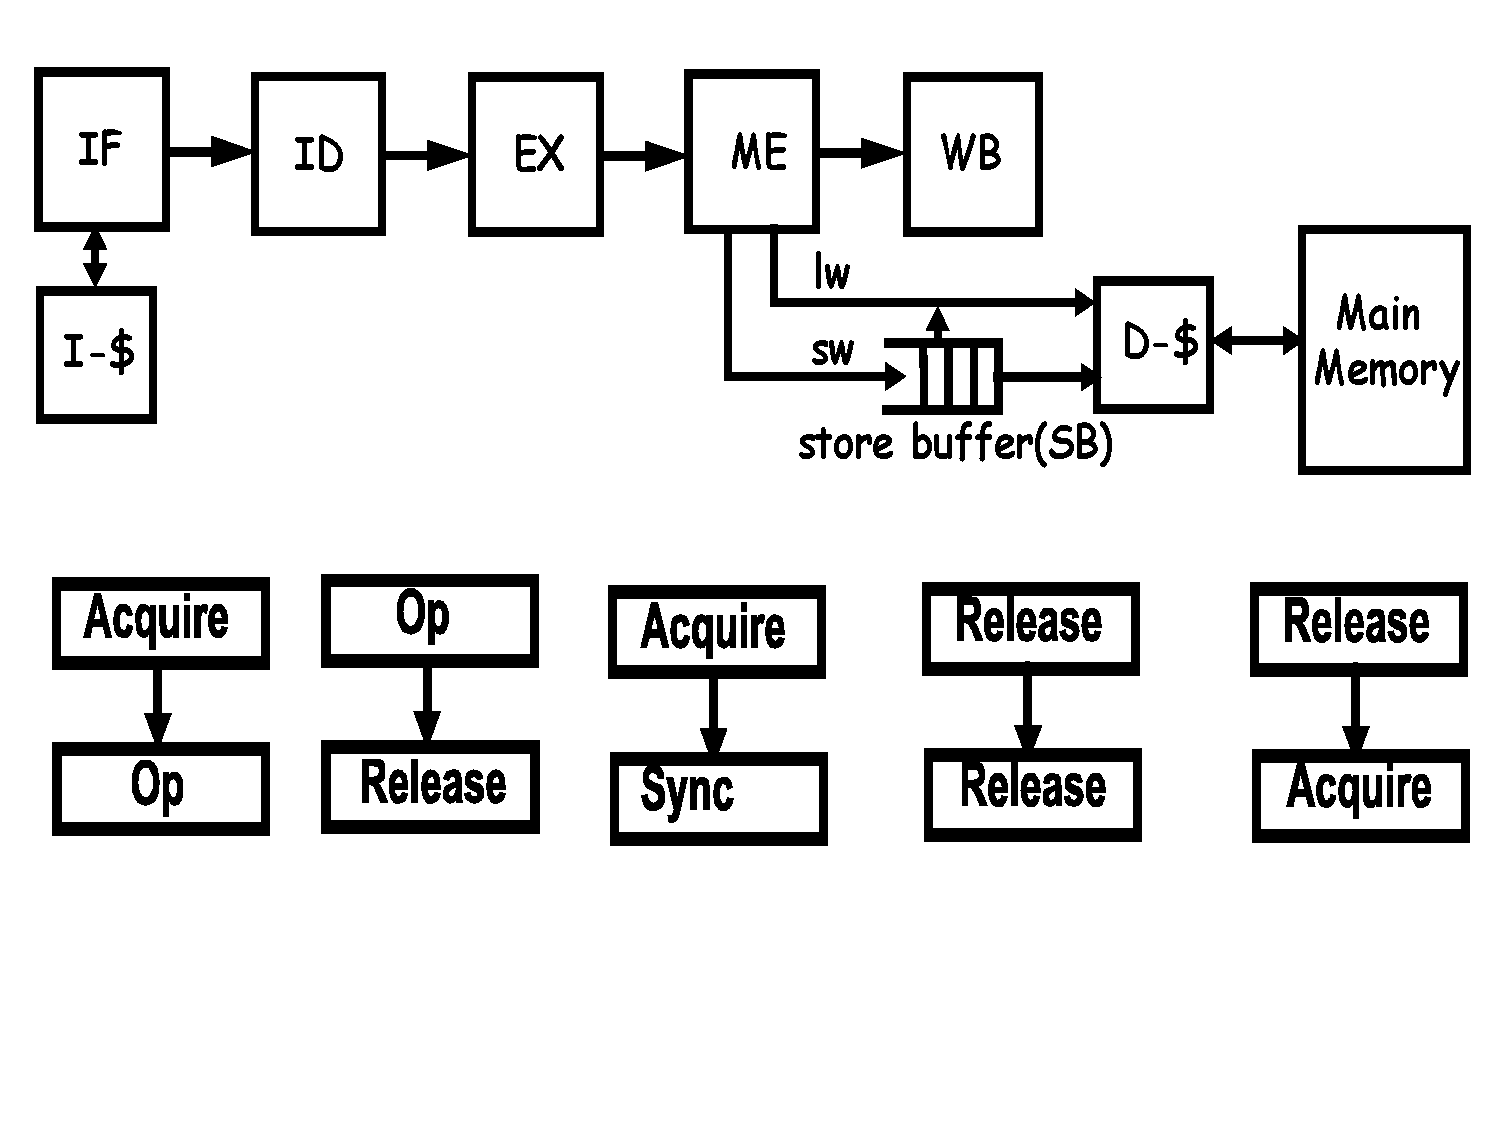
\includegraphics[width=44ex]{Ch7Figs/ReleasedIOpipeOrd}
\vspace{-8ex}

\begin{itemize}
    \item \emph{\bf No Ordering for Regular Load/Stores} (return non-GPed vals)\smallskip
        \begin{itemize}
            \item regular stores in SB can be executed in any order in parallel,
            \item regular loads are forwarded \& never wait for regular stores in SB.
        \end  {itemize}

    \item \emph{\bf Acquires are blocking $\Rightarrow$} 
                \emp{\tt Acquire-Op/Sync} \emph{\bf auto enforced}\smallskip

    \item \emph{\bf A Release is inserted in SB with regular loads}
        \begin{itemize}
            \item Releases must wait in SB until all prior stores and releases are GPed
                    $\Rightarrow$ \emp{\tt OP-Release} and \emp{\tt Release-Release} enforced 
                %(because previous loads have already retired),
            \item Acquire waits until all prior releases in SB 
                    have been GPed $\Rightarrow$ \emp{\tt Release-Acquire} enforced.
        \end  {itemize}
\end{itemize}

\end{frame}

\end{document}
